\documentclass[a4paper]{article}
% \usepackage{fullpage}
% \usepackage[top=1.5cm, bottom=1.5cm, left=2cm, right=2cm]{geometry}
\usepackage{amsmath}
\usepackage{graphicx}
\usepackage{geometry}
% \usepackage{floatrow}
\usepackage{layout}
\usepackage{amssymb} 
\usepackage{multirow}
\usepackage{caption}
\usepackage{pgfgantt}
\usepackage{float}
\usepackage{hyperref}
\usepackage{glossaries}
\usepackage{listings}
\usepackage{hyperref}
\usepackage{amsmath}
% \usepackage{caption}
% \usepackage{subfigure}
\usepackage{tikz}

\usepackage{titlesec}

\setcounter{secnumdepth}{4}

\titleformat{\paragraph}
{\normalfont\normalsize\bfseries}{\theparagraph}{1em}{}
\titlespacing*{\paragraph}
{0pt}{3.25ex plus 1ex minus .2ex}{1.5ex plus .2ex}



\usetikzlibrary{calc,intersections,through,backgrounds,angles,quotes}


\geometry{margin=1.0in}
\usepackage{authblk}
\usepackage{indentfirst}
 

\begin{document}
\pagenumbering{roman}

%----------------------INITIALIZE TABLE PARAMETERS------------------------%
\newcommand\mTitle{\textbf{}}
\newcommand\mNumber{}
\newcommand\mLocation{}
\newcommand\mDate{}
\newcommand\mDuration{}
\newcommand\mAttendies{}
\newcommand\mMinuteTaker{}
\newcommand\mDiscussion{}
\newcommand\mFuturePlans{}
\newcommand\mDeadlines{}
%%%%%%%%%%%%%%%%%%%%%%%%%%%%%%%%%%%%%%%%%%%%%%%%%%%%%%%%%%%%%%%%%%%%%%%%%%

\title{TME-180 Final report\\ 
\textbf{Variables extraction and trajectory reconstruction for
modelling driver behaviour}}
\author{\textbf\large{Ahmed Hamdy Shams El Din}\\
        \textbf\large{Mohamed Takkoush}\\
        \textbf\large{Nicklas Pettersson}\\
        \textbf\large{Sriranga Hulkunte Gopinath}}
%\affiliation{The	College,	University	of	Chicago,	Chicago,	Illinois	60637,	USA}
\affil{\textbf{Chalmers University of Technology, Gothenburg, Sweden}}
\date{\today}
%	Abstract
\maketitle
\begin{abstract}
Active safety and autonomous driving are two booming words in the automotive industry of today. Most, if not all, companies are in a race to provide a safe environment for driving and are thriving to reach their goals in producing autonomous vehicles. 

The general goal of this project is to develop a human driver model for critical lane-changing manoeuvres. Annotation of such data was done manually on videos acquired from dash-cam footage from a naturalistic driving study (NDS) by identifying different events in time, such as time of lane crossing and relative distance between vehicles. A semi-automatic tool to aid the annotation of the NDS footage was developed and several methods for range calculation are discussed such as the pixel width method and the triangulation method, which are also used for calculating the heading angle and the lateral offset of the lead vehicle. The results were found to be relatively accurate considering the simplicity of the tool.  As for the tracking of the lead vehicles and the lanes, the most accurate method was found to be through interpolating between user inputs.
\end{abstract}%\maketitle
\newpage
\section*{Acknowledgement}

\noindent
This work has been performed under the VTTI Data License Agreement. The findings and conclusions of this report are those of the authors and do not necessarily represent the views of VTTI, the Transportation Research Board, or the National Academies.
\noindent

\noindent
\\
Special thanks to the project supervisors \textbf{Jonas Bärgman} and \textbf{Giulio Bianchi Piccinini} for their support during the course of this project. Their guidance and understanding helped us during tough weeks, and their encouraging recommendations were paramount for writing the report. We would also like to thank our families and friends who stood by our side with mental support since the day we started on the project up until this moment.


% \textcolor{red}{You need to have an Acknowledgement section with, at least, the following information: "The findings and conclusions of this report are those of the authors and do not necessarily represent the views of VTTI, the Transportation Research Board, or the National Academies" You will also need to include the following statement included: "This work has been performed under the VTTI Data License Agreement (DUL): SHRP2-DUL-16-204.}

\newpage
\tableofcontents
\newpage
\pagenumbering{arabic}
%%	Main	body	starts	here

\section*{Abbreviations}
\addcontentsline{toc}{section}{Abbreviations}
\begin{itemize}
    \item NDS - Naturalistic driving study
    \item NDD - Naturalistic driving data
    \item VTTI - Virginia Tech Transportation Institute
    \item SV - Subject vehicle
    \item POV - Principle object vehicle
    \item GUI - Graphical user interface
    \item VP - Vanishing point
    \item ROI - Region Of Interest
\end{itemize}



\newpage

\section{Introduction}
\label{sec:Intro}
%	Introduction
Understanding human behaviour is an important step for the development of computational driver models. These models are currently used in the evaluation of modern active  systems \cite{bargman2017counterfactual}. Through the analysis of  videos collected during naturalistic driving studies, information about driving behaviour can be obtained and used for the development of driver models. However, the retrieval of information from Naturalistic Driving Studies (NDS) often requires manual annotations of the data, which is a time consuming task \cite{DOZZA2013298}.

This project aims to develop a tool that can support the manual annotations of NDS, with the final objective to increase the accuracy of the annotations and reduce the time required to extract the variables. The safety-critical target scenario under evaluation for the development of the tool is the lane change manoeuvre: in this safety-critical target scenario, the lead vehicle  attempts or succeeds to change lane in front of the following vehicle, causing the driver of the following vehicle to perform an evasive manoeuvre (brake or steer away) to avoid a crash. In this report, the lead vehicle will be referred to as the Principal Object Vehicle (POV) and the following vehicle referred to as the Subject Vehicle (SV). 

The developed tool utilizes a video of the forward roadway recorded by the camera installed in the SV. The expected outputs from the tools are variables, such as the speed of the POV, the distance between the SV and the POV, the distance between the POV and the lane marks. The extracted variables can be used to develop driver models describing the SV drivers' response to the lane change of the POV.

% If possible, the tool will finally be evaluated using data collected from a small scale experiment with a vehicle equipped with reference measurement systems (e.g forward video camera) close to the one used in the specified data-set.

The stakeholders of this project are AB Volvo and Zenuity, who occasionally took part in meetings and attended the presentations. The suggestions and needs of the stakeholders were considered while developing a dynamic tool for different uses.



\subsection{Background}

The field of traffic safety has seen huge developments since the introduction of the automobile. Initially, passive safety systems were introduced to prevent or reduce injuries in case of a crash \cite{bishop2005intelligent}. These systems - such as crumble zones, seat belts and airbags - are built in the vehicle structure and are designed to restrain the occupant and absorb energy in case of a crash. As technology and the increased use of electronics in vehicles progressed, engineers have been able to develop active safety systems that are designed to prevent a crash from happening, for example, Electronic Stability Program (ESP), Lane Departure Warning (LDW) and Automatic Emergency Braking (AEB). Active safety systems could either issue warnings to the driver, such as LDW, or make corrections to help the driver avoid a crash, such as ESP \cite{bishop2005intelligent}.  

Driver models serve as an important input in developing active safety systems: driver models can for example be used for the assessment of predictive safety benefits and for the definition of warning strategies. Driver models are used to predict human behaviour in different critical scenarios, and act upon these predictions to mitigate or reduce the severity of crashes \cite{bargman2017counterfactual}. There are different driver models with different complexities. 

One well known model is the 
car-following model presented by Gazis, Herman, and
Rothery (1961). In this model, the diver aims to keep the same speed as the  lead vehicle and adapts to speed changes faster at higher speed, low headway distances . Parameters for this model were tuned through conducting follow-the-leader experiments \cite{bexelius1968extended}. This model was later extended to account for a number of error-inducing driver behaviours and stochasticity and have been used for evaluating active safety systems, such as FCW \cite{markkula2012review}. Another way to gather data about driver behaviour for these models is through NDS.
% These models will also become important for the development of autonomous vehicles, that will most likely drive on roads among normal vehicles driven by humans. It is then crucial that an autonomous system can predict what surrounding vehicles are going to do and act accordingly. These developments should insure safer roads and better traffic safety. 

NDS is a methodology in which the participants are asked to drive as they would do in their daily life \cite{Udrive} and data are collected from vehicles equipped  with sensors and cameras. The sensors provide variables, such as speed and GPS location, while the two cameras, one pointed at the driver and the other one at the road ahead, provide videos showing the behaviour of the driver and the other road users. 

The data used in this project was collected through the second Strategic Highway Research Program (SHRP2) though a naturalistic driving study involving more than 3000 male and female volunteers, with the aim to learn how individual driver behaviour interacts with vehicle and roadway characteristics \cite{hallmark2011evaluation}. 


\subsection{Aim and Scope}
% The aim is a brief description of the assignment and its intended outcome.

As previously mentioned, the annotation of NDS videos is mostly done manually. Through developing tools to aid this process, a larger set of videos could be annotated in a shorter time, providing more variables to be used for the analysis and modelling of driver behaviour.

Throughout the course of the project, the team aims to develop a semi-automatic tool that aids the annotation of NDS, in lane-change manoeuvres involving two vehicles. The tool will be used to determine variables, such as the distance between the SV and the POV, the POV speed, the distance between the POV and the lane markings, and the positioning of the SV in the lane. The tool should be semi-automatic, meaning that the user will manually annotate features such as the lane markings and the POV width. For this reason, the tool includes a Graphical User Interface (GUI), which could support the performance of manual annotations. 

By using this tool, the accuracy of the estimated variables (e.g. speed of POV and distance between SV and POV) will increase and the time required for the annotations will decrease. As a consequence, the accuracy of the analyses to design driver models developed using NDS will improve.
\subsection{Literature Review}
In order to carry out the study and develop the tool needed for studying drivers' behaviour, a non-exhaustive literature and resource study was carried out regarding state of the art and current resources available to the team.

% \subsubsection{Driver Models}
% Driver models serve as an important input in predicting driver reaction and developing active safety systems. Computational driver models define specific decisions based on previous information in order to carry out a task. Those decisions are translated into computations that the driver system follows \cite{CompDrivMod}. Such models can, for example, be used for the assessment of predictive safety benefits and for the definition of warning strategies. These are used to predict human behaviour in different critical scenarios, and act upon these predictions to mitigate or reduce the severity of crashes.

% There are different driver models with different complexities. One well known model is the 
% car following model presented by Gazis, Herman, and
% Rothery (1961). In this model the diver aims to keep the same speed as the  lead vehicle, and corrects to speed changes faster at higher speed, low headway distances . Parameters for this model were tuned through conducting follow the lead experiments \cite{bexelius1968extended}. This model was later extended to account for a number of error inducing driver behaviours and stochasticity and have been used for evaluating active safety systems, such as FCW \cite{markkula2012review}.




\subsubsection{Camera model and rectification}
To be able to carry out image processing techniques on images, one would first have to determine a camera model and rectify the images in hand for distortions and camera pose. As seen over the years, the pinhole camera model is the most generic camera model used. The theory behind the pinhole camera model is described in details in \cite{xu2013epipolar}. This popular camera model has proven to be a reliable model in several applications such as in close-range \cite{duane1971close} or wide-angle lenses \cite{swaminathan2000nonmetric}. Figure \ref{fig:pinhole_model} shows a basic simplified  pinhole camera model.

\begin{figure}[H]
    \centering
    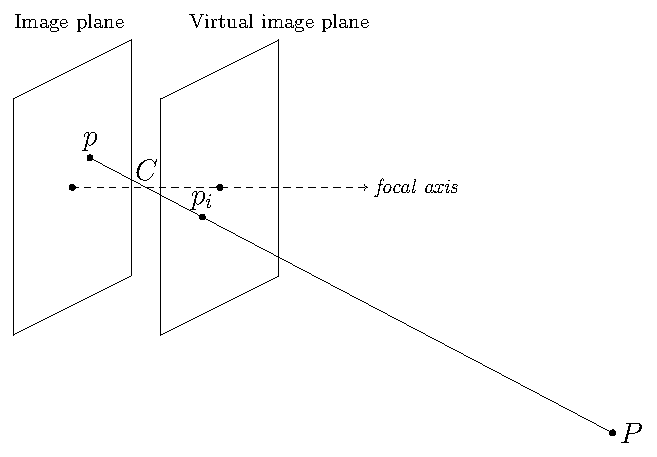
\includegraphics[width = 0.6\textwidth]{Figures/camera_model_1.pdf}
    \caption{Pinhole Camera Model}
    \label{fig:pinhole_model}
\end{figure}

Camera calibration and image rectification are well studied subjects and are becoming  more important with the increasing need for higher accuracy measurement in computer vision. For geometrical measurements, the main concern is camera distortion \cite{wang2008new}.

Radial distortion causes an inward or outward displacement of a given image point from its ideal location while tangential distortion causes a rotational displacement about the center of the image. These effects are better explained with figures in \cite{wang2008new}. These distortions are caused by either the spherical shape or the position of the camera lens and results in straight objects in reality to appear curved in the image. Image rectification is therefore needed to get a better estimation of the real world position of objects in an image.

There are two sets of parameters that are needed for image rectification, these are internal (intrinsic) and external (extrinsic)  camera parameters. Internal parameters determine the image coordinates of a point given the spatial position of said point with respect to the camera. External parameters characterise the geometrical relation between the camera and the scene \cite{wang2008new}. While intrinsic calibration is only done once for a camera, extrinsic calibration is required when the position and orientation of the camera is subjected to large changes, such as the case of a vehicle driving on the road \cite{wang2004simple}. Given a sufficient number of visible points, their placement in the image, and their placement in real world coordinates, the internal and external camera parameters can be estimated \cite{wang2008new}.




\subsubsection{Lane detection}

Lane detection is a crucial part of the development of autonomous vehicles and many active safety systems, such as Lane Keep Assist (LKA), Lane Departure Warning (LDW) and Lane Change Support (LCS). In these applications, lanes are in most cases detected in real-time with computer vision technologies, by using one or multiply road facing cameras mounted at the front of a vehicle. Lane detection is also used to analyse NDS videos in order to extract information about the events that lead to a crash or a near-crash \cite{IEEE2014}. In fact, lane change events, lane type and vehicle localisation using lanes are some of the most important measures when it comes to investigation of crash and pre-crash events \cite{IEEE2014}. The goal of this literature review is to investigate how a lane detection algorithm can be structured and how it can be used in practice.

\paragraph{Algorithm}
A simple but robust lane detection algorithm is described in \cite{Compvision}. The input data to the algorithm is an image captured by a road-facing camera mounted on a moving vehicle. In order to detect the lanes, the image needs to be processed. The basic idea behind lane detection is to identify the lane boundaries, or the edges of the lanes. The edges of the lane can be defined as a rapid change in intensity from one pixel to another. In the case of detecting the lanes on a road, the difference in intensity between the yellow or white lane and the gray asphalt needs to be identified \cite{EdgeDet}. In order to easier detect change in colour, the image in the algorithm \cite{Compvision} is converted to grayscale. An alternative approach is to filter out all the colours in the image except for yellow and white and therefore distinguish the lanes from other objects in the image. The problem with this approach is that worn out lanes have a different colour than newer lanes, and the brightness of the image affects the colour,  making it hard to find a colour threshold which will work in all videos \cite{ColorScale}. The next step in the construction process of the algorithm described in \cite{Compvision} is to remove noise from the image, for example strong shadows. One of the most used filters in these kinds of tasks is the Gaussian blur filters, which is a low pass filter that smoothens the image \cite{GaussianFilter}. There are also filters that adjust the brightness and contrast of the image. The contrast between the asphalt and the lane is identified by using an edge detector.

For the algorithm described in \cite{Compvision}, a canny edge detector was used. In order to determine which of the identified edges are lanes, the algorithm \cite{Compvision} used a Hough transform to search for lines which are horizontal with a maximum of 45 degrees slope to either the left or the right. These identified lines are considered lanes, all the other detected lines are rejected. The last step in the development process of the algorithm described in \cite{Compvision} is to define the region of interest (ROI).  In this step, the processed image is cropped so all unnecessary information in the image is rejected, for example the environment on the side of the road. In this case, ROI only consist of the road near the vehicle.

\paragraph{Critical aspects} 
Even though lane detection methods have been improved during recent years, there are still challenges to overcome in this field. Complex illuminations and shadows from the environment can cause the camera to miss lanes on the road, or wrongly recognise objects and shadows as lanes \cite{Compvision}. The ability of the algorithms to detect lanes is heavily dependent on the time of the day, the weather and the season of the year. In order for the lane detection algorithm to be robust, it must be able to detect the lanes in different conditions.

\subsubsection{Heading angle and lateral offset estimation}
Calculating the heading angle of the POV is not an easy task, especially using a mono camera system. 

In \cite{3dtrajectory}, the authors estimate the 3D pose of an object by following some feature points between frames and constructing a 3D trajectory as well as the object's structure. The estimation is fortified by using the optical flow of the feature points. A more straightforward method is introduced in \cite{realtimePoseEstimation} where an extended Kalman filter is used to estimate the rotation and translation of an object between frames, given that the feature points' coordinates are known in 3D-space and 2D-space.

Another method, proposed in \cite{FeatureBasedHomography}, utilises the concept of homography for calculating the change in a plane between frames. This method was intended to calculate the angular rate of a POV along intersections and curves. The calculation is enhanced using an extended Kalman filter to better track feature points between frames. The homography method is also utilized in \cite{UAVPoseEstimation} to estimate the yaw angle of an unmanned aerial vehicle (UAV). The proposed method uses a reference on the ground to calculate the homographies over time and estimate the yaw angle from that.

Finally, a method is developed by Nilsson where the heading angle of the POV is estimated by measuring the POV corners in relation to its previously known length and width \cite{nilsson2018}. This method was found to be reliable on proper measurements which can sometimes not be available based on the quality of the frames taken by the camera, in addition to the prior estimation of the POV's width and length.

\subsubsection{Range and range rate estimation}
Intelligent vehicle systems are increasingly relying on vehicle sensors for calculation of distances and speeds between vehicles \cite{IVSsurvey}. Engineers have used different sensors and hardware for range estimation and speed calculation. Some of those vehicular systems used for range estimation are radars, lidars and camera systems, being monocular and stereo vision used for distance calculation \cite{radarLidarCamera}. In fact, radars can also provide a range rate estimation using the Doppler effect \cite{radarDoppler}. Time-of-flight cameras are also an option for distance calculation that offers depth scanning of the environment as well \cite{timeofflightcam}.

For the distance estimation using a monocular vision camera, several methods have been developed. One of those methods would be using the width of a vehicle and its corresponding number of pixels in the image frame \cite{nilsson2018}. Another method suggested machine learning for 3D reconstruction using a still monocular camera setup \cite{Saxena2008}. Several research has also been conducted on distance calculation using the triangulation method with accounting for the pitch angle of the camera as in \cite{triangulation1}, \cite{alizadeh2015object} and \cite{triangulation2}. An interesting approach that is based on the triangulation method and takes into account the extrinsic parameters of the camera (pitch, yaw and roll) is discussed in \cite{SLee2012}: the authors define a homography matrix that rotates the image in such a way that the camera in the rotated image is pointing towards the vanishing point of the lanes. This homography matrix is based on the Euler-Rodrigues rotation formula \cite{Palais2007}. The optical flow method is also one option for measuring the motion of an object between frames by the tracking of feature points \cite{meng2016tool}.

\subsubsection{Manual Annotation}

Manual annotation for extracting data from videos can be a time- and resource-consuming task \cite{schreiner2007semi}. Since SHRP2 does not include data about the lead vehicle, such as lateral speed, longitudinal speed and lateral position in the lane, this data is currently acquired through manual annotation of the videos, where the annotator manually measures the pixel width of the lead vehicle in the image with a ruler and a constant assumed vehicle width \cite{bargman2013using}. 

Environmental factors, such as surface condition, lighting condition, forward visibility are also identified using the forward roadway view footage \cite{hallmark2015evaluation}. 

For studying safety-critical lane changes, one study was found that used dash-cam footage from the SV. Annotation in this study was done through viewing the video and noting the time where half of the SV has crossed the lane edge \cite{beggiato2013sequence}.

In an other study, \textit{comprehensive Examination of Naturalistic Lane-Changes}, a population of 8,667 lane changes were studied. This population was constructed using two research vehicles driven by 16 participants over the period of 320 days. The vehicles used in this study were modified and equipped with radars and cameras on all sides of the vehicles enabling full comprehension of the SV's surroundings. A Sample of 500 critical lane changes was chosen for an in-depth analysis. A tool was used to integrate video, radar and sensor data to display the event in a graphical representation. The tool allowed the annotator to study the behaviour of the driver during the lane-changing manoeuvre using the driver face camera. It also allowed the annotator to estimate the curvature of the lanes through using sliders and a comparison to the video image \cite{lee2004comprehensive}. 

% \textcolor{red}{This part needs to be expanded \cite{lee2004comprehensive} and \cite{beggiato2013sequence} are sources}


\subsubsection{Python Modules}

Python offers the ability to use numerous open source modules and libraries for different computer vision applications. Below is a brief description of some of those  modules and libraries. A more detailed description of the exact versions used in the project environment is included in the appendix.

\subsubsection*{OpenCV}

The openCV library is an open source tool that provides many image processing functions \cite{OpenCV}. One of its functionalities is that it can read images from a video file frame by frame and display said images in a predefined window. It can also, in the same window, edit the image with multiple drawing functions using the keyboard and mouse as inputs. There are also some image recognition tools that can be helpful for the future automatization of the annotation tool.

% The tool is capable of reading images and displaying them into a window, and can edit the image with multiple draw functions using the mouse and keyboard as input. 


\subsubsection*{Numpy}

This is a general purpose array processing package that provides high-performance multidimensional array objects and tools for working for these arrays \cite{numpy_module}.

% This is helpful in this project since images and user inputs are stored in arrays. The tools that Numpy provides therefore used in many functions that handle image processing and data interpolation. 

\subsubsection*{Scipy}

Scipy is a scientific library that has functions to import and export data to and from $.mat$ files in Python \cite{scipy_module}.

\subsubsection*{Math}

The Python Math library offers access to some common math functions and constants in Python \cite{math_module}. This library is a built-in module in Python, hence needs no installation. It does, however, require to be imported in the script where its functions are to be used.  

\subsubsection*{Tkinter}

Tkinter is the most commonly used GUI programming toolkit for Python and therefore has many tutorials on how to make a simple GUI \cite{Tkinter_module}. 

\subsubsection*{Pickle}

Python's Pickle module is used for serializing and de-serializing a Python object structure. Any object in Python can be pickled so that it can be saved on disk. What Pickle does is that it “serializes” the object first before writing it to file. Pickling is a way to convert a python object (list, dict, etc.) into a character stream. The idea is that this character stream contains all the information necessary to reconstruct the object in another python script \cite{Pickle_module}.

\subsubsection*{Matplotlib}

The Matplotlib is a Python 2D plotting library that is easy to use and produces publication quality figures \cite{matplotlib}.

\subsubsection*{Time}

The time module contains several time relate functions \cite{Time_module}.



\subsection{Ethics Assessment}

This project uses naturalistic driving data collected by VTTI (Virginia tech transportation institute) for the purpose of studying human behaviour and developing safety systems that benefits the community and the research field. The study sensor data and on-board videos from more than 3,100 volunteers and up to 2 years of driving under everyday conditions \cite{shrp2}. When working with such data, it is very important to respect the privacy and integrity of the studied subjects and always preserve their anonymity. For this reason, all the team members underwent an online ethics course which introduced them to how to treat data collected from human subjects and to what are the possible ethical risks associated to the use of NDS.

The data used in this project is secured in safety rooms on specific computers. The rooms have restricted access and the team members got access to the rooms after completing the online ethics course mentioned above. By gaining access to the data, the team members pledged to follow the terms and conditions set by VTTI and always keep the privacy of the human subjects as a priority in this research.

%	Methodology
\section{Methodology}
\label{sec:Methodology}
\label{sssec:Manual Tracking}
In order to develop a tool for data annotation, some steps are to be taken. First, some frames of reference will be defined that will be used throughout the report. Then a description of how to rectify an image for its intrinsic and extrinsic parameter is shown. The extrinsic rectification discussed relies on the lane lines which brings up the importance of discussing lane tracking. After that, three main parameters of the POV are calculated: its heading angle, lateral offset and longitudinal range with respect to the SV. Some vehicle tracking techniques are also discussed.

Finally, this tool requires a GUI, which is described in details in this section, to interact with the user.
\subsection{Image Rectification}
Before an image can be used for calculation, some image processing had to be performed on the frames in order to get rid of the distortions and account for the camera's extrinsic parameters. 

\subsubsection{Frames of reference}
In order to get the right equations for the rectification of the images, some frames of reference that can be followed throughout the rest of the calculations were defined.

\begin{figure}[H]
    \centering
    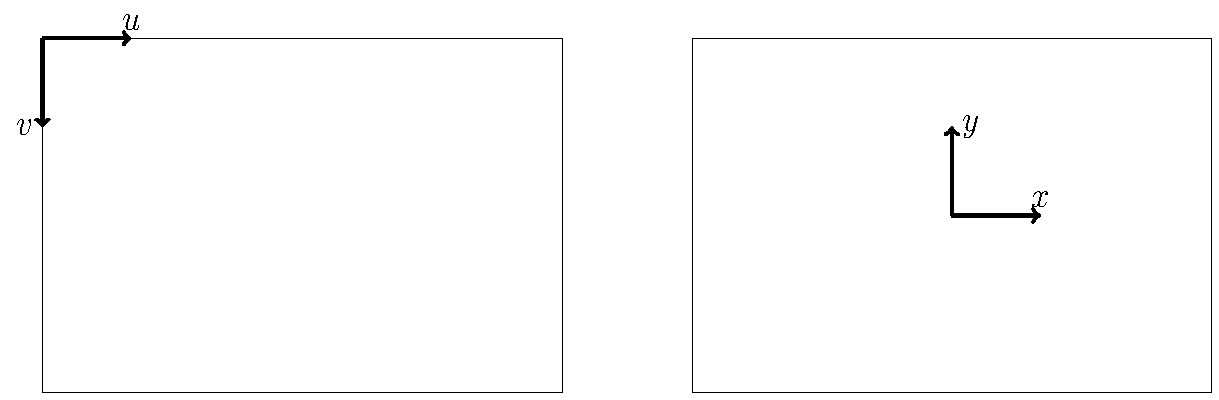
\includegraphics[width = \textwidth]{Figures/camera_coordinate_frame.pdf}
    \caption{Camera frame of reference}
    \label{fig:img_FOR}
\end{figure}

All frames read by the OpenCV library are images which follow the $uv$ frame of reference presented in Figure \ref{fig:img_FOR}. In order to apply the extrinsic parameters (which is explained in a later section) on certain points of the image, a frame of reference conversion is required. Extrinsic parameters and the transformation from 2D to 3D are applied on an $xy$ frame of reference similar to the one presented in Figure \ref{fig:img_FOR}. Once in 3D, the points will be expressed in the $XYZ$ frame of reference presented in Figure \ref{fig:vehicle_FOR}.

\begin{figure}[H]
    \centering
    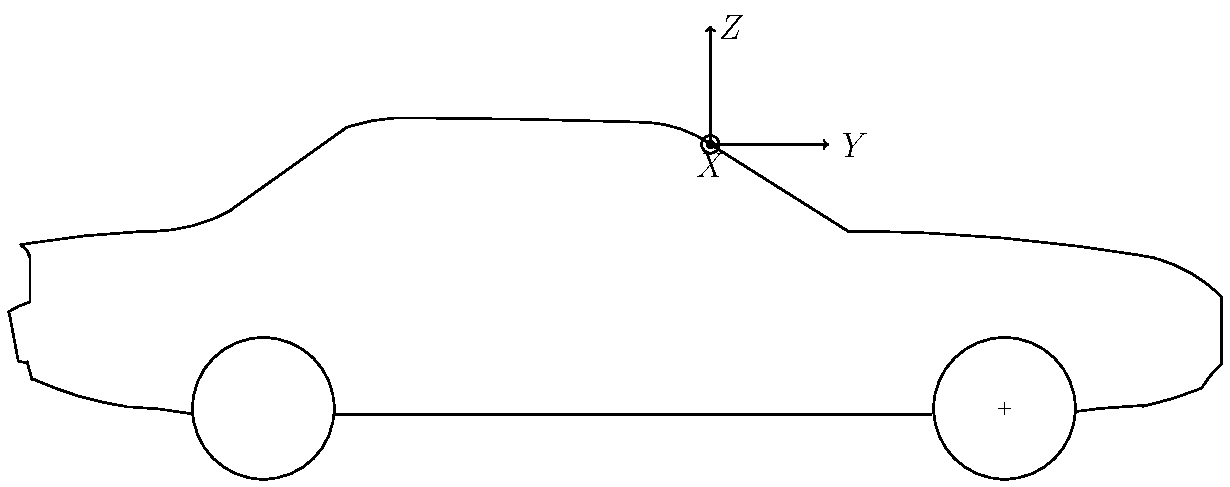
\includegraphics[width = 0.8\textwidth]{Figures/V_FBD.pdf}
    \caption{Vehicle frame of reference}
    \label{fig:vehicle_FOR}
\end{figure}



\subsubsection{Intrinsic Parameters}
The intrinsic parameters in this project are limited to the radial and tangential distortions which are explained in the literature review and in \cite{wang2008new}. For rectifying an image using the OpenCV library, the camera matrix and an array of distortion coefficients are required as an input. The camera matrix is defined by its focal lengths and the coordinates of its principal center which are provided from VTTI such that
\begin{equation}
    A = 
     \begin{bmatrix}
    f_u & 0 & c_x\\
    0 & f_v & c_y\\
    0 & 0 & 1
    \end{bmatrix}
\end{equation}
where
\begin{equation}
    f = 
     \begin{bmatrix}
    f_u \\ f_v
    \end{bmatrix}
    =
    \begin{bmatrix}
    347.1960 \\ 352.3415
    \end{bmatrix}
\end{equation}

\begin{equation}
    c = 
    \begin{bmatrix}
    c_x \\ c_y
    \end{bmatrix}
    =
    \begin{bmatrix}
    241.5788 \\ 188.9012
    \end{bmatrix}
\end{equation}
The array of distortion coefficients is expressed as

\begin{equation}
    DistortionCoefficients = 
    \begin{bmatrix}
    k_1 ~~ k_2 ~~ p_1 ~~ p_2 ~~ k_3
    \end{bmatrix}
\end{equation}
where $k_1,k_2 ~ and ~ k_3$ are radial distortion coefficients, and $p_1~and~p_2$ are tangential distortion coefficients. Those coefficients are acquired from VTTI. The array used for the rectification is hence

\begin{equation}
    DistortionCoefficients = 
    \begin{bmatrix}
    -0.432387 ~~ 0.183867 ~~ -0.038207 ~~ 0.000657 ~~ 0.000187 
    \end{bmatrix}
\end{equation}

It is important to keep in mind that not all videos in the database are recorded using the same camera. This means that using those distortion coefficients for all the videos is one of the assumptions in the project.


\subsubsection{Extrinsic Parameters}
\label{sec:meth_ExtrensicParameters}

Any point $(x',y')$ in the $xy$ image frame can be rectified with the extrinsic parameters to a point $(x,y)$ which can be used for further processing and distance calculation later on. This can be seen in Figure \ref{fig:homo_rect} where point $p$ has the coordinates $(x,y)$ after the rectification is applied to point $p'$. 
\begin{figure}[H]
    \centering
    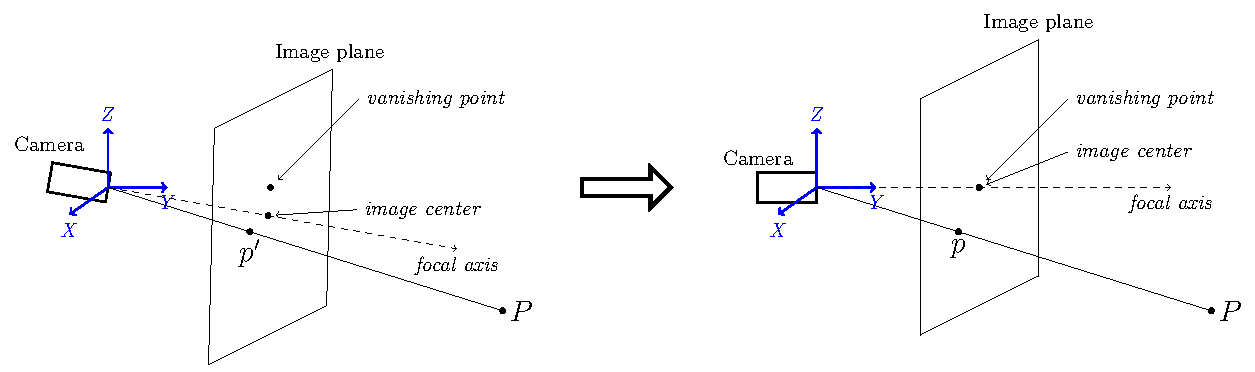
\includegraphics[width = \textwidth]{Figures/homo_rectify.pdf}
    \caption{Rectifying the camera's extrinsic parameters with homography}
    \label{fig:homo_rect}
\end{figure}

This rectification is interpreted as a transformation matrix called the homography matrix $\bf{H}$. The homography matrix is in general a relation between two images of the same object taken from a different camera or pose. In this case, the different camera poses are of the same dashcam before and after accounting for the extrinsic parameters which are the pitch and yaw of the SV. The theory of this transformation matrix is described here. A point $(x',y')$ is transformed to $(x,y)$ using the homography matrix $\bf{H}$.

\begin{equation}
    \begin{bmatrix}
    lx\\ly\\l
    \end{bmatrix}
    = \bf{H}
    \begin{bmatrix}
    x' \\ y' \\ 1
    \end{bmatrix}
    = 
    \begin{bmatrix}
    r_{11} & r_{12} & f_u r_{13}\\
    r_{21} & r_{22} & f_v r_{23}\\
    \frac{r_{31}}{f_u} & \frac{r_{32}}{f_v} & r_{33}
    \end{bmatrix}
    \begin{bmatrix}
    x' \\ y' \\ 1
    \end{bmatrix}
\end{equation}
where the $l$ is an arbitrary scaling factor and the components $r_{i,j}$ form the \textit{Euler-Rodrigues rotation matrix} \cite{DAI2015144} which states
\begin{equation}
    {\bf R} = {\bf I} + \left( sin \alpha \right) {\bf J_v} + \left( 1 - cos \alpha \right) {\bf J_v^2} = r(i,j)
\end{equation}
where we will define $\alpha = \begin{Vmatrix} \Omega \end{Vmatrix}$,  $\Omega = (\theta, \phi, \psi)$, $\textbf{v} = (v_x,v_y,v_z) = \frac{\Omega}{\alpha}$, and \textbf{$J_v$} is a skew-symmetric matrix defined as
\begin{equation}
\bf{J_v} = 
\begin{pmatrix}
0 & -v_z & v_y \\
v_z & 0 & -v_x \\
-v_y & v_x & 0
\end{pmatrix}    
\end{equation}

\begin{equation}
{\bf R} \approx {\bf I} + 
\begin{bmatrix}
0 & \phi & -\psi \\
-\phi & 0 & \theta \\
\psi & -\theta & 0
\end{bmatrix} =
\begin{bmatrix}
1 & \phi & -\psi \\
-\phi & 1 & \theta \\
\psi & -\theta & 1
\end{bmatrix}    
\end{equation}
Here, the angles $\theta, ~ \psi ~ and ~ \phi$ are the camera's pitch, yaw and roll angles respectively. So the homography matrix becomes

\begin{equation}
\bf{H} = 
\begin{bmatrix}
1 & \phi & -f_u \psi \\
-\phi & 1 & f_v \theta \\
\frac{\psi}{f_u} & -\frac{\theta}{f_v} & 1
\end{bmatrix}     
\end{equation}

In this project, it is assumed that the roll angle $\phi$ of the vehicle is negligible. Since the camera and the SV are assumed to share the same angels, the homography matrix narrows down to

\begin{equation}
\bf{H} = 
\begin{bmatrix}
1 & 0 & -f_u \psi \\
0 & 1 & f_v \theta \\
\frac{\psi}{f_u} & -\frac{\theta}{f_v} & 1
\end{bmatrix}   
\end{equation}

In order to get the pitch and yaw angles ($\theta$ and $\psi$), the vanishing point method will be used. In an image plane, all lines lying on one plane and parallel to each other will meet at a point called the vanishing point. Considering the ground plane, this means that parallel lane lines will intersect at a certain vanishing point in the image plane. In 3D, this point has a coordinate $Y=\infty$, meaning it is on the horizon. Joining all parallel lines of different slopes together will eventually create a set of vanishing points which, if joined, make up the horizon (also referred to as vanishing line) \cite{WANG2004}.

Finding the vanishing point in the image plane is a straight forward task. Whether it is by automatic lane detection, or by manually selecting points on the lane lines, an equation of each lane line can be developed. The vanishing point is then the intersection of those two lines. Considering two points on each lane, where points $(x_{11},y_{11})$ and $(x_{12},y_{12})$ are on one line, and $(x_{21},y_{21})$ and $(x_{22},y_{22})$ are on the other, the coordinates of the vanishing point become:
\begin{align}
    x_{vp} &= \frac{b_2-b_1}{m_1-m_2},\\
    y_{vp} &= m_1 x_{vp} + b_1
\end{align}
where each line has an equation $y = mx + b$, $m$ is the slope of the lane line and $b$ is the y-intercept.
% Show a figure.

Now from the location of the vanishing point in relation to the centre of the image, the pitch and yaw can be estimated, and the homography matrix can be created that for the vanishing point $vp$ as follows:
\begin{align}
    0 &= x_{vp} + f_u \psi\\
    0 &= y_{vp} + f_v \theta
\end{align}
This can be assumed since the mapping of the vanishing point using $\bf{H}$ should give a zero vector. Hence, the pitch and yaw angles are calculated as:
\begin{align}
    \psi &= \frac{-x_{vp}}{f_u}\\
    \theta &= \frac{-y_{vp}}{f_v}
\end{align}
\subsection{Lane Tracking}

To be able to calculate the distance between the POV and the lane, the lane has to be found in the video frame by frame. This could be done manually by the user or automatically by a software. The first option is easier to implement in a tool, but is a time-consuming task for the user. The second option is more demanding to implement, but if done correctly, could speed up the annotation process and provide more data to be used for analysing and model driver behaviour. The development process of the two lane detection methods, manual tracking and automatic tracking, are presented in this section.  

\subsubsection{Manual Tracking}

In this method, the lanes are defined manually by the user through marking points on the left and the right lanes in the video frames. The coordinates of these points were then used to calculate a linear line through the aforementioned points. To speed up this process, the user can define the lanes in one frame (possibly, the initial frame), skip through multiple frames, and define the lanes again (possibly, in the last frame). The program will then interpolate the lane placement and draw a an approximation of the lane placement on every frame between these two frames. The user will now be able to view all the frames with the drawn approximated lane and make changes in the markings of the points if the approximation of the lane position is not correct. 


\subsubsection{Automatic Tracking}
The aim was to develop a robust lane detection algorithm that required little manual work from the user. Robust in this case means that the lane detection should work well with both low and high quality NDS videos. Also, it should work well on videos recorded both during the day and during the night. All the steps involved in the development process of the lane detection algorithm are described below. An important remark is that  the algorithm is based on the one described in the literature review, section 1.3.2, but different approaches were tested in order to make the lane detection as good as possible. Three different definitions of region of interest was tested, this is presented later in this section. Also, Four different colour scales were tested, which are also presented later in this section. 

An overview of the developed automatic lane detection algorithm is presented in figure \ref{fig:my_label}. All steps in the development process of the algorithm are described below.

\begin{figure}[H]
    \centering
    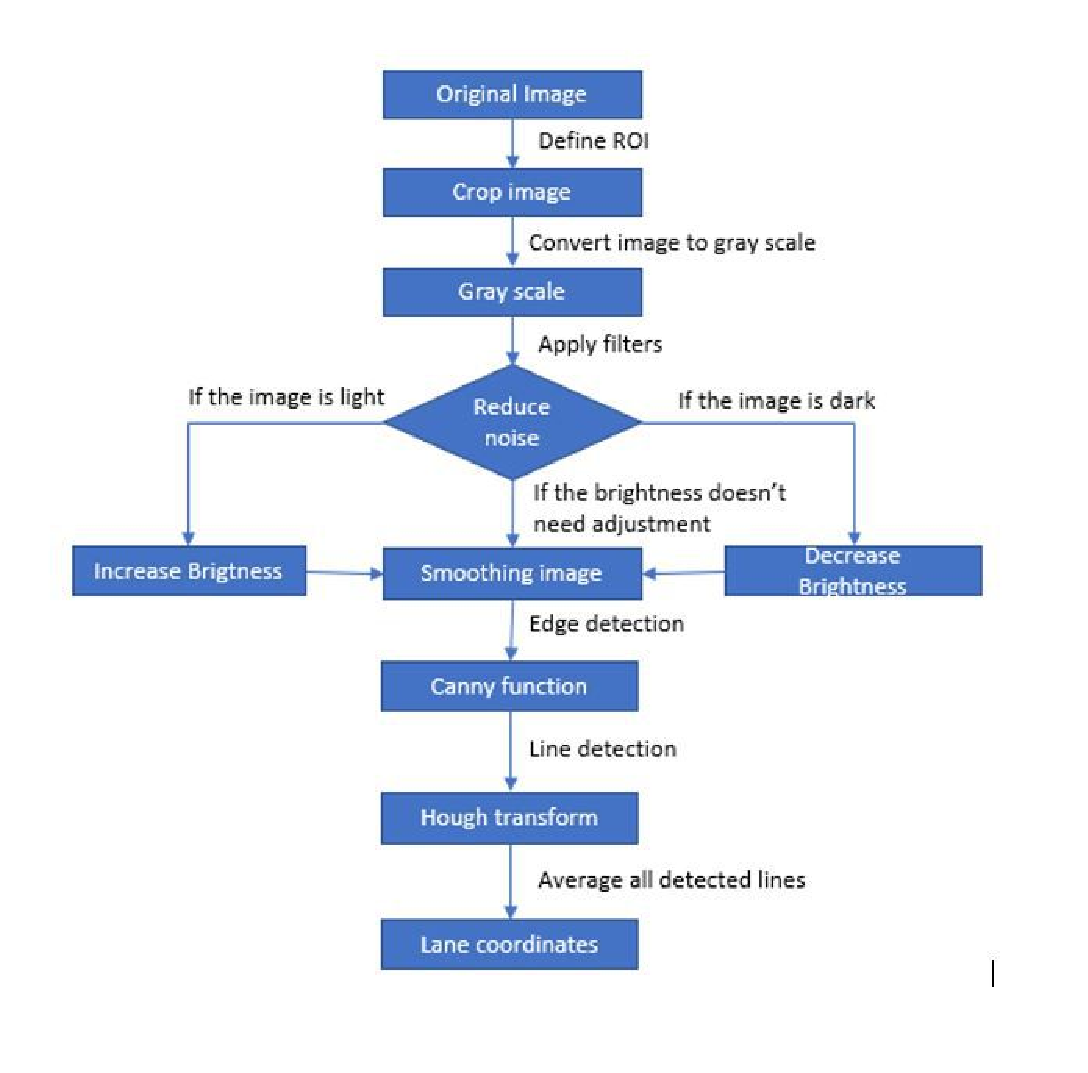
\includegraphics[width=\textwidth]{Figures/Algorithm.pdf}
    \caption{Final algorithm based on results obtained after masking}
    \label{fig:my_label}
\end{figure}

\paragraph{Region of Interest}

The first thing to do in order to detect the lanes in one frame is to define the Region Of Interest (ROI). The ROI contains all the interesting information in an image, in this case the area where the lanes are, and ensure that all the unnecessary information is ignored. A well-defined ROI contains as little unnecessary information (such as the landscape around the road, the road shoulders and other vehicles) as possible. Since the aim is to make the lane detection as automatic as possible, the ROI needs to be define with as little user input as possible. The different ROI:s that were considered for the algorithm are described below, together with their respective pros and cons.

\subsubsection*{ROI 1: Lower half of the image}
The ROI is defined as the bottom half of the image, like the region in red marking in Figure \ref{fig:my_ROI}. The positive aspect of this ROI is that the user doesn’t need to manually define the ROI. However, the ROI will contain a lot of unnecessary information, such as the landscape around the road, the road shoulders and the road between the lanes. This will lead to problems later when its time to detect the lanes. 

\subsubsection*{ROI 2: Triangular shape}
The ROI is defined as a triangle that contains the whole road, like the region in black marking in Figure \ref{fig:my_ROI}. This ROI needs to be defined by the user in the beginning of the annotation for the first frame, but the same ROI can be used in the upcoming frames. Assumed that the road doesn’t have any sharp turning during the event of interest, the same ROI can be used for the whole video.

\subsubsection*{ROI 3: Focus on one lane}
The ROI is defined as a small rectangle that mainly contains one of the lanes, like the region in blue marking in Figure \ref{fig:my_ROI}. This ROI needs to be defined by the user for at least two frames, the idea is that the user defines a ROI for the first frame and then define a new ROI for a frame a couple of time steps later. The ROI is then interpolated between the two frames and automatically updated for every frame. The number of frames for which the interpolation  can be applied depends on the shape of the road. If the road has a sharp turn, the user needs to define the ROI for more frames compared to a relative straight road. Also, the user needs to define one ROI for both the left and the right lane. This type of ROI consist of little unnecessary information, which will be helpful later when it is time to detect the lanes.

After trying all three types of ROI, the ROI focused on one lane successfully detected the most number of lanes and is therefore then one used in the lane detection algorithm.



\begin{figure}[H]
    \centering
    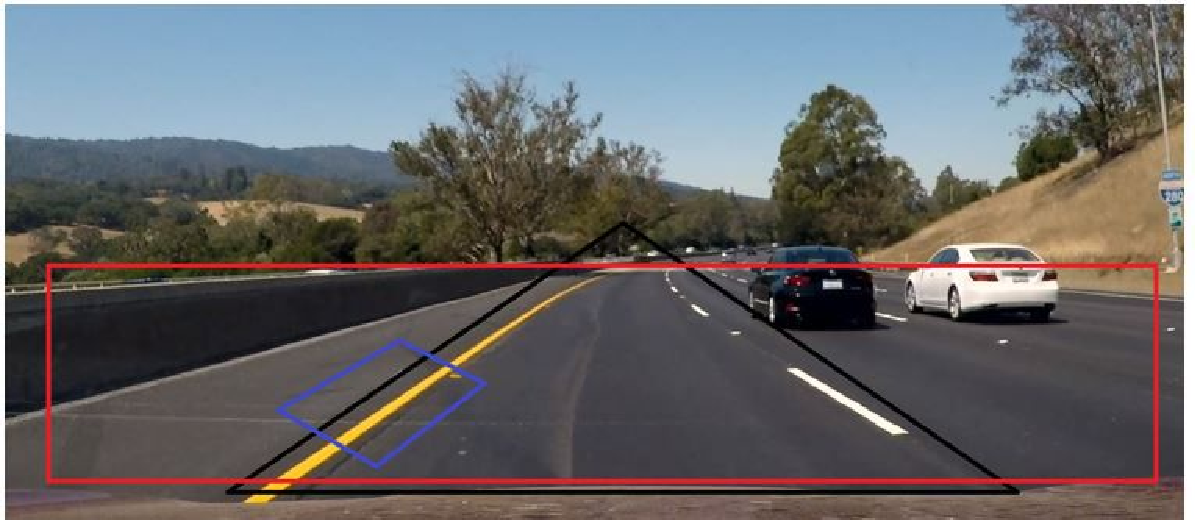
\includegraphics[width = 0.6\textwidth]{Figures/ROI_new.pdf}
    \caption{Approach to selecting different Region of interest}
    \label{fig:my_ROI}
\end{figure}

\paragraph{Colour selection}

The next step is to detect all the edges of lanes in the defined ROI for all the frames. As described in the literature review, section 1.3.2, the edges in an image is found by looking at the rapid change in intensity from two adjacent pixels. The intensity can be amplified and therefor make the edges more easy to detect by using different colour scales and mask out certain colours. In this case, the boundary of the yellow or white lanes and the gray asphalt is what defines the lanes and should be detected. The sections below describe different colour scales and how effective they are in amplifying the pixel intensity.

\subsubsection*{Color selection: Grayscale}
It is easy for the human eye to differentiate the gray asphalt from the yellow or white lanes, but due to shadows, complex lightning and worn out lanes (which change the pixels intensity on the road), it can be hard for a computer to distinct between the white/yellow lane and the road surface. Using a grayscale filter to convert the original RGB image to an image which consist of different shades of gray will reduce the shadows and lightning's influence and hence make the distinction between lanes and road surface clearer. Figure \ref{fig:color_scale} (top right) shows the original image after a grayscale filter been applied.

\subsubsection*{Color selection: Colour scales}
An alternative method to detect lanes is to filter out all the colours in the image except for the colours that the lane has, namely yellow and white. Different colour scales have different colour contrast, and a higher colour contrast makes it easier for a computer to detect a certain object with a certain colour. The different colour scales which was investigated during this work was RGB, HSV and HSL.  The original RGB image, which can be seen in figure \ref{fig:color_scale} (top left) was converted to a HSV image and HSL image, shown in figure \ref{fig:color_scale} (bottom right and bottom left respectively). The threshold values for yellow masking and white masking for the different colour scales are shown in table \ref{tab:Colour_conversion}. 

\begin{table}[H]
    \centering
    \begin{tabular}{c|c|c|c|c}
         \multicolumn{5}{c}{\textbf{Colour conversion}} \\ \hline
         Colour scale & Lower white & Upper white & Lower yellow & Upper yellow \\ \hline
         RGB & 160, 160, 160 & 255, 255, 255  & 150, 150, 0  & 255, 255, 80\\
         HSV & 0, 0, 160 & 0, 0, 255  & 60, 255, 150  & 60, 175, 255 \\
         HSL & 0, 0, 160 & 0, 0, 255  & 60, 255, 75  & 60, 255, 170
    \end{tabular}
    \caption{Threshold for yellow and white masking for different colour scales}
    \label{tab:Colour_conversion}
\end{table}


\begin{figure}[H]
    \centering
    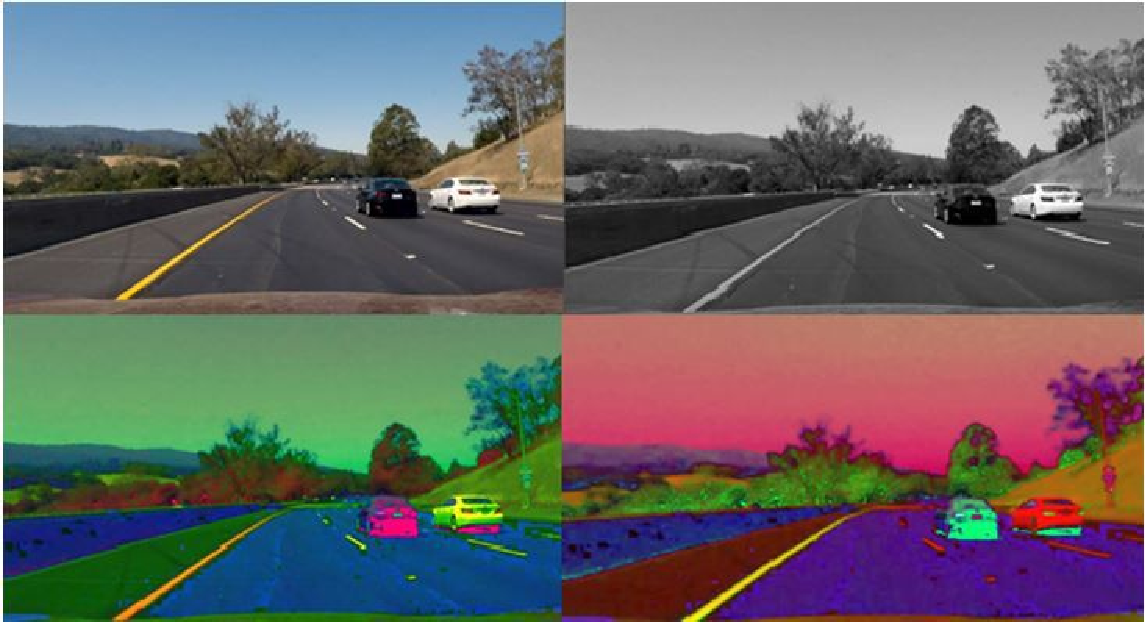
\includegraphics[width = 0.8\textwidth]{Figures/colorscale_2.pdf}
    \caption{Image conversion on different color scale}
    \label{fig:color_scale}
\end{figure}

\paragraph{Filters}
In order to obtain a correct detection of objects in an image, it is first necessary to distinguish them correctly. The noise and details in an image are reduced using a well known filter called Gaussian filter. The Gaussian filter is simple as it requires varying only one parameter; the variance. As seen in the equation below, it can be inferred that the amount of filtering is inversely proportional to the variance. Based on the level of suppression required on an image, the respective variance can be applied.
Other filters that can be considered are the mean-average and the median filters. Although they work well in reducing noise in an image faster than the Gaussian filter, they are ineffective in identifying the rate of change of frequency in an image which has sharp changes in colour.

\begin{equation} 
G(x,y)= \frac{1}{2\pi \sigma^2} e^ \frac{-x^2+y^2}{2\sigma^2}
\end{equation}
If the frame in which the lanes shall be detected is taken during night time, or if there are strong shadows in the frame, the brightness needs to be increased for better lane detection. And in the same way if the frame is taken during strong sunlight, the brightness needs to be decreased. The brightness and contrast of an image can be adjusted by applying a filter. In figure \ref{fig:lighter}, a filter is applied to the original dark frame, figure \ref{fig:lighter} (left), so the frame gets brighter, figure \ref{fig:lighter} (right), and therefor the lanes gets more visible. In figure \ref{fig:darker}, a filter is applied to the original light frame, figure \ref{fig:darker} (left), so the frame gets darker, figure \ref{fig:darker} (right), and therefor the lanes gets more visible.

\begin{figure}[H]
    \centering
    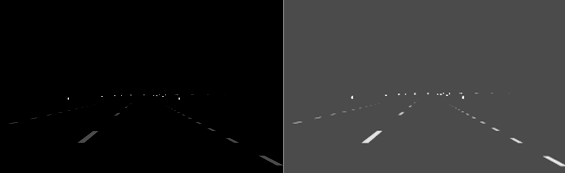
\includegraphics[width = 0.8\textwidth]{Figures/lighter.png}
    \caption{Increase the brightness of an image with a filter}
    \label{fig:lighter}
\end{figure}


\begin{figure}[H]
    \centering
    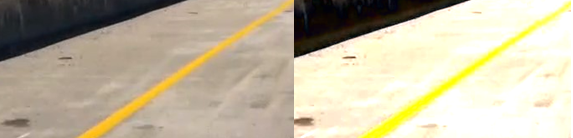
\includegraphics[width = 0.8\textwidth]{Figures/darker.png}
    \caption{Decrease the brightness of an image with a filter}
    \label{fig:darker}
\end{figure}


\paragraph{Canny edge detection}

The edges in the defined ROI are now ready to be detected. The edge detection is done with a canny function. The canny function was applied to all three different colour scales frames and the gray scale frame presented in figure \ref{fig:color_scale} and the result is presented in figure \ref{fig:canny}. The canny function applied to the original RGB image can be seen in figure \ref{fig:canny} (top left). The canny function applied to the converted HSV image and the converted HSL image can be seen in figure \ref{fig:canny} (bottom right and bottom left respectively). Finally, the canny function applied to the gray scale image can be seen in figure \ref{fig:canny} (top right).


\begin{figure}[H]
    \centering
    
\includegraphics[width = 0.8\textwidth]{Figures/edge.pdf}
    \caption{Edge detection using canny operator}
    \label{fig:canny}
\end{figure}

\paragraph{Hough Transform}
\label{par:Hough_t}
Hough transform is a widely used  technique in computer vision and image analysis for feature extraction. Originally, it was used to identify lines but later was developed for other shapes as well. 
\begin{figure}[H]
    \centering
    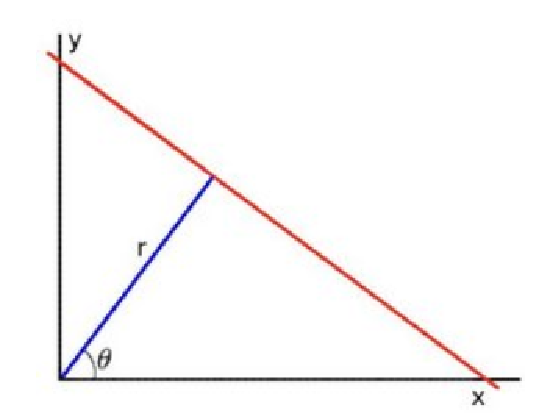
\includegraphics[width = 0.4\textwidth]{Figures/line_pol.pdf}
    \caption{A line in polar co-ordinates}
    \label{fig:Hough}
\end{figure}
Considering the equation of a line in polar co-ordinate system from Figure \ref{fig:Hough}, where $r$ represents the perpendicular distance to the line, ($\theta$) is the angle in radians with the X-axis and (x,y) are points on line for which $r$ and $\theta$ are constants.
\begin{equation}
    r = x cos(\theta) + y sin(\theta)
    \label{eq:Hough_eq}
\end{equation}
Since the variables (r,$\theta$) of the equation of line have to lie between definite values, the equation of line in Cartesian form can not be used as slope may take values up to infinity.
From the equation \ref{eq:Hough_eq},it can be inferred that for known points (x,y), the subsequent (r,$\theta$) can be plotted. Each point gives a sinusoidal curve in the (r,$\theta$) plane.The points which are collinear yield curves which intersect at common point (r,$\theta$)  This essentially forms the principle behind the Hough transform. The threshold can be set for the number of lines which intersect ar r and $\theta$. The Hough transform declares a line based on the set threshold. 



\paragraph{Averaging lines}
As seen in section \ref{par:Hough_t}, the Hough transform is used to identify which of the detected edges are part of a lane and reject those edges that are not part of a lane.  In the ideal case, the Hough transform identify two edges as parts of a lane, the vertical left and right side of the actual lane. The detected lanes position is estimated by taking the average slope and the average position in x,y- coordinates of the detected edges. In some cases however, the Hough transform misdetect an edge as part of a lane, which will lead to a worse estimation of the lanes position. In order to avoid misdetection of lanes, the algorithm only consider the edges which have a similar slope, that is maximum 60 degrees different, to the region of interest.  

The estimated lanes are drawn on the frame which are analysed so the user can visually determine if the estimation is accurate. Also, the estimated lanes end-points in x,y-coordinates are given as an output from the algorithm




\paragraph{Bird's eye perspective}
The image obtained from forward facing camera appears to converge to an infinite point in the image plane due to perspective. It is vital to correct this as it affects the parameters to be calculated. To change the perspective as viewed from the top gives a better understanding of the lanes, especially the curved ones.

The most commonly used technique is bird's eye transformation. This allows the image to be transformed such that it appears as seen from the top. This method could be an alternative to solving the heading angle problem. However, it's limitation is that only lanes are seen clearly where as objects are stretched in the vertical direction and may not useful in annotating cars. 


\subsubsection{Semi Automatic Tracking}
This method will let the user define the Region Of Interest in a couple of frames, then the lane detection algorithm described above could search for the lanes within this RIO. This would allow for faster annotation compared to manual annotation and better lane detection. 

\subsubsection{Test of Lane detection algorithm}

Some tests was performed in order to determine which of the colour scales gives the best result in terms of detecting lanes and should therefor be used in the final lane detection algorithm described in section 2.2.2. The four different colour scales, namely RGB, HSV, HSL and gray scale was tested on three different scenarios, NDS videos containing dashed lanes, NDS videos containing solid lanes and NDS videos recorded during night time. Three representative videos were used for each of the three scenarios and the results are presented in section 3.2. 

In order to check how trustworthy the lane detection algorithm is in the sense that the detected lanes are actually lanes and not something else, a misdetection test was performed. In the test, the ROI of the lane detection algorithm was defined in an area of the frame where no lanes are present, and the percentage of misdetected lanes was noted. The test was done both for videos recorded both during day time and videos recorded during night time. The results of this test are presented in section 3.2.

In order to check how accurate the lane detection are, a flickering test was performed. Flickering is the relative horizontal movement in pixels of the detected lane from one frame to the next frame. Lanes are used as an measuring rod for the vehicles position on the road, and high flickering creates the false impression the the vehicle has a lateral movement. The flickering test was performed for one NDS video recorded during day time and one NDS video recorded during day time and the result is presented in section 3.2.



\subsection{Heading Angle}
The heading angle is one of the parameters of interest for the project, partly because it is relevant in the development of the driver model, and partly because it helps enhance the other calculations that will follow (i.e. lateral offset and longitudinal range). Three methods for calculating the heading angle are introduced here, although only the first method is used for the development of the tool.

\subsubsection{Method 1 for Heading Angle: Triangulation}
After identifying the vanishing point and rectifying the image for intrinsic and extrinsic parameters, one can transform points on the picture from the 2D view to a 3D view, as long as one of the coordinates is known. For the sake of this project, the transformations will be on the ground plane, meaning that the Z-component of the points to be calculated is known and equal to the height of the camera above the ground. The following figure depicts what is meant by transforming the view from 2D to 3D coordinates.

\begin{figure}[H]
    \centering
    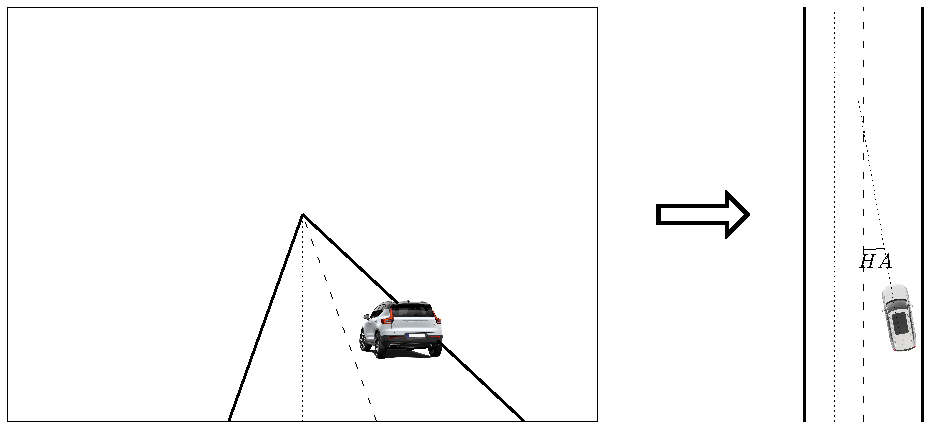
\includegraphics[width=\textwidth]{Figures/2d2d3.pdf}
    \caption{2D to 3D transformation}
    \label{fig:2d23d}
\end{figure}


In order to change from 2D to 3D coordinates, the following method can be used starting with calculating the Y-coordinate (longitudinal distance) of a ground point and then its X-coordinate) lateral offset.

\begin{figure}[H]
    \centering
    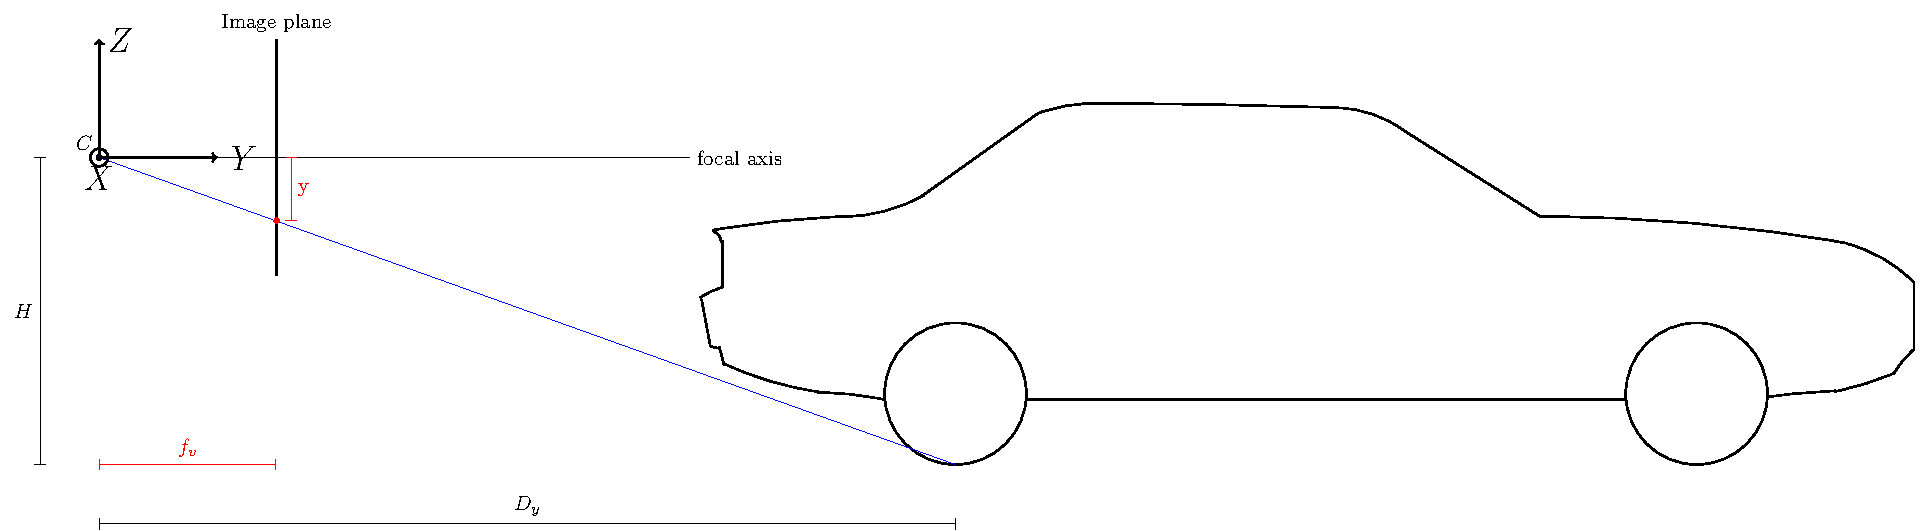
\includegraphics[width=\textwidth]{Figures/D_y.pdf}
    \caption{Distance calculation in $yz$-plane of vehicle reference frame}
    % \label{fig:my_label}
\end{figure}

\begin{equation}
    \frac{D_y}{H} = \frac{f_v}{y} \Rightarrow D_y = \frac{H f_v}{y}
\end{equation}



\begin{figure}[H]
    \centering
    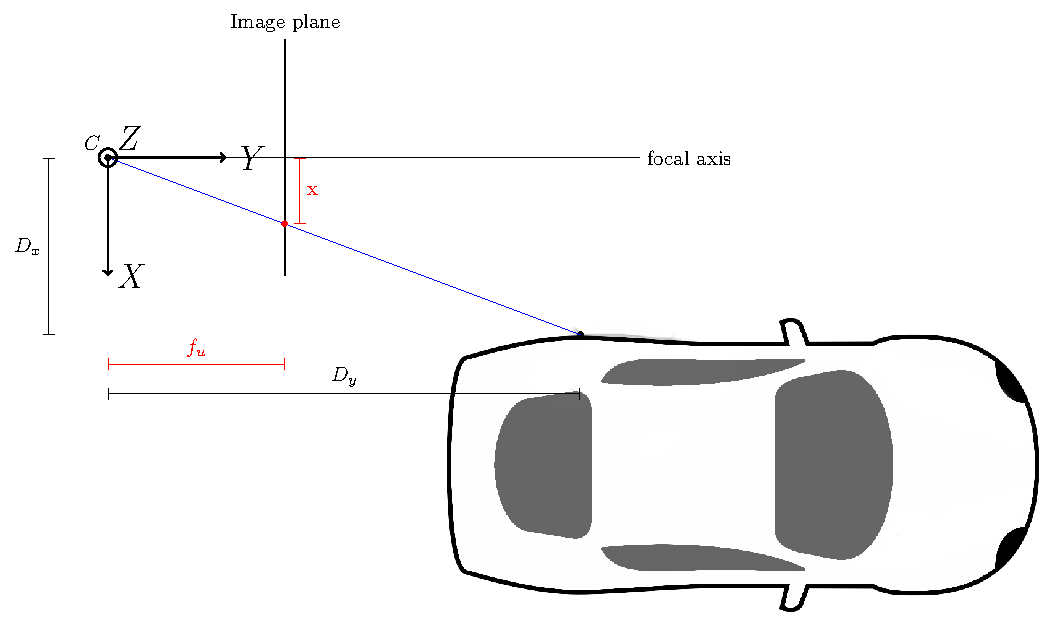
\includegraphics[width=\textwidth]{Figures/D_x.pdf}
    \caption{Distance calculation in $xy$-plane of vehicle reference frame}
    % \label{fig:my_label}
\end{figure}

\begin{equation}
    \frac{D_y}{D_x} = \frac{f_u}{x} \Rightarrow D_x = \frac{D_y x}{f_u} = \frac{H f_v x}{f_u y}
\end{equation}

The coordinates in 3D of the wheels can now be expressed as
\begin{equation*}
    \begin{bmatrix}
    X\\Y\\Z
    \end{bmatrix}
    =
    \begin{bmatrix}
    D_x\\D_y\\-H_{camera}
    \end{bmatrix}
\end{equation*}

Using the X and Y coordinates of the two wheels, one can get the equation of the line joining the two wheels and by getting the slope of this line one can easily calculate the heading angle of the POV. The heading angle is hence

\begin{equation}
    HA = \psi_{POV} = -tan^{-1} \left( \frac{X_1 - X_2}{Y_1 - Y_2} \right)
\end{equation}

\subsubsection{Method 2 for Heading Angle: Number plate}
This method is suggested by the team members but not used in the project. It was also not found to be used in other research either. The method can be described as follows: using the number plate of a car, which has a standard shape and size, one can check the edges of the plate and calculate the size and angles shown in the picture. Based on that, one can get the heading angle of the vehicle. This method may not be the best way to follow, due to the limited quality of the videos available in the dataset.

\subsubsection{Method 3 for Heading Angle: Side plane homography}
This method is also based on the homography concept. By checking the change in the homography of the side of the car and tracking this plane as the car moves, one can achieve the rotation of this plane relative to the camera and hence the relative heading angle of the POV. This method has several difficulties, especially the translation of the camera, and is to be investigated in future work.

\subsection{Lateral Offset}
The lateral offset is another important parameter for developing a driver model. In fact, the lateral distance to the lane marking and the "speed of attack" of the POV towards the lane line are of paramount interest in this project. Two methods for estimating the lateral offset of the POV are discussed here.

\subsubsection{Method 1 for Lateral Offset: Pixel width}
Using the pixel size of the rear end of the vehicle, one can get the distance from the center of the vehicle to the focal axis of the camera. This is solved by a system of 2 equations where the unknown variables are the lateral offset $L$ and the range of the car $D$.

\begin{figure}[H]
    \centering
    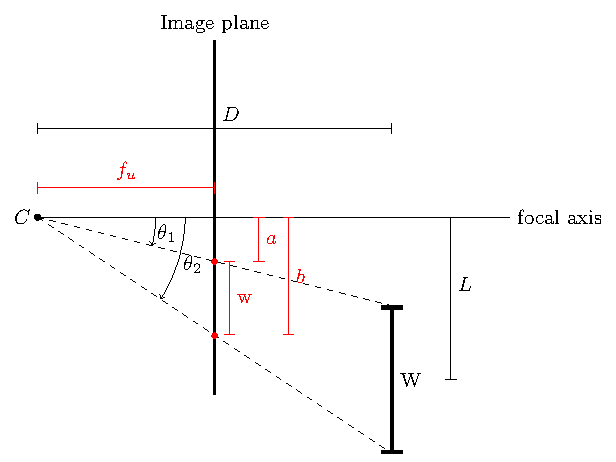
\includegraphics[width = 0.8\textwidth]{Figures/DistanceCalc.pdf}
    \caption{Distance calculation using pixel width method}
    % \label{fig:my_label}
\end{figure}

\begin{equation}
    \frac{a}{f_u} = tan\left( \theta_1 \right) =  \frac{L - \frac{W}{2}}{D} \label{eq:dista}
\end{equation}
\begin{equation}
    \frac{b}{f_u} = tan\left( \theta_2 \right) = \frac{L + \frac{W}{2}}{D} \label{eq:distb}
\end{equation}

By solving the system of equations above, we get the following results:
\begin{equation}
    D = \frac{W f_u}{b-a} \label{eqn:distD}
\end{equation}
\begin{equation}
    L = \frac{W}{2} \left( \frac{a+b}{b-a}\right) \label{eqn:distL}
\end{equation}

In some cases, the POV will have a certain heading angle, which will cause the pixel width $w = b-a$ to seem smaller than what it is in reality. To account for that, the heading angle should be incorporated in the pixel width $w$ such that
\begin{equation}
    w' = \frac{w}{cos(\psi_{POV})} \label{eqn:w_withheading}
\end{equation}

It is important to note that this method gives the relative distances of the POV with respect to the camera's center. In order to get the lateral offset of the POV to the lane, further development of this method is required where the position of the SV in its lane in known.

\subsubsection{Method 2 for Lateral Offset: Triangulation}
Using a similar approach to what was explained earlier, one can get the 3D coordinates of the contact between the wheels and the ground ($X_w,Y_w,Z_w$). Also, getting the equation of the lane line in 3D follows the same method. With the wheel coordinates and the lane line equation in hand, it becomes simple to get the distance between the wheels and the lane. This approach is in fact a simple 2D calculation since all the points lie on the ground plane. The equation used to get the distance between the points and the lane line is:
\begin{equation}
    lateralDistance = \frac{m X_w - Y_w + b}{\sqrt{a^2+1}}
\end{equation}
where the equation of the lane line in the ground plane is $Y = mX+b$.

By deriving the resultant distance with respect to time (i.e. dividing the change in the lateral distance by the time step of each frame), the lateral offset speed and the "speed of attack" of the POV towards the lane line are obtained.

\subsubsection{Error Estimation}
The two methods mentioned above rely on assumptions that affect the accuracy and precision of the results. To check the performance of the tool, the resultant distances will be compared to radar data that is available for the dataset in hand. The errors are hence calculated based on the difference between the output of the tool and the radar data.

Those errors are caused by the following assumptions:
\begin{itemize}
    \item Width of POV
    \item Length of trunk of POV
    \item Camera's height
    \item SV's hood length
    \item Extrinsic parameters (pitch and yaw angles of camera)
    \item Manual selection of the POV's rear and wheels as well as the manual selection of points on the lane lines
    \item Interpolation between frames
\end{itemize}


\subsection{Range Estimation}
For the estimation of the range between two vehicles, several methods are available. Two methods which are be implemented in this project are described here.

\subsubsection{Method 1 for Range Estimation: Pixel width}
The pixel width method, which is explained earlier, can be used for estimating the range between the two vehicles based on the number of pixels that the rear end of the POV encompasses on the image frame. The distance $D$ is calculated in Equation \ref{eqn:distD} which is derived earlier.

As mentioned earlier, the range estimation is enhanced by accounting for the heading angle of the POV as shown in Equation \ref{eqn:w_withheading}.

\subsubsection{Method 2 for Range Estimation: Triangulation}
This method has also been described before. For the sake of the range estimation, the tool will get the 3D coordinates of the rear left point of the POV, which lies on the ground. For this method to work properly, the used must be careful when defining the rear of the vehicle. While the pixel width method relies on the number of pixels which are estimated by the brake lights, this method assumes that the lower edge of the box defined by the user for the rear end of the POV is on the ground plane. Using this assumption, the tool will calculate the distance to the lower left corner of the user defined box.

Another way to get the range is to calculate the distance to the rear wheel, which was defined for calculating the heading angle, and account for the length of the POV's trunk.


\subsubsection{Error Estimation}
Similar to the estimation of lateral distances, the longitudinal distances also rely on the assumptions discussed earlier. For the same reason as before, an error will be calculated based on the difference between the output of the tool and the radar data available.
\subsection{Vehicle Tracking}
To be able to calculate the speed and the distance to the POV, the width of the POV has to be found in video frame by frame. Like lane tracking, this could be done manually by the user, automatically by the program or in a semi-automatic fashion.

\subsubsection{Manual Tracking}
The user was asked to mark in the video image, frame by frame, where the rear of the POV is. Here, the rear of the vehicle is roughly defined by the two brake lights. To simplify this process, the user is given the option to define the rear of the POV in one frame, skip though multiple frames, then define the rear of the POV again in a later frame. The program will then interpolate the box coordinates between the user-defined inputs and estimate the width of the POV in the intermediate frames without any input from the user, in a similar manner to the manual lane tracking mentioned earlier. The user is then able to view all the video frames and make corrections where the estimations are not accurate (i.e the box is not bounding the rear of the POV). 

\subsubsection{Automatic Tracking}
The openCV library has some functions that can perform object tracking using pre-trained neural networks for identifying shapes in images. Depending on the quality of these algorithms, the POV could be identified in the video frames automatically. In that case, the user would only need to check the video images to assure that the automatic tracking has identified the POV correctly, through all the frames. 

\subsubsection{Semi-Automatic Tracking}
If the object tracker mentioned above is not accurate enough, one hybrid solution could be to combine the automatic tracker data with some user defined inputs, in order to make a more accurate estimation of the POV position across frames. This would have the benefit of reducing the time needed to annotate one video while maintaining good output quality.
\subsection{Design of Tool and Graphical User Interface}


The GUI should be intuitive and simple to use. The available input methods are the keyboard and mouse. These controls should be optimised to speed up the annotation process. The basic outline of the tool is described in the titles mentioned in this section.

\subsubsection{Video Player}
The video player must have the ability to load a video file from a chosen path and view it in a window. Since the goal is to annotate through the video and mark objects in the frames, the user should be able to play, pause and skip through frames.

The openCV library has a $imread()$ function that can read video files frame by frame and store them into arrays objects in the program memory. This would later allow for iterations through the video frames as well as drawing and marking objects on the frame by the user. The library also has an $imshow()$ function that can show the chosen image in a predefined window. These two functions will be used to develop the video player

\subsubsection{Controls}
The controls are what allow the user to control the video and mark objects in frames. This was done using keyboard buttons, where different keys were mapped to do different functions. Visual buttons were also added alongside the keyboard controls for better usability. 



Upon selecting a frame of interest, the user should be able to define an object in the frame. For this scope of this project, only the following objects were considered relevant for the intended output:

\begin{itemize}
    \item POV placement\\
    The user should select a rectangle in the part of the frame where the rear pf the POV is, since the range estimation will be calculated using the vehicle width in pixels. 
    \item POV wheels\\
    To be able to calculate the heading angle, the user should identify the points where the POV wheels touch the ground. 
    \item Right/Left lane\\
    The user should define points where the placements of the right and left lanes are.
\end{itemize}

For drawing and marking objects, the openCV library has a function to save the position and action of the computer mouse. These functions were used to draw shapes on the image to visualise user input. 

Keyboard controls were implemented using the openCV $waitkey()$ function that logs key presses while an OpenCV window is active. Upon pressing a key, a status variable would change within the program depending on which key was pressed. Visual control buttons with the same functionality were implemented in a separate window alongside the main view window using Tkinter and mapped to the same status variable. This way, both keyboard and visual buttons would work in tandem to improve usability. 

\subsubsection{Displaying Information}

It is important that the user sees areas that are marked and what the program has identified them as. This was done using different shapes and colours, alongside a window to display information to the user about the current status of the program (i.e what input is currently being saved). 

Different colours were implemented when drawing shapes in the image, using the openCV library. A separate window was implemented below the main view window using Tkinter, to display information about the current status of the program.

\subsubsection{Loading and Saving Data}
\label{sec:Loading_and_saving_data}

There are two inputs to the program, the video and the corresponding $.mat$ file containing the time-series data of the SV, which will be needed to calculate the output variables.

All the user input described above was saved in a structured manner that allows for ease of access within the program. This was done through creating a class with fields, much like a struct type in Matlab, that will be passed on as an argument to functions within the program. That way, the functions will have access to all available information, which was especially useful in the early testing and debugging phase. After the user is done with annotating a video, the data was saved to allow for re-annotation at a later time.

Two output files were created, first of which is a $.pickle$ file containing the annotation output. This file was exported using Pickle since it is easier to import the data back into Python as it maintains the structure and data types as the original object. The other is a $.mat$ file that contains the same data but is compatible with Matlab. This should make it easier for the annotator to post-process the data in Matlab, since it is a more familiar program for most and is the same type of file as the time-series data available from SHRP2. 


\subsubsection{Writing a User Manual}

After completion of the tool, a user manual was written to instruct the user on how to use the tool and some basic overview on the structure of the output data. This also includes guidelines on how to get better output accuracy.

\subsubsection{Testing User Sensitivity}
% \textcolor{red}{this part should be moved? the user annotation results were moved under the range estimation method 1}

% To verify the quality of the output data, some videos that have radar range available have been annotated using the tool. The output range in both lateral and longitudinal directions have been compared with the radar data available. This  provided an indication on the magnitude of the error between the annotated variables and the variables extracted from the SHRP2 dataset. 

To investigate how sensitive the tool is to the user input, a sample of videos were annotated by the four different members of the team multiple times, since not all annotators will input data identically. 


% The user interface will consist of a three main windows, one for viewing the chosen video, one for the control buttons, and one viewing information to the user about the current status of the program. The user will have the option to pause and  
% \input{Experiment}
%	Experiment and Results
\section{Results}
\label{sec:Results}
The results from the project are presented in this section. Note that all images of dash-cam footage presented below are not from the SHRP2 data since these cannot be shared and published. Instead, sample free to use videos were used to better show the findings in this section. However, the plots that are presented below were drawn using time-series data acquired from the SHRP2 data. 
% The time-series data used in this report 


\subsection{Image Rectification}
Both intrinsic and extrinsic image rectification were implemented. The results from the image rectification are shown below. 


\subsubsection{Rectification Using Intrinsic Parameters}

Initially, the video was rectified frame by frame using the intrinsic camera parameters. It is important to note that these parameters are camera specific and were acquired for the type of camera used to collect the SHRP2 data.

Figure \ref{fig:image_rectification} shows the result from this rectification on a sample image. Note that this image was resized to be the same resolution and aspect ratio as the videos in the SHRP2 data, hence the grey bars on the top and bottom. 

\begin{figure}[H]
\centering
\begin{minipage}[b]{0.45\linewidth}
    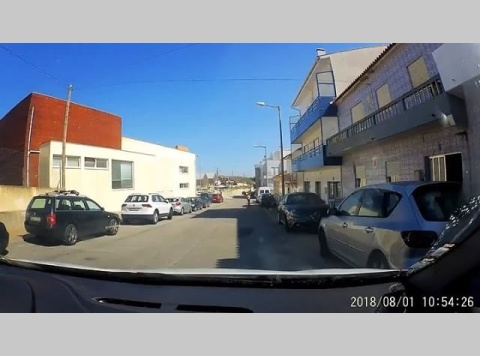
\includegraphics[width=\textwidth]{random_image_extended.jpg}
    \caption*{Distorted image}
\end{minipage}
\begin{minipage}[b]{0.45\linewidth}
    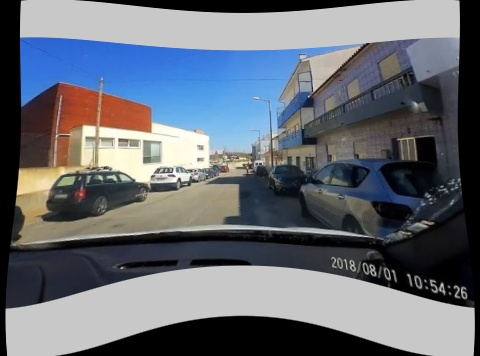
\includegraphics[width = \textwidth]{random_image_rectified.jpg}
    \caption*{Rectified image}
\end{minipage}
\caption{Image rectification using intrinsic parameters}
\label{fig:image_rectification}
\end{figure}

In figure \ref{fig:image_rectification}, it is apparent how the distorted image is stretched and straight objects, like poles, are not straight in the image. The rectification should correct that using the intrinsic parameters. This is not the case in the example presented, where the poles in the rectified image are still not completely straight. This is because the camera used in this example is not the same as the one used to collect the SHARP2 data, and should therefore have different intrinsic parameters.  


\subsubsection{Rectification Using Extrinsic Parameters}

In practice, if the extrinsic calibration is done correctly, then the VP of the lanes should always be moved to the centre of the image. This meant that if the VP is initially not at the centre of the image, the corresponding cam pitch and cam yaw were calculated and used as described in section \ref{sec:meth_ExtrensicParameters} to shift the VP so that it was at the same coordinates as the centre of the image, as shown in Figure \ref{fig:extrParamCali}. Note that only the VP is being transformed, hence the black background in the calibrated figure, which is only drawn to show the effects of the extrinsic calibration. 

\begin{figure}[H]
    \centering
    \begin{minipage}[b]{0.49\linewidth}
    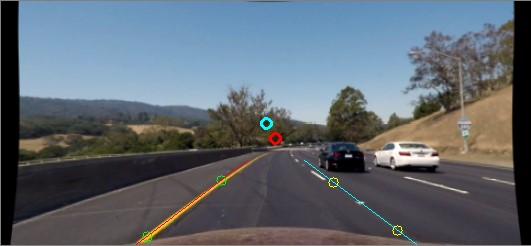
\includegraphics[width=\textwidth]{Figures/vp_initial.jpg}
    \caption*{points before calibration}
    \end{minipage}
    \begin{minipage}[b]{0.49\linewidth}
    
\includegraphics[width=\textwidth]{Figures/vp_fixed.jpg}
    \caption*{points after calibration}
    \end{minipage}
    
    \caption{Image rectification for extrinsic parameters (VP (red) and Image Centre (aqua))}
    \label{fig:extrParamCali}
\end{figure}

\subsection{Lane Tracking}

The three methods of lane tracking previously mentioned were studied. Manual tracking was easy to implement. Fully automatic tracking was more demanding and was not pursued due to the limited time frame of the project. However, semi-automatic was implemented. The results from all three methods are presented below. 
 
\subsubsection{Manual Tracking}

It was found that this method did help in determining the lane placement accurately, given the SV lateral placement in the lane is somewhat constant, as shown in figure \ref{fig:lane_tracking_interpolation} where the user inputs the placement of the lanes in frames 1 and 30, and the program interpolates the placement in the frames between. In this way, the user was able to track the lane in 30 frames, through manually defining the placement in only two frames. 

\begin{figure}[H]
\centering
\captionsetup{justification=centering}
\begin{minipage}[b]{0.45\linewidth}
    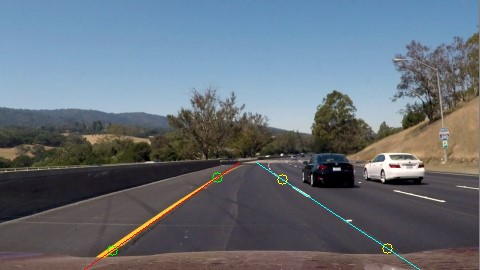
\includegraphics[width=\linewidth]{Figures/interpolation_lane_frame_0.jpg}
    \caption*{User input\\ frame 1}
\end{minipage}
\begin{minipage}[b]{0.45\linewidth}
    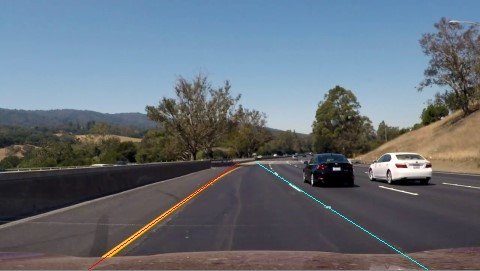
\includegraphics[width=\linewidth]{Figures/interpolation_lane_frame_10.jpg}
    \caption*{Interpolated lane placement\\ frame 10}
\end{minipage}
\vspace{5mm}\\
\begin{minipage}[b]{0.45\linewidth}
    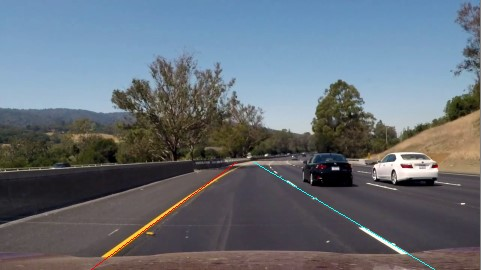
\includegraphics[width=\linewidth]{Figures/interpolation_lane_frame_20.jpg}
    \caption*{Interpolated lane placement\\ frame 20}
\end{minipage}
\begin{minipage}[b]{0.45\linewidth}
    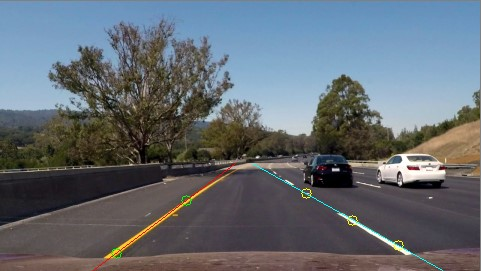
\includegraphics[width=\linewidth]{Figures/interpolation_lane_frame_30.jpg}
    \caption*{User input\\ frame 30}
\end{minipage}
\caption{Results from the interpolation method for lane tracking}
\label{fig:lane_tracking_interpolation}
\end{figure}


\subsubsection{Automatic Tracking}

Four different masking methods were tried, namely gray scale, RGB, HSV and HSL, in order to see which method gives the best results. The lane detection algorithm was tested on three different scenarios, NDS videos containing dashed lanes, see figure \ref{fig:dash_day}, NDS videos containing solid lanes, see figure \ref{fig:solid_day}, and NDS videos recorded during night time, see figure \ref{fig:night}. Three representative videos were used for each of the three scenarios and the results are presented below, in terms of percentage of detected lanes.

\begin{figure}[H]
    \centering    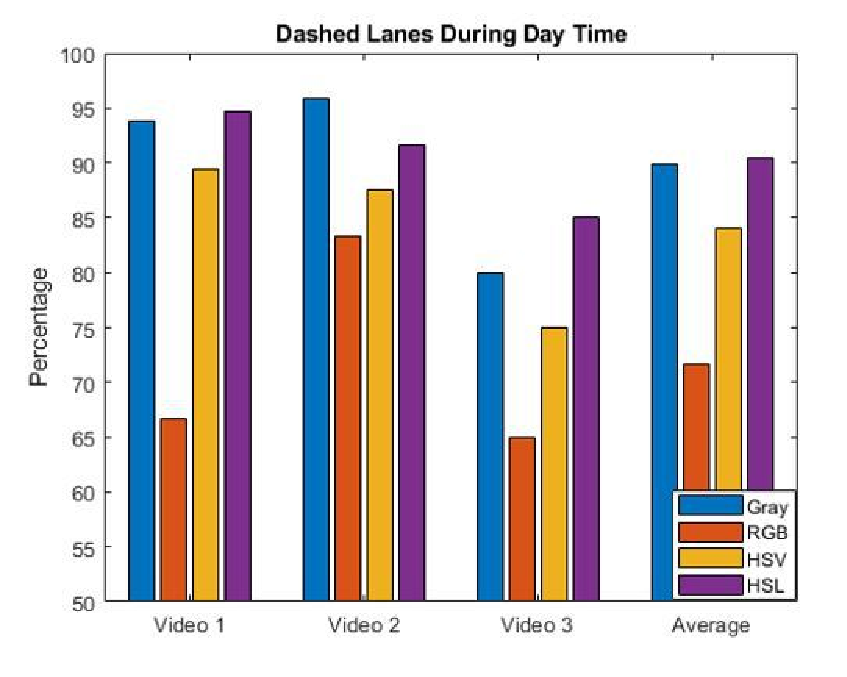
\includegraphics[width = 0.5\textwidth]{Figures/Result_01.pdf}
    \caption{Percentage of detected lanes for different masking methods on dashed lanes during day time}
    \label{fig:dash_day}
\end{figure}

\begin{figure}[H]
    \centering
    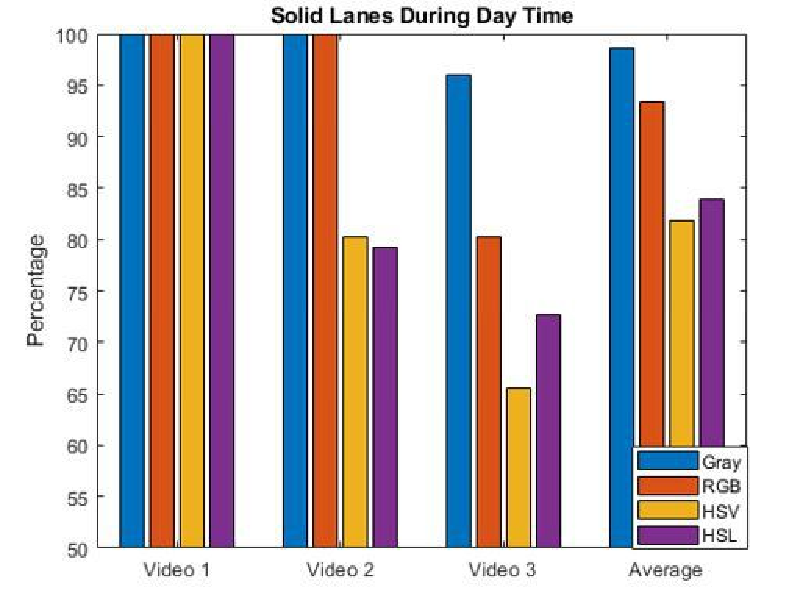
\includegraphics[width = 0.5\textwidth]{Figures/result_02.pdf}
    \caption{Percentage of detected lanes for different masking methods on continuous lanes during day time}
    \label{fig:solid_day}
\end{figure}

\begin{figure}[H]
    \centering
    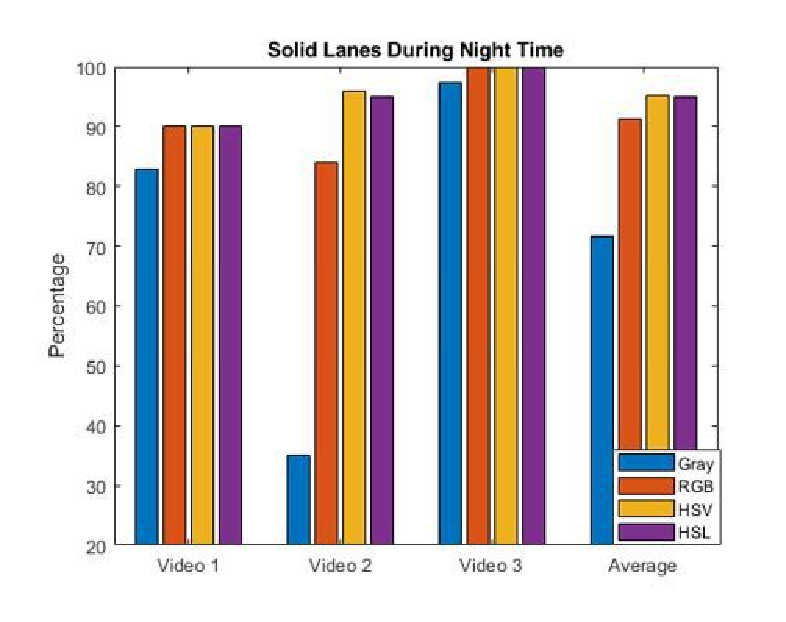
\includegraphics[width = 0.5\textwidth]{Figures/result_03.pdf}
    \caption{Percentage of detected lanes for different masking methods on continuous lanes during night time}
    \label{fig:night}
\end{figure}

Based on this experiment, gray scale seems to be overall best during videos recorded during day time. While HSV masking is more or less equal good as gray scale when it comes to videos recorded during night time.

\paragraph{Misdetection of lanes}
In order to determine how accurate the results presented in the previous section are, the percentage of misdetected lanes for each masking method was calculated. The ROI of the lane detection algorithm was defined in an area of the image where no lanes are present, and the percentage of misdetected lanes for each masking method was assessed. The experiment was done for videos recorded both during day time and videos recorded during night time. The results are presented in Table \ref{tab:misdetection}.


% \begin{figure}[H]
%     \centering
%     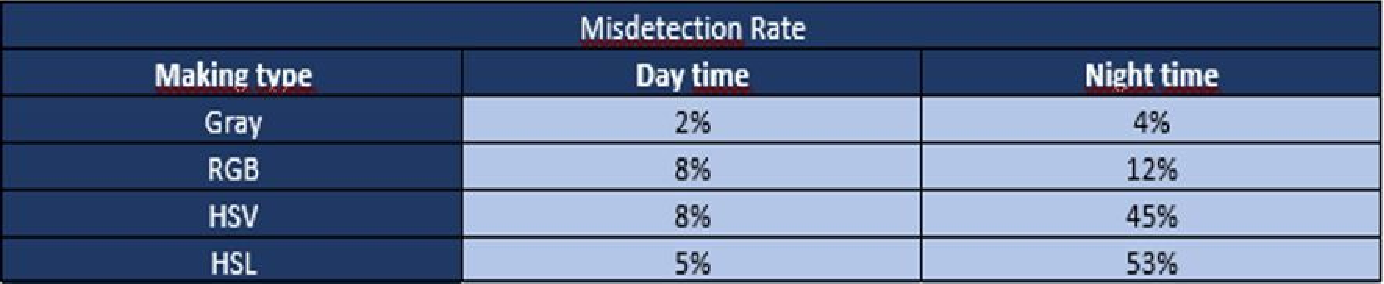
\includegraphics[width = 0.8\textwidth]{Figures/mis-detection.pdf}
%     \caption{Mis-detection of lanes for different masking methods during day and night time expressed in percentages}
%     \label{fig:misdetection}
% \end{figure}

\begin{table}[H]
    \centering
    \begin{tabular}{c|c|c}
         \multicolumn{3}{c}{\textbf{Mis-detectin Rate}} \\ \hline
         Making Type & Day Time $(\%)$ & Night Time $(\%)$ \\ \hline
         Gray & 2 & 4 \\
         RGB & 8 & 12 \\
         HSV & 8 & 45 \\
         HSL & 5 & 53
    \end{tabular}
    \caption{Mis-detection of lanes for different masking methods during day and night time expressed in percentages}
    \label{tab:misdetection}
\end{table}

The result shows that gray scale has by far the smallest percentage of misdetected lanes. The results also show that colour masking causes very high percentage of misdetected lanes during night time. A high misdetection rate leads to misleading result.

\paragraph{Flickering}

The result from the flickering test are present in figure \ref{fig:flick_day} and figure \ref{fig:flick_night}. The result in figure \ref{fig:flick_day} shows that automatic lane detection tends to have less flickering when analyse videos recorded during  day time compared to manual tracking of lanes. However, the result in figure \ref{fig:flick_night} shows that automatic lane detection tends to have more flickering when analyse videos recorded during night time compared to manual tracking of lanes.

\begin{figure}[H]
    \centering
    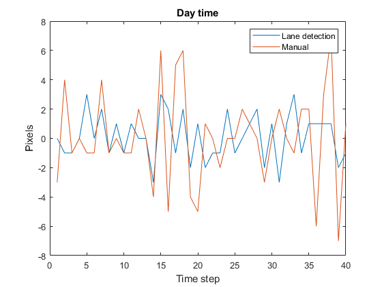
\includegraphics[width = 0.8\textwidth]{Figures/flick2.png}
    \caption{Flickering of the detected lanes during day time for manual tracking and automatic tracking of lanes}
    \label{fig:flick_day}
\end{figure}

\begin{figure}[H]
    \centering
    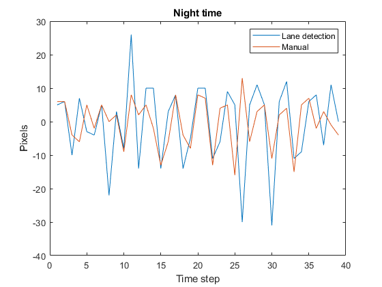
\includegraphics[width = 0.8\textwidth]{Figures/flick1.png}
    \caption{Flickering of the detected lanes during night time for manual tracking and automatic tracking of lanes}
    \label{fig:flick_night}
\end{figure}




\paragraph{Bird's eye transformation}
The figure below shows the perspective transform obtained on a test image. The end co-ordinates of the test image from the original view are selected as source and the destination co-ordinates(the co-ordinates of trapezoidal view as seen in figure of bird's eye transformation) are specified as a separate array. The source and destination on original and bird's view respectively are given as input to a transformation matrix. This is followed by a function named warped perspective in openCV library which modifies the translation,scaling and rotation matrix to give the resulting bird's eye view transformation as shown in the figure below.

\begin{figure}[H]
    \centering
    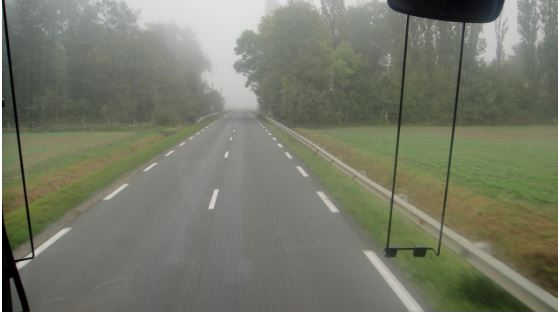
\includegraphics[width = 0.7\textwidth]{Figures/Originalview.JPG}
    \caption{Original view}
    \label{fig:my_label1}
\end{figure}
\begin{figure}[H]
    \centering
    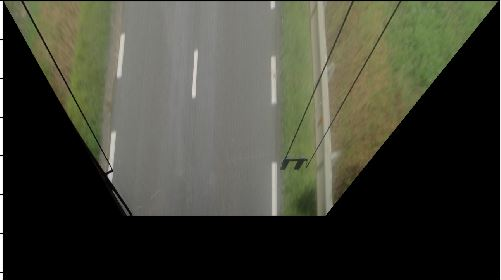
\includegraphics[width = 0.7\textwidth]{Figures/Bird'sview.JPG}
    \caption{Bird's eye transformation}
    \label{fig:my_label2}
\end{figure}
\subsection{Heading Angle}
Only the triangulation method was implemented for the heading angle. Even though this method relied on the user to define the POV wheel placement on the ground, it proved to be the easiest to implement and provided good results, as presented below.

% \subsubsection{Method 1 for Heading Angle: Triangulation}

Figure clearly shows how the POV is maneuvering: first by having a small heading angle which increases to reach a maximum during the maneuver and then decreases back to a low value when the POV is ending the maneuver to continue straight ahead. 

In Figure \ref{fig:heading_angle} and the graphs that follow, "Event 1" refers to the annotation of an event where the SV is changing lanes, while "Event 2" refers to the annotation of an event where the SV stays in its lane (i.e not changing the yaw angle of the camera). It is seen in Figure \ref{fig:heading_angle} that Event 1 seems to have a jumpy behaviour and that is because the SV is changing lanes at the same time as the POV is changing lanes, and because the event takes place on a curved road. Those added to the assumption errors and hence show a more jerky motion of the POV's heading angle.


\begin{figure}[H]
\centering
\begin{minipage}[b]{0.49\textwidth}
    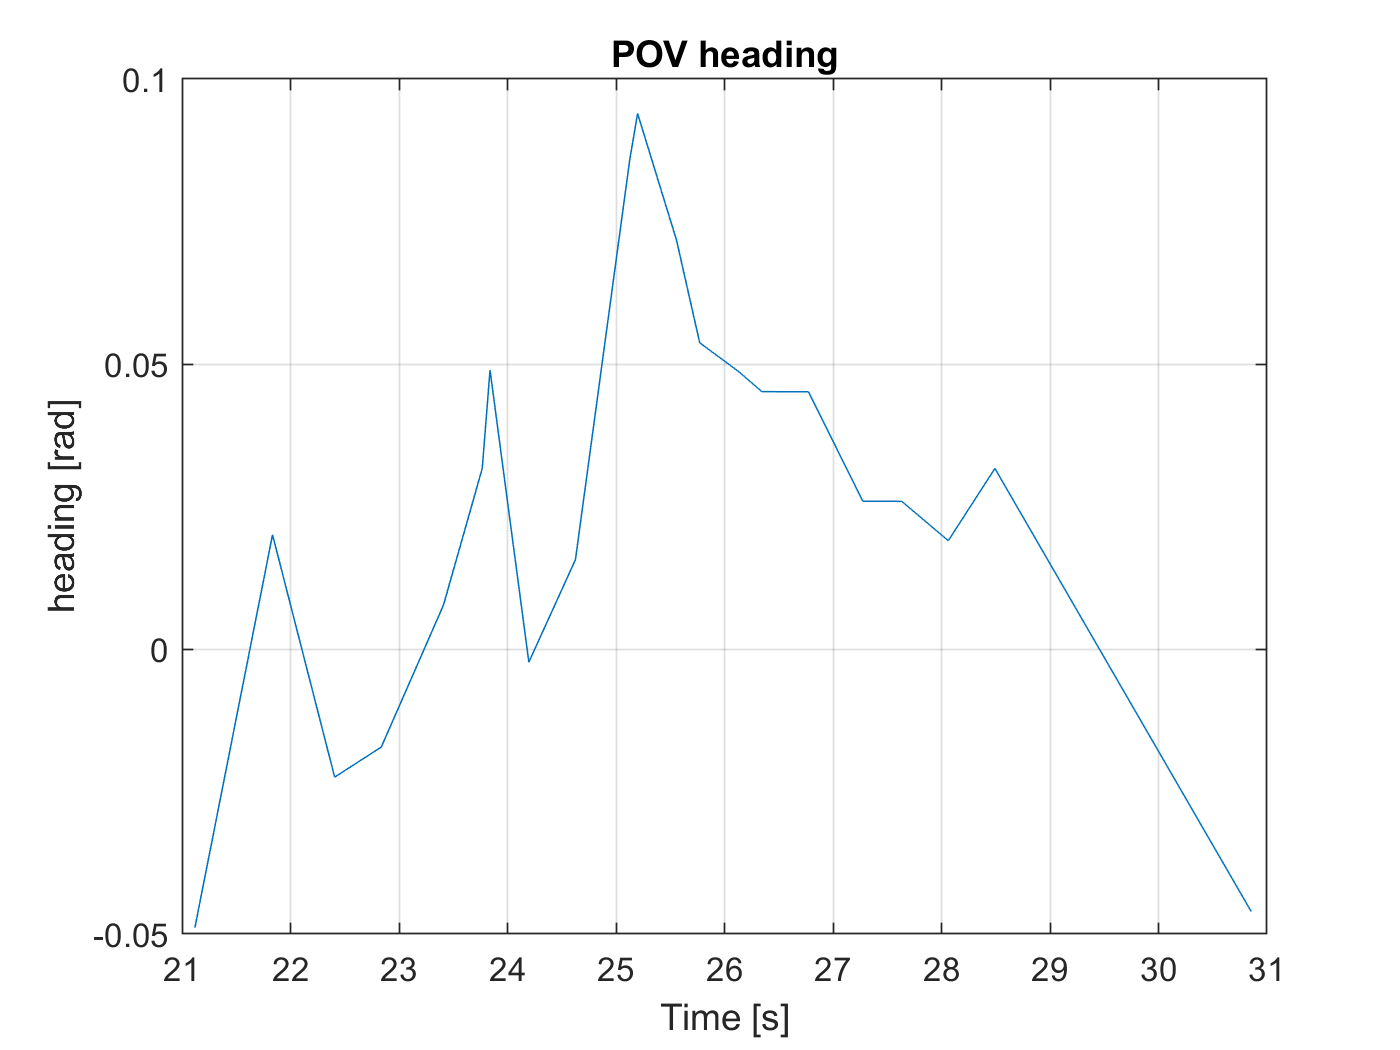
\includegraphics[width=\textwidth]{FiguresMat/pov_heading_10794257.png}
    \caption*{Event 1}
\end{minipage}
\begin{minipage}[b]{0.5\textwidth}
    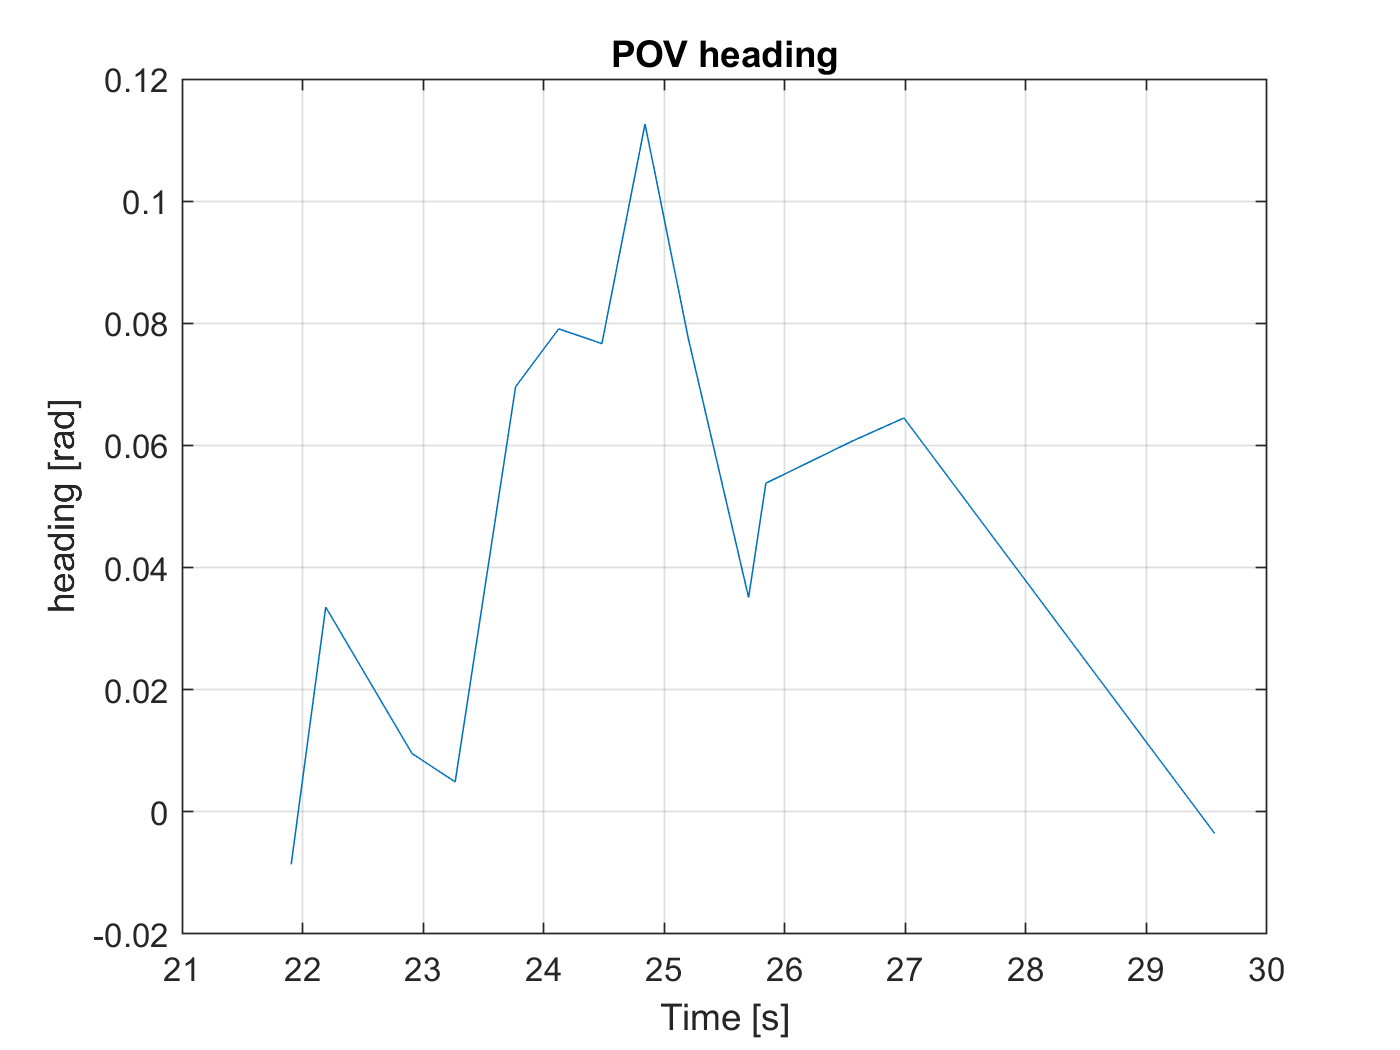
\includegraphics[width=\textwidth]{FiguresMat/pov_heading_116147345.png}
    \caption*{Event 2}
\end{minipage}
\caption{POV Heading Angle}
\label{fig:heading_angle}
\end{figure}

\subsection{Lateral Offset}

The plots presented blow were done for critical lane-changing events in the SHRP2 data that have radar range available. These were the same as "Event 1" and "Event 2" presented earlier.  

\subsubsection{Filtering}

The acquired lateral offset from the annotation tool was used to calculate the lateral offset rate to the POV. It was found that the raw output was not smooth enough and required filtering to gain reasonable lateral offset rate values, as shown in Figures \ref{fig:lat_offset_event1} and \ref{fig:lat_offset_event2}. Better results were acquired after applying two filters to the estimated range before calculating the range rate. Filter specifications are presented below in Table \ref{tab:filters}.

\begin{table}[H]
    \centering
\begin{tabular}{l|l|l}
    \textbf{Name} & \textbf{Type} & \textbf{Specification} \\
    \hline
    filter 1&  Savago & Poly order 2 and window length 11\\
    filter 2& Moving Average & Window length 11 frames
\end{tabular}
    \caption{Filters used on the raw estimated range}
    \label{tab:filters}
\end{table}


\begin{figure}[H]
    \centering
    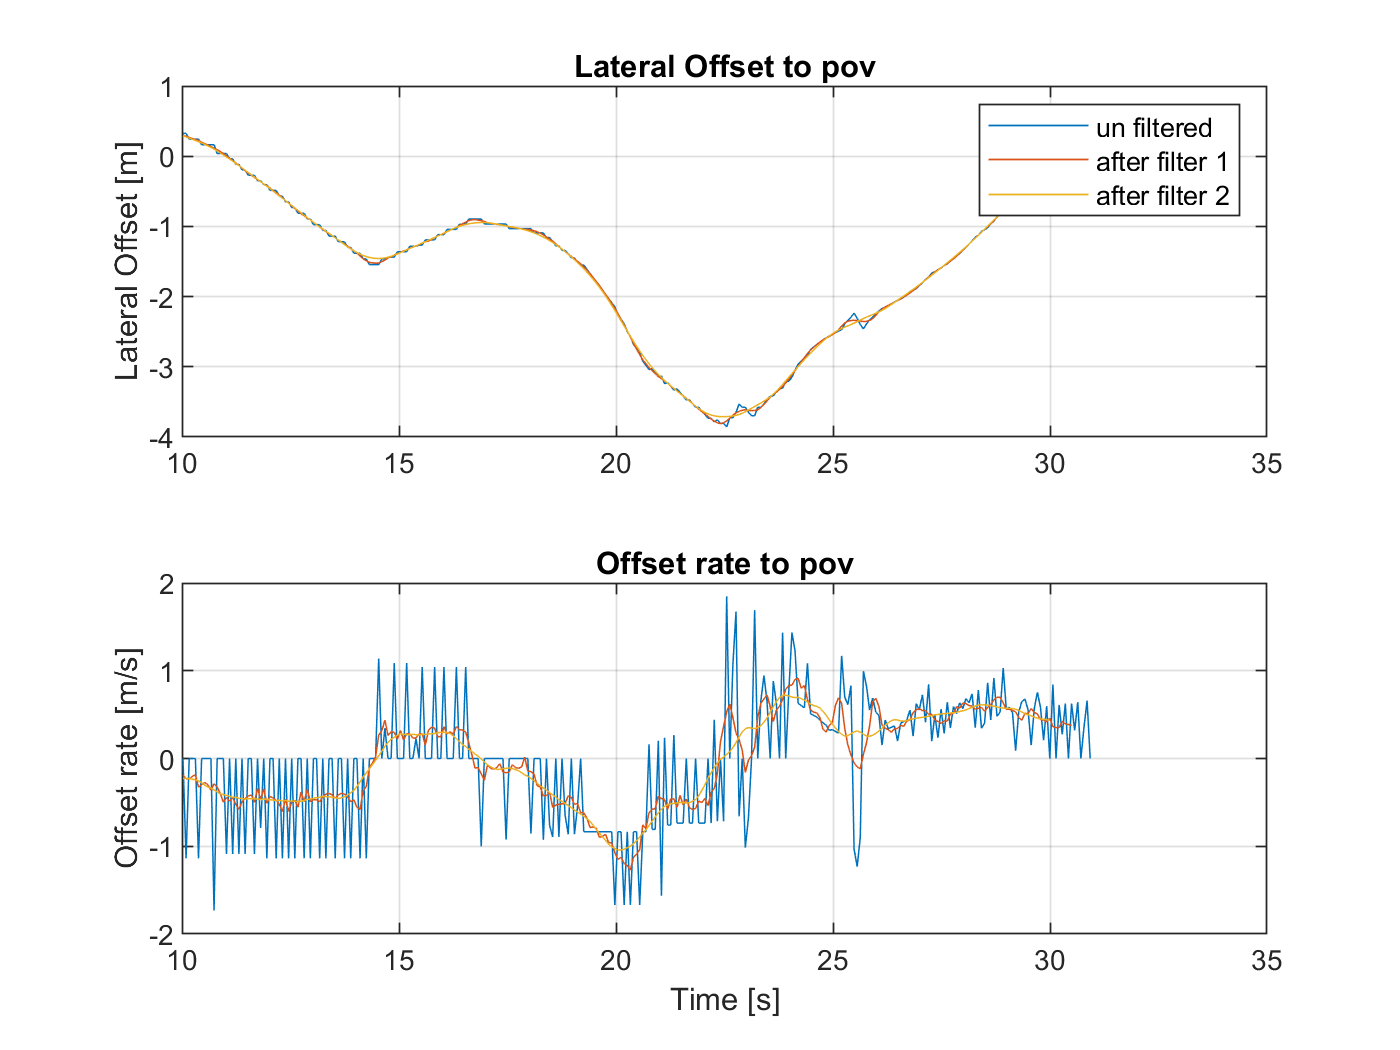
\includegraphics[width=0.8\textwidth]{FiguresMat/filter_compare_lateral_10794257.png}
    \caption{Estimated Lateral offset and offset rate for Event 1}
    \label{fig:lat_offset_event1}
\end{figure}

\begin{figure}[H]
    \centering
    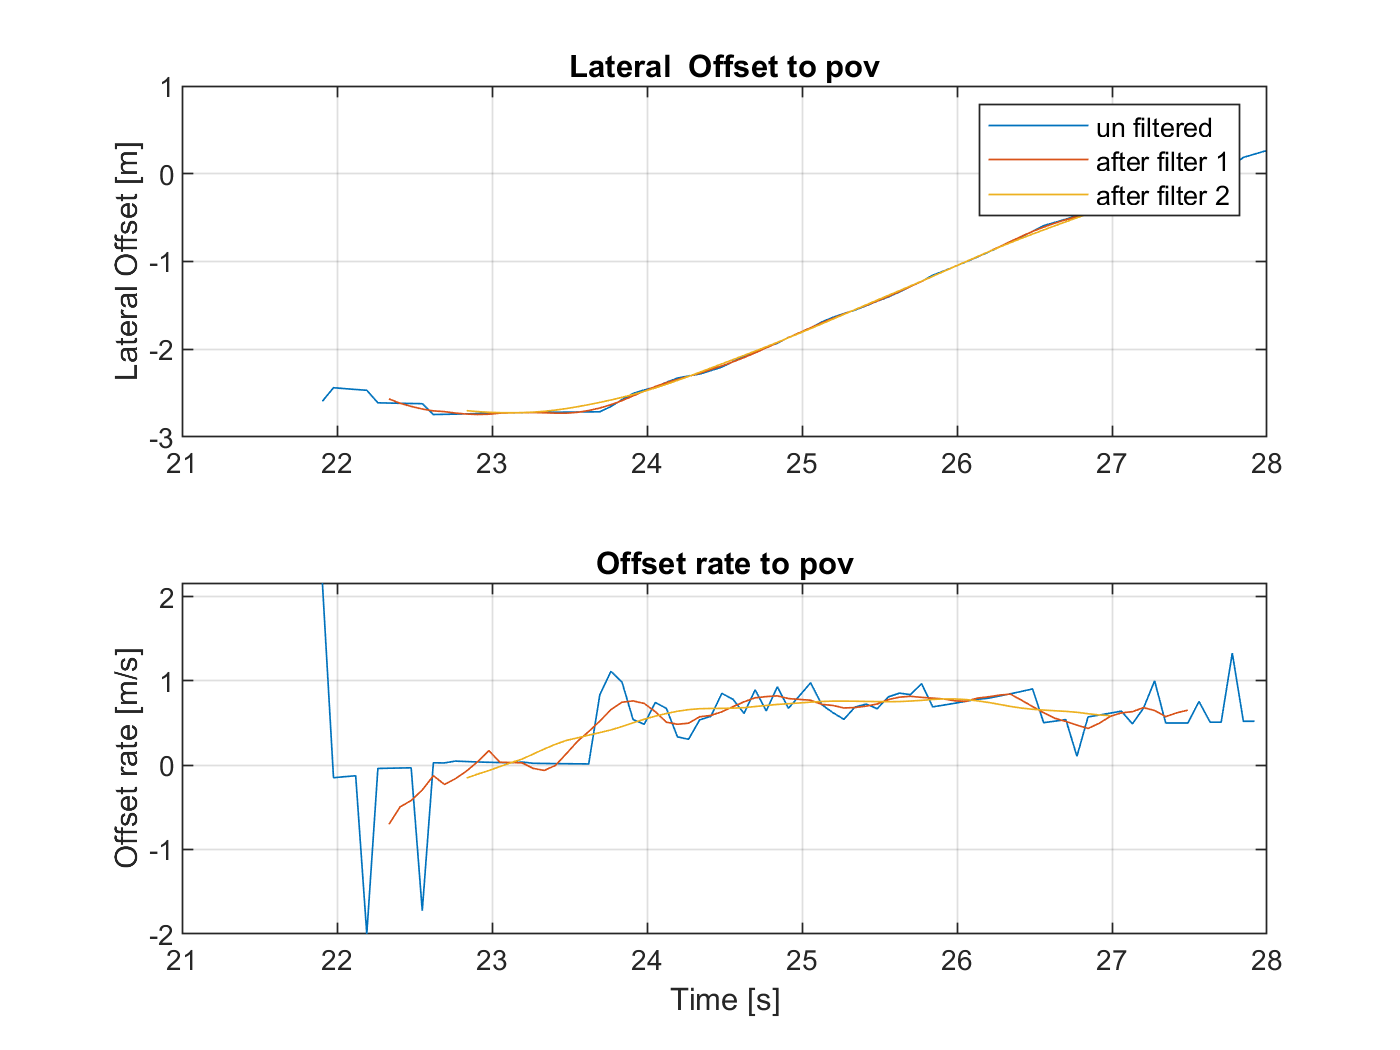
\includegraphics[width=0.8\textwidth]{FiguresMat/filter_compare_lateral_116147345.png}
    \caption{Estimated Lateral offset and offset rate for Event 2}
    \label{fig:lat_offset_event2}
\end{figure}


\subsubsection{Comparing Estimated Lateral Offset to Radar Data}

After filtering, the results of the pixel width method were compared to the available radar data, as shown in Figures \ref{fig:lat_offset_vs_radar_event1} and \ref{fig:lat_offset_vs_radar_event2}. As seen in these figures, the lateral offset gained from the pixel width method followed approximately the same shape as that of the radar data in both events 1 and 2. 

In event 1 of Figure \ref{fig:lat_offset_vs_radar_event1}, it is apparent how the SV was in the same lane as the POV, as the lateral offset was $\approx 0[m]$. The SV changed lane after $\approx 22[s]$, then the POV cut in-front of the SV until the POV was completely in the same lane, as the lateral offset returned to $\approx 0[m]$. 

\begin{figure}[H]
    \centering
    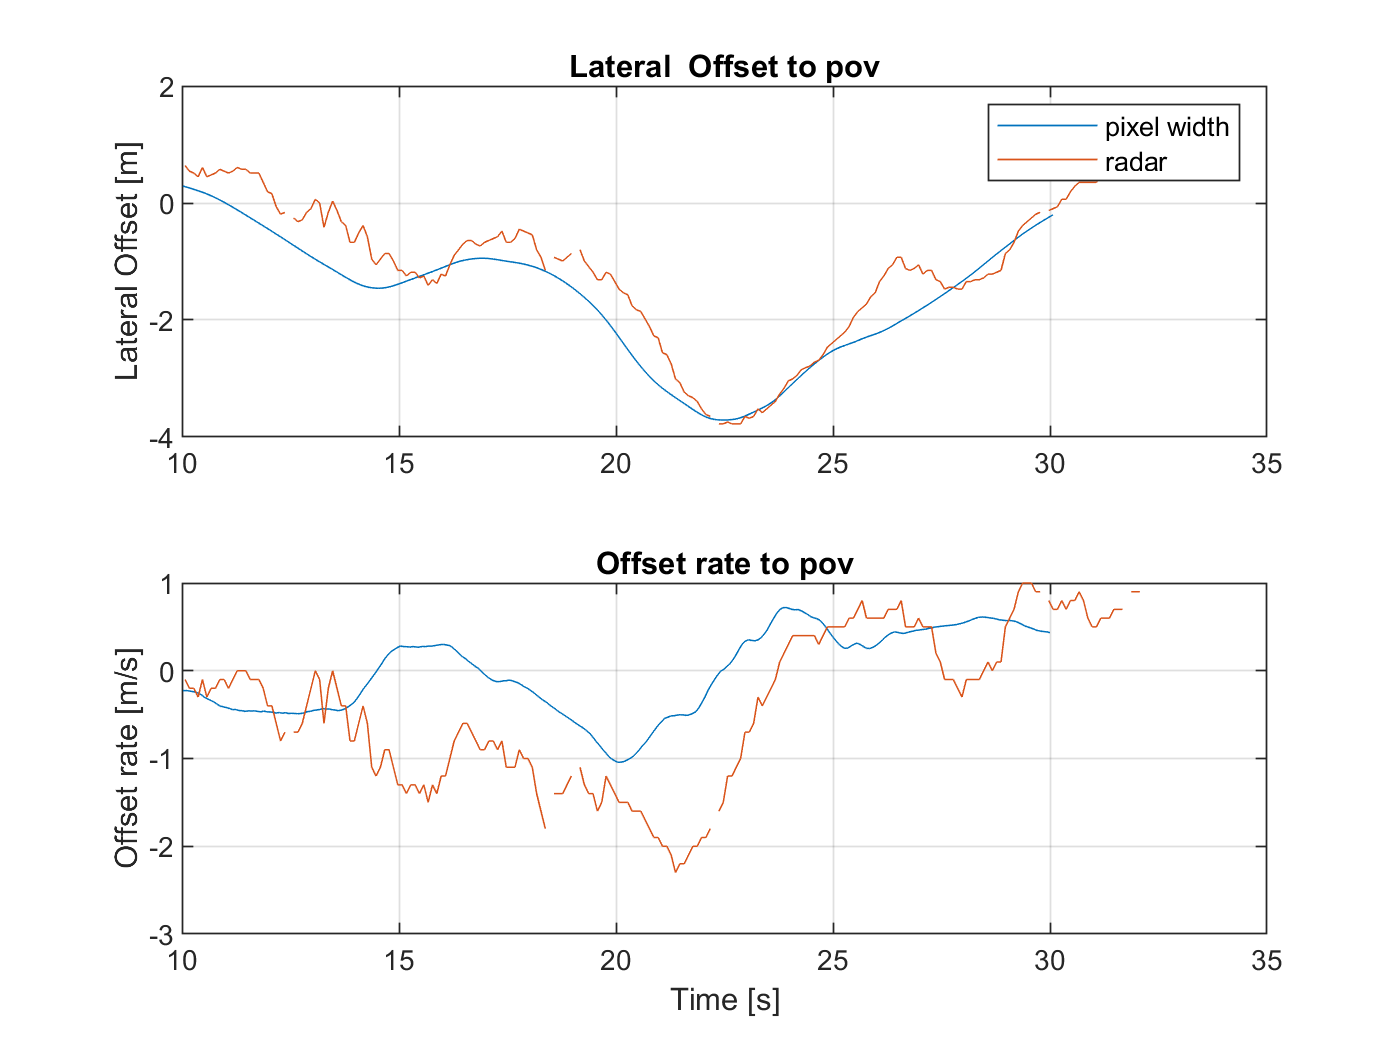
\includegraphics[width=0.8\textwidth]{FiguresMat/radar_compare_lateral_10794257.png}
    \caption{Estimated Lateral Offset vs Radar Data Event 1}
    \label{fig:lat_offset_vs_radar_event1}
\end{figure}

In event 2 of Figure \ref{fig:lat_offset_event2}, it is apparent how the SV was already in a different lane from the POV before the critical event, as the lateral offset was $\approx -3[m]$. After $\approx 24[s]$, the POV started to cut in-front of the SV until the POV is completely in the same lane as the SV, as the lateral offset returned to $\approx 0[m]$

\begin{figure}[H]
    \centering
    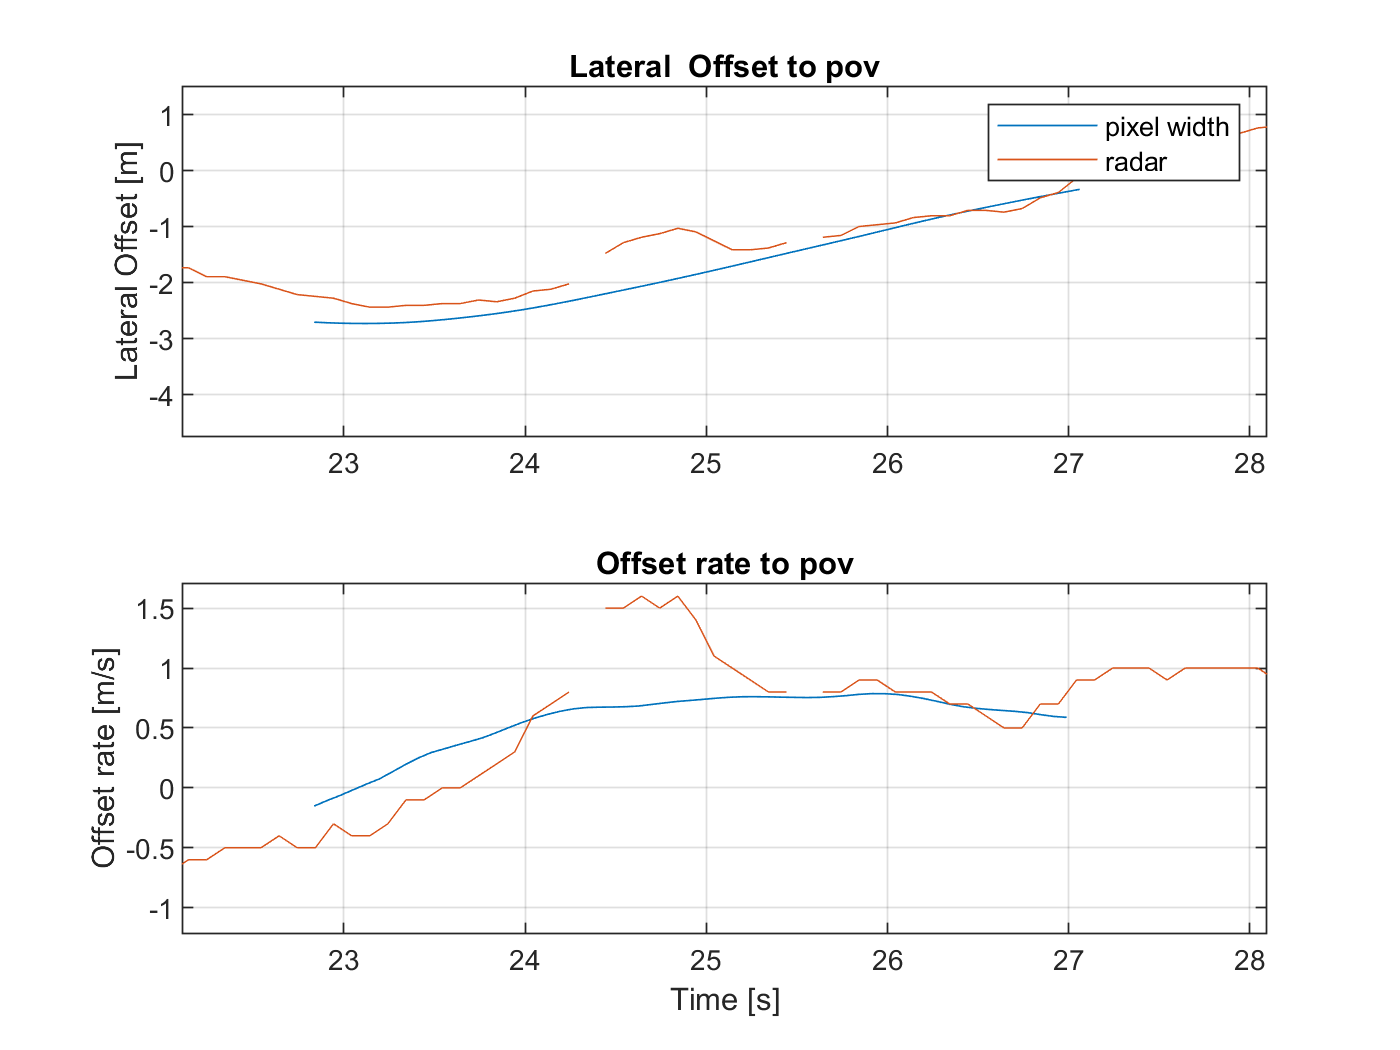
\includegraphics[width=0.8\textwidth]{FiguresMat/radar_compare_lateral_116147345.png}
    \caption{Estimated Lateral Offset vs Radar Data Event 2}
    \label{fig:lat_offset_vs_radar_event2}
\end{figure}

The lateral offset rate, however,  did deviate more from the radar data, but did so more in event 1, where the SV was changing lane before the critical event, compared to event 2, where the SV was in the same lane for the entire duration of the critical event.




% \subsubsection{Method 1 for Lateral Offset}

\subsubsection{Comparing Triangulation method to Pixel Width method and Radar Data}
The results found above were compared to the estimated offset gained from the triangulation method, as presented in Figure \ref{fig:triangulation_comparison_latoffset}. As seen in this figure, the lateral offset using this method in event 1 deviates more from the both radar and the estimated offset gained from the pixel width method. For event 2, however, both methods produce approximately the same results. Due to time constraints, lateral offset rate gained from the triangulation method was not compared to the other results. 

\begin{figure}[H]
    \centering
\begin{minipage}[b]{0.49\textwidth}
    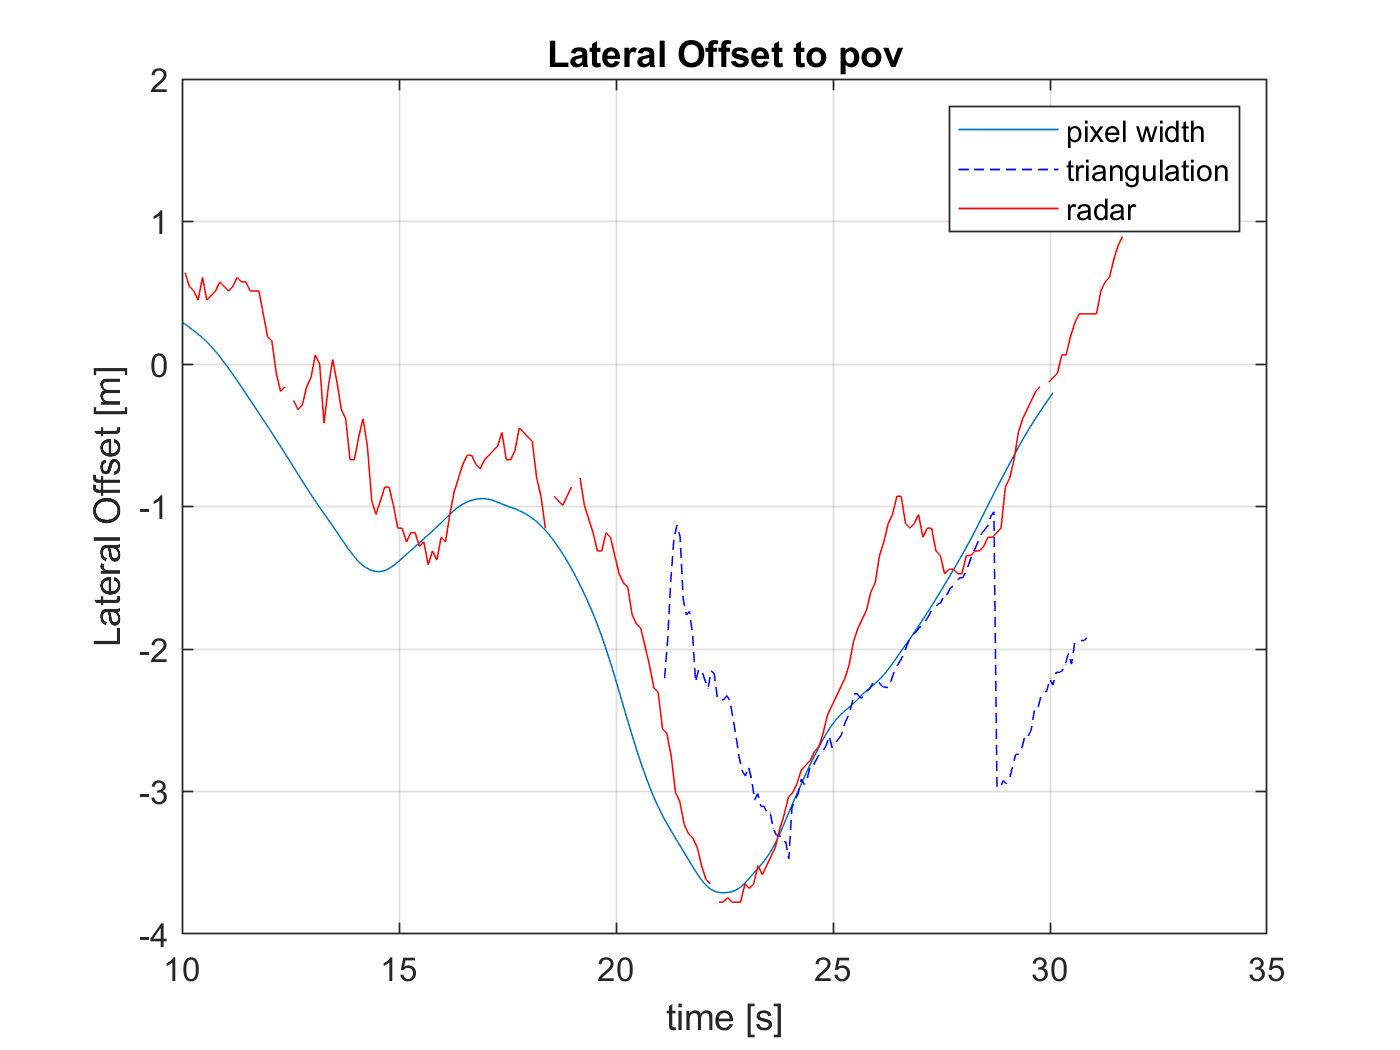
\includegraphics[width=\textwidth]{FiguresMat/homography_comparison_lat_10794257.png}
    \caption*{Event 1}
\end{minipage}
\begin{minipage}[b]{0.50\textwidth}
    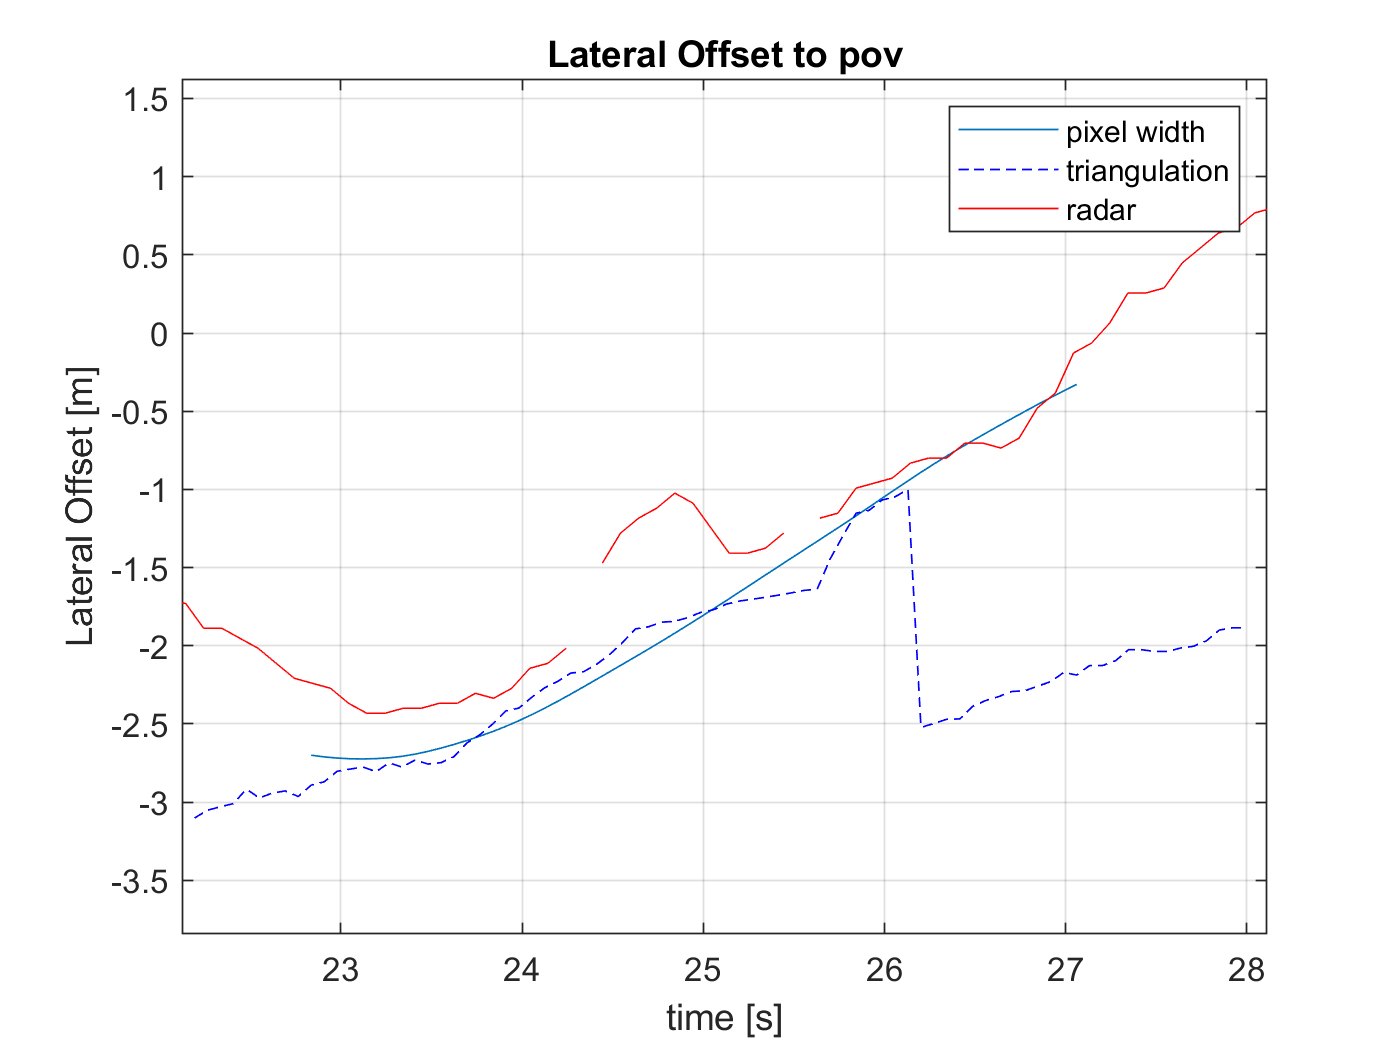
\includegraphics[width=\textwidth]{FiguresMat/homography_comparison_lat_116147345.png}
    \caption*{Event 2}
\end{minipage}
\caption{Comparing the two methods with Radar Data}
\label{fig:triangulation_comparison_latoffset}
\end{figure}

Please note that there is something wrong with the sign conversion when plotting the triangulation method in Figure \ref{fig:triangulation_comparison_latoffset}, that's why the lateral offset does the sudden jump after 26[s]. The same problem shows up in Figures \ref{fig:lat_offset_error_distance} and \ref{fig:lat_offset_error_heading}. This issue has been fixed in the tool but at the time of writing of the report (\today), the team does not have access to the updated figures. The report will be updated once the figures are acquired after the holidays.

\subsubsection{Estimation Error}

Using the radar data as reference, the error for different lateral offsets was calculated, as shown in Figure \ref{fig:lat_offset_error_distance} where it is apparent how the pixel width method remains within an error in the range $\in(-0.5, 1.5)[m]$ in event 1. In event 2, the error value is smaller, but remains within the same range. It is also apparent that the lateral offset error using the pixel width method is not affected by the actual lateral offset. On the other hand, the triangulation method shows more fluctuation when it comes to calculating the lateral offset to POV. However, this method, as discussed earlier, allows for the calculation of the lateral offset to the lane lines, and not just the relative offset between the two vehicles.

\begin{figure}[H]
\begin{minipage}[b]{0.49\textwidth}
    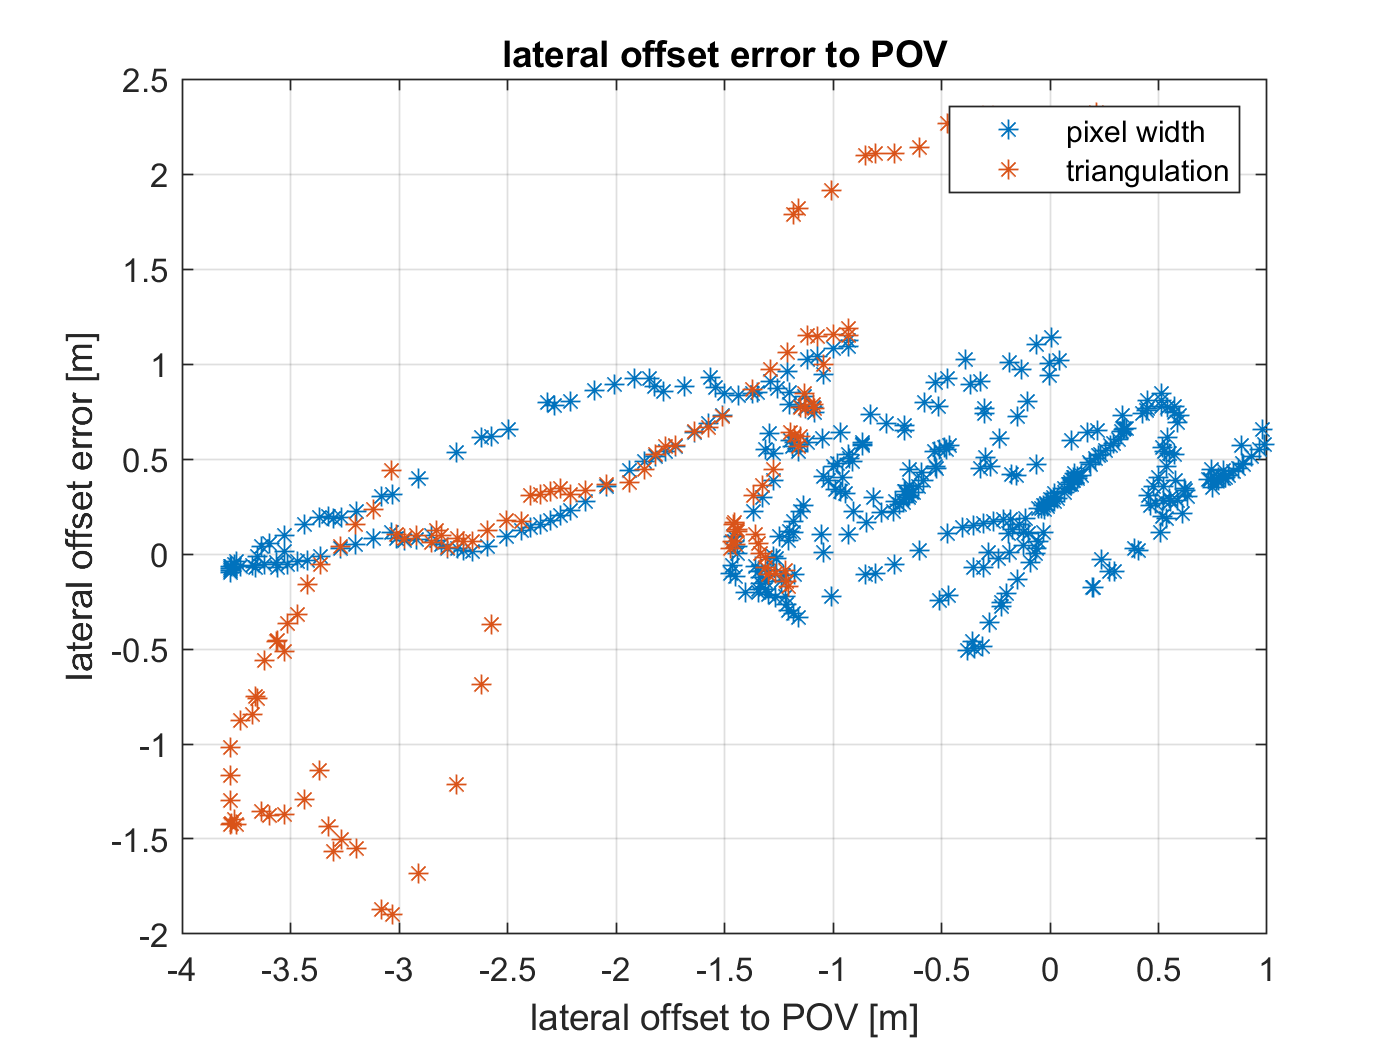
\includegraphics[width=\textwidth]{FiguresMat/range_error_lat_10794257.png}
    \caption*{Event 1}
\end{minipage}
\begin{minipage}[b]{0.50\textwidth}
    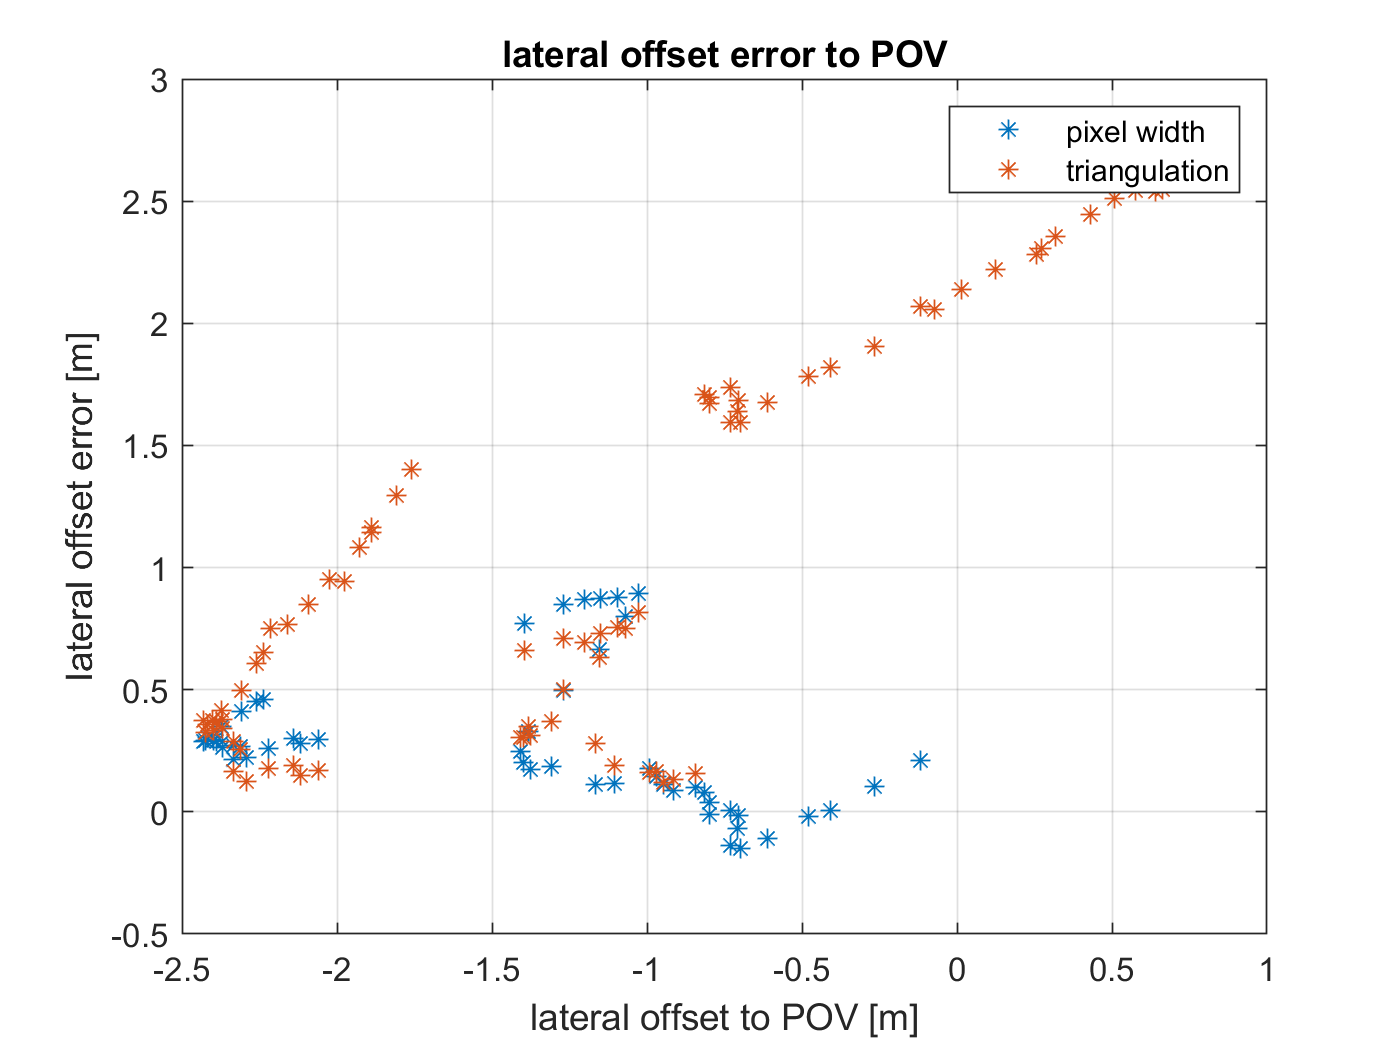
\includegraphics[width=\textwidth]{FiguresMat/range_error_lat_116147345.png}
    \caption*{Event 2}
\end{minipage}
\caption{POV lateral offset error vs POV actual lateral offset}
\label{fig:lat_offset_error_distance}
\end{figure}

This was also calculated for different heading angles, as shown in Figure \ref{fig:lat_offset_error_heading} which shows the relation between the POV's heading angle and the lateral offset estimation. From those plots, there doesn't seem to be a solid relation between the heading angle and the error in estimating the lateral offset with the pixel width method. The error seems to mostly stay in the range $\in(-0.5, 1)[m]$. The triangulation method shows a larger offset error compared to the pixel width method. Since the figure only shows two events, the results of this test are deemed to be inconclusive.

\begin{figure}[H]
\centering
\begin{minipage}[b]{0.49\textwidth}
    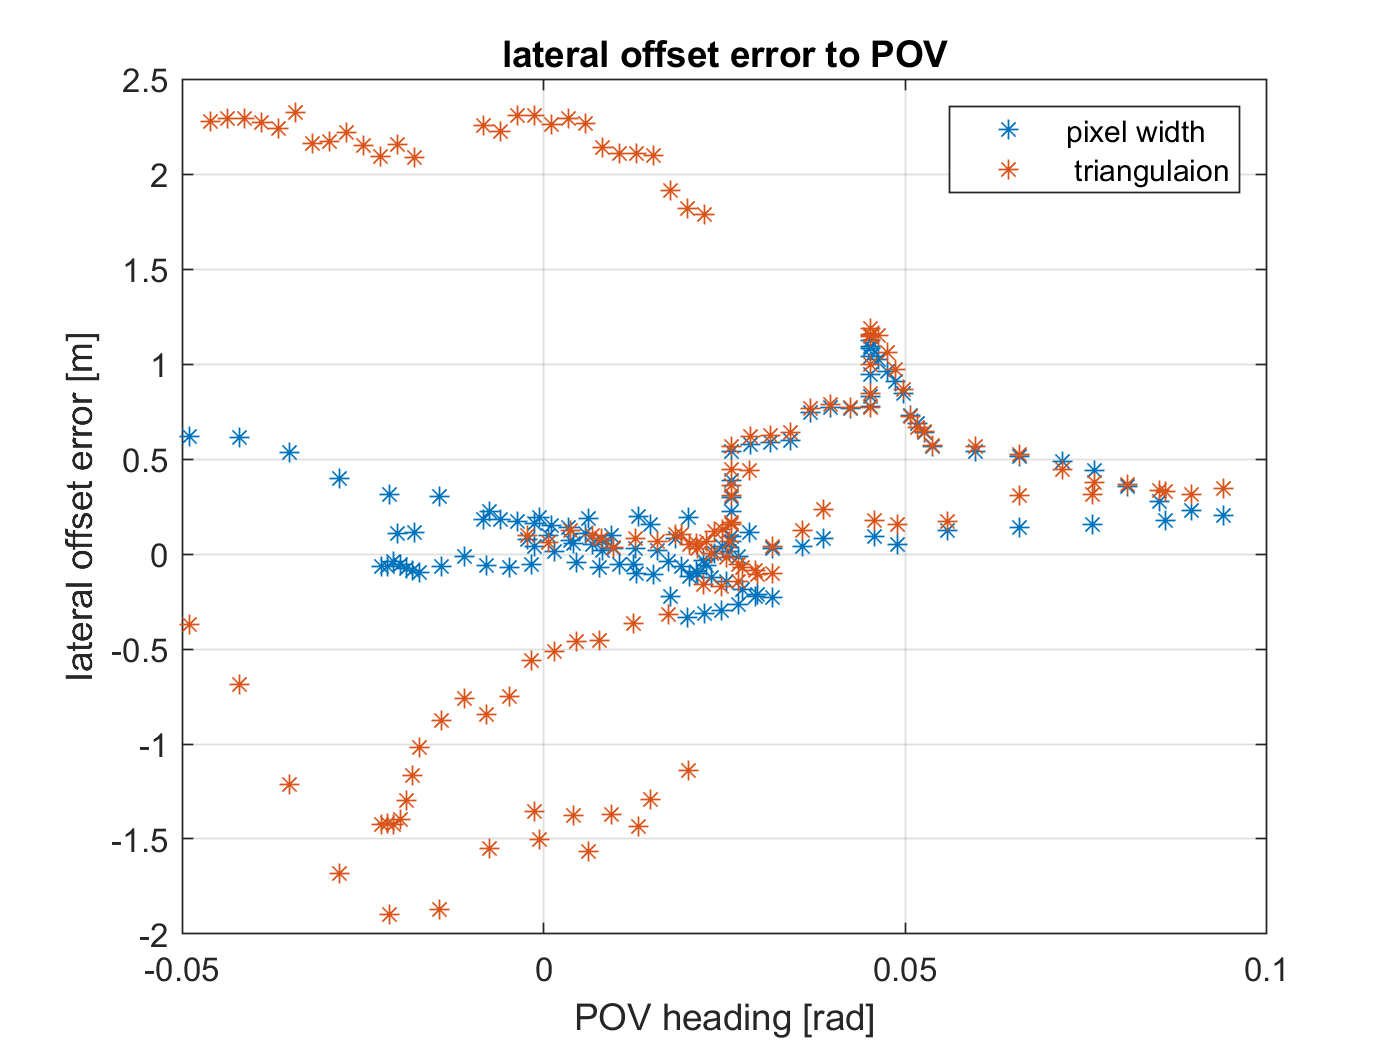
\includegraphics[width=\textwidth]{FiguresMat/range_heading_error_lat_10794257.png}
    \caption*{Event 1}
\end{minipage}
\begin{minipage}[b]{0.5\textwidth}
    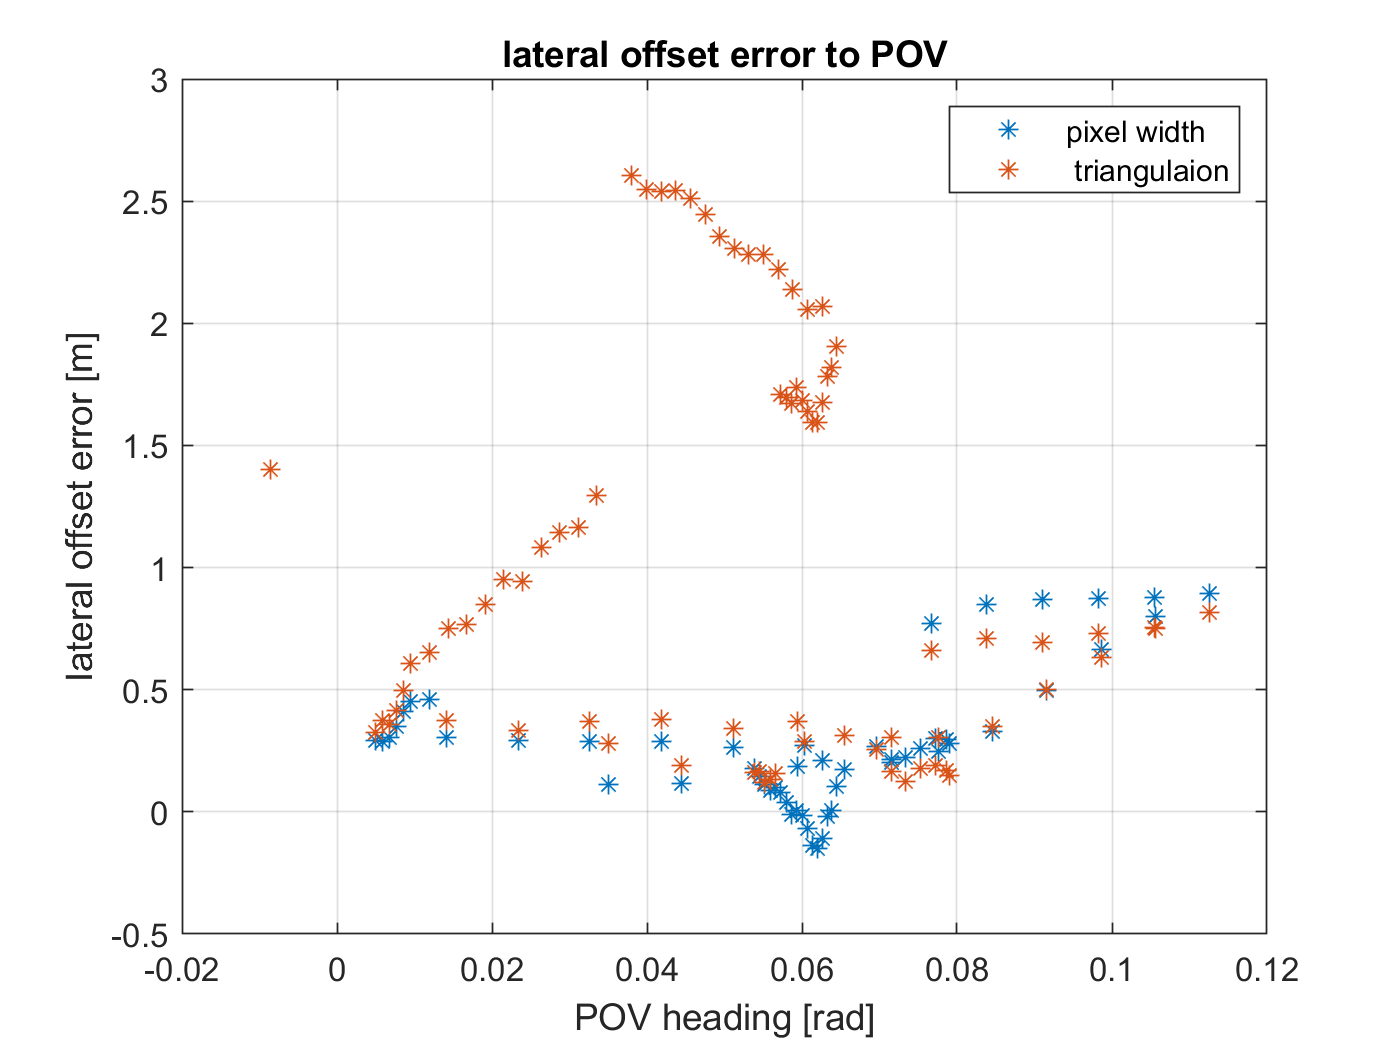
\includegraphics[width=\textwidth]{FiguresMat/range_heading_error_lat_116147345.png}
    \caption*{Event 2}
\end{minipage}
\caption{POV lat offset error vs POV estimated heading angle}
\label{fig:lat_offset_error_heading}
\end{figure}

\subsection{Range estimation}
The plots presented blow were done for critical lane-changing events in the SHRP2 data that have radar range available. These were the same as "Event 1" and "Event 2" presented earlier.  

% \subsubsection{Method 1 for Range Estimation: Pixel width}
\subsubsection{Filtering}
The estimated range acquired from the annotation tool was used to calculate the range rate to the POV. As was the case for the lateral offset, the estimated range had to be filtered to gain reasonable range rate values, as shown in Figures  \ref{fig:range_filtering_event1} and \ref{fig:range_filtering_event2}. This was done in the same was as for the lateral offset with the same filter specifications presented in Table \ref{tab:filters}.


\begin{figure}[H]
    \centering
    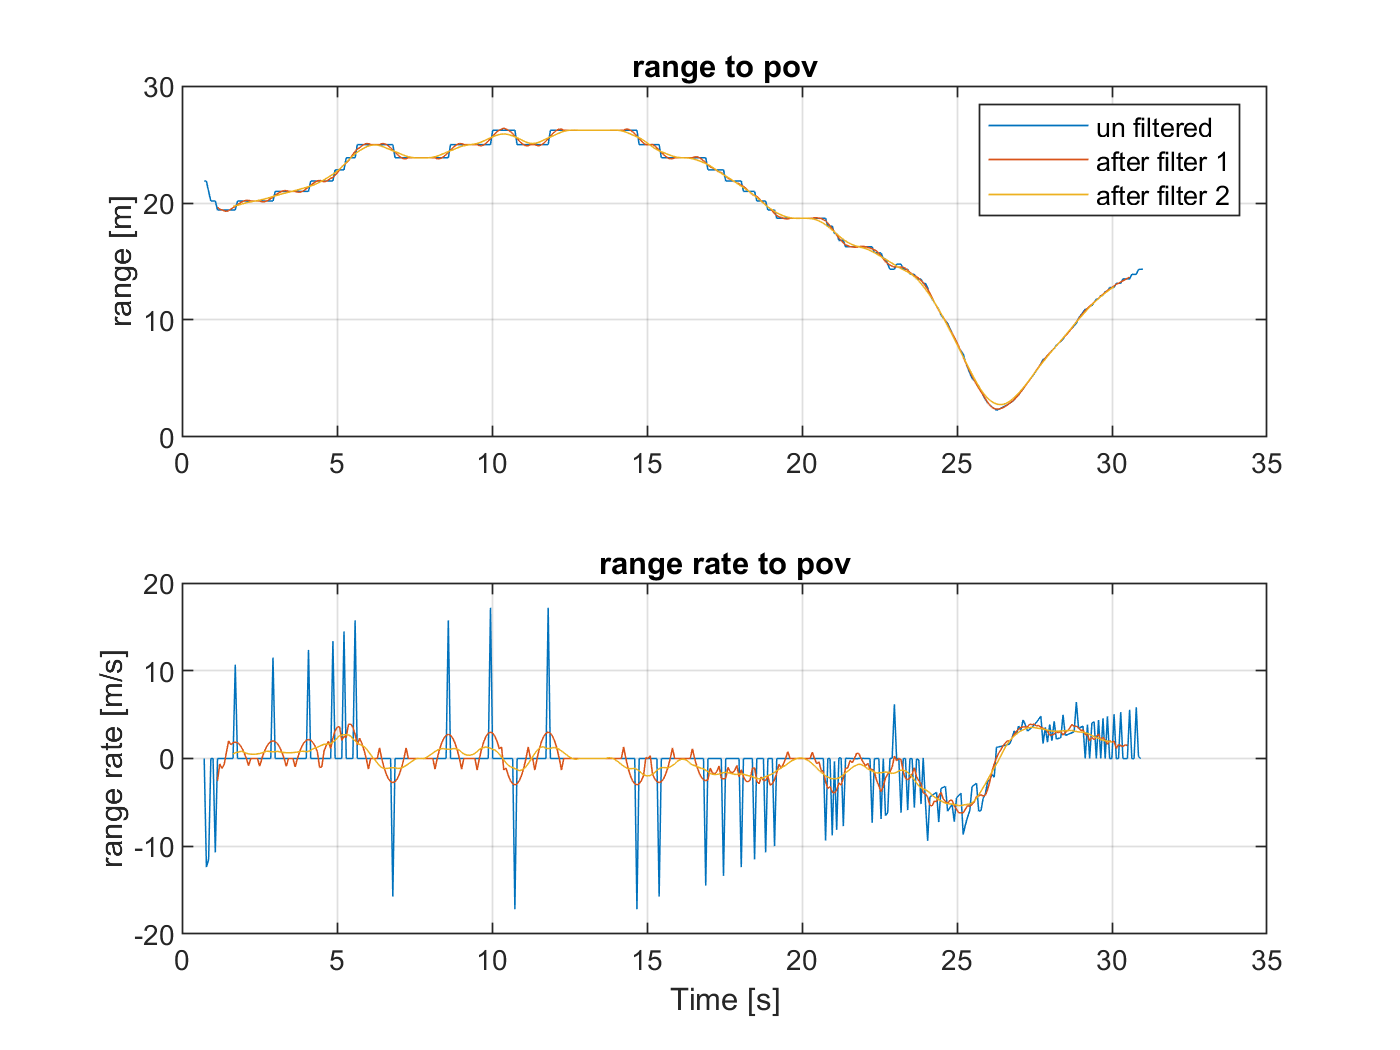
\includegraphics[width=0.8\textwidth]{FiguresMat/filter_compare_10794257.png}
    \caption{Range and Range rate with filtering Event 1}
    \label{fig:range_filtering_event1}
\end{figure}

\begin{figure}[H]
    \centering
    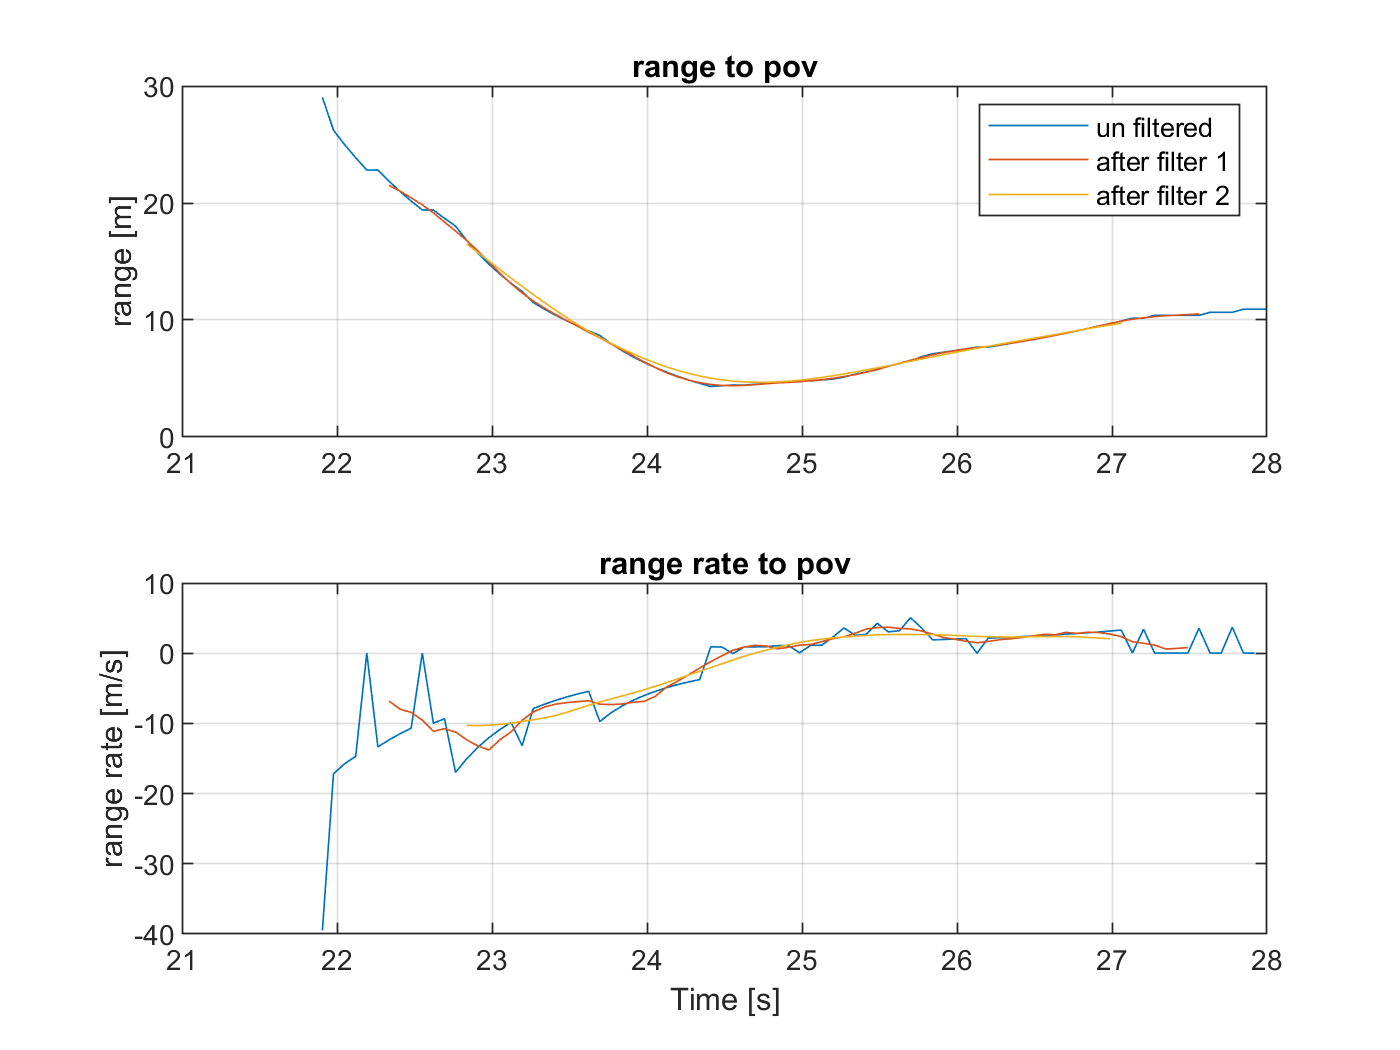
\includegraphics[width=0.8\textwidth]{FiguresMat/filter_compare_116147345.png}
    \caption{Range and Range rate with filtering Event 2}
    \label{fig:range_filtering_event2}
\end{figure}

\subsubsection{Comparing Estimated Range to Radar Data}
After filtering, the range and range rate attained from the pixel width method were compared to the radar, as shown in Figures \ref{fig:range_vs_radar_event1} and \ref{fig:range_vs_radar_event2}. From these figures, it appeared that the relative speed between the SV and the POV was higher in event 2 of Figure \ref{fig:range_vs_radar_event1} compared to event 1 of Figure \ref{fig:range_vs_radar_event2}. 

In both cases, the estimated range captured the same shape as that of the radar data. However, there appeared to be a constant offset in the range estimation in both cases, which meant that the POV seemed further away that it actually was.

\begin{figure}[H]
    \centering
    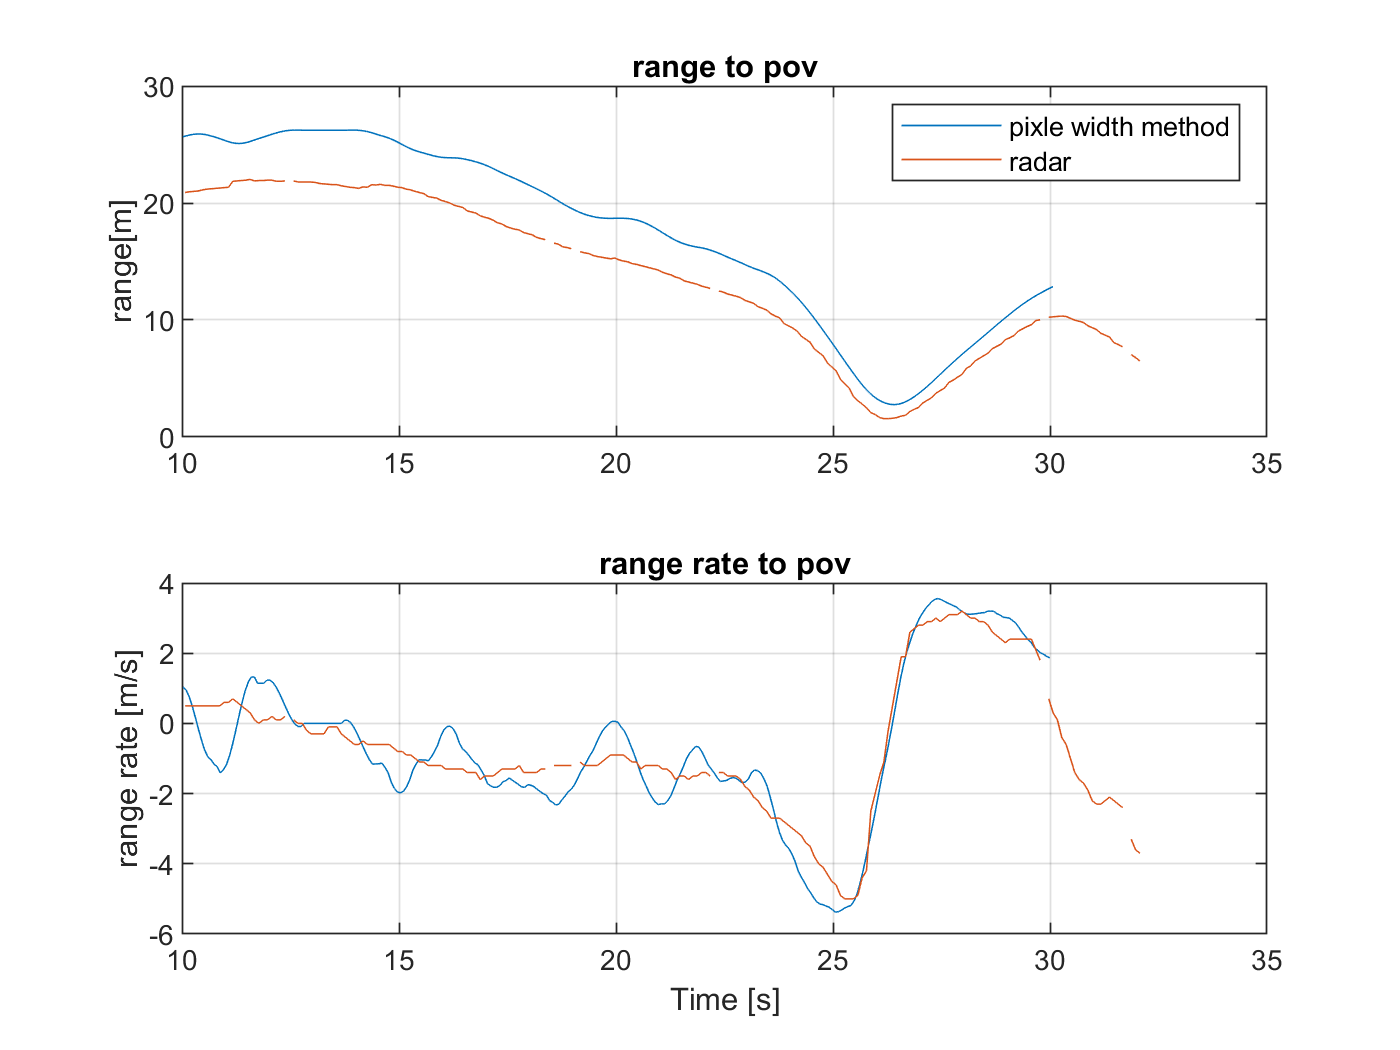
\includegraphics[width=0.8\textwidth]{FiguresMat/radar_compare_10794257.png}
    \caption{Estimated Range vs Radar Data Event 1}
    \label{fig:range_vs_radar_event1}
\end{figure}

\begin{figure}[H]
    \centering
    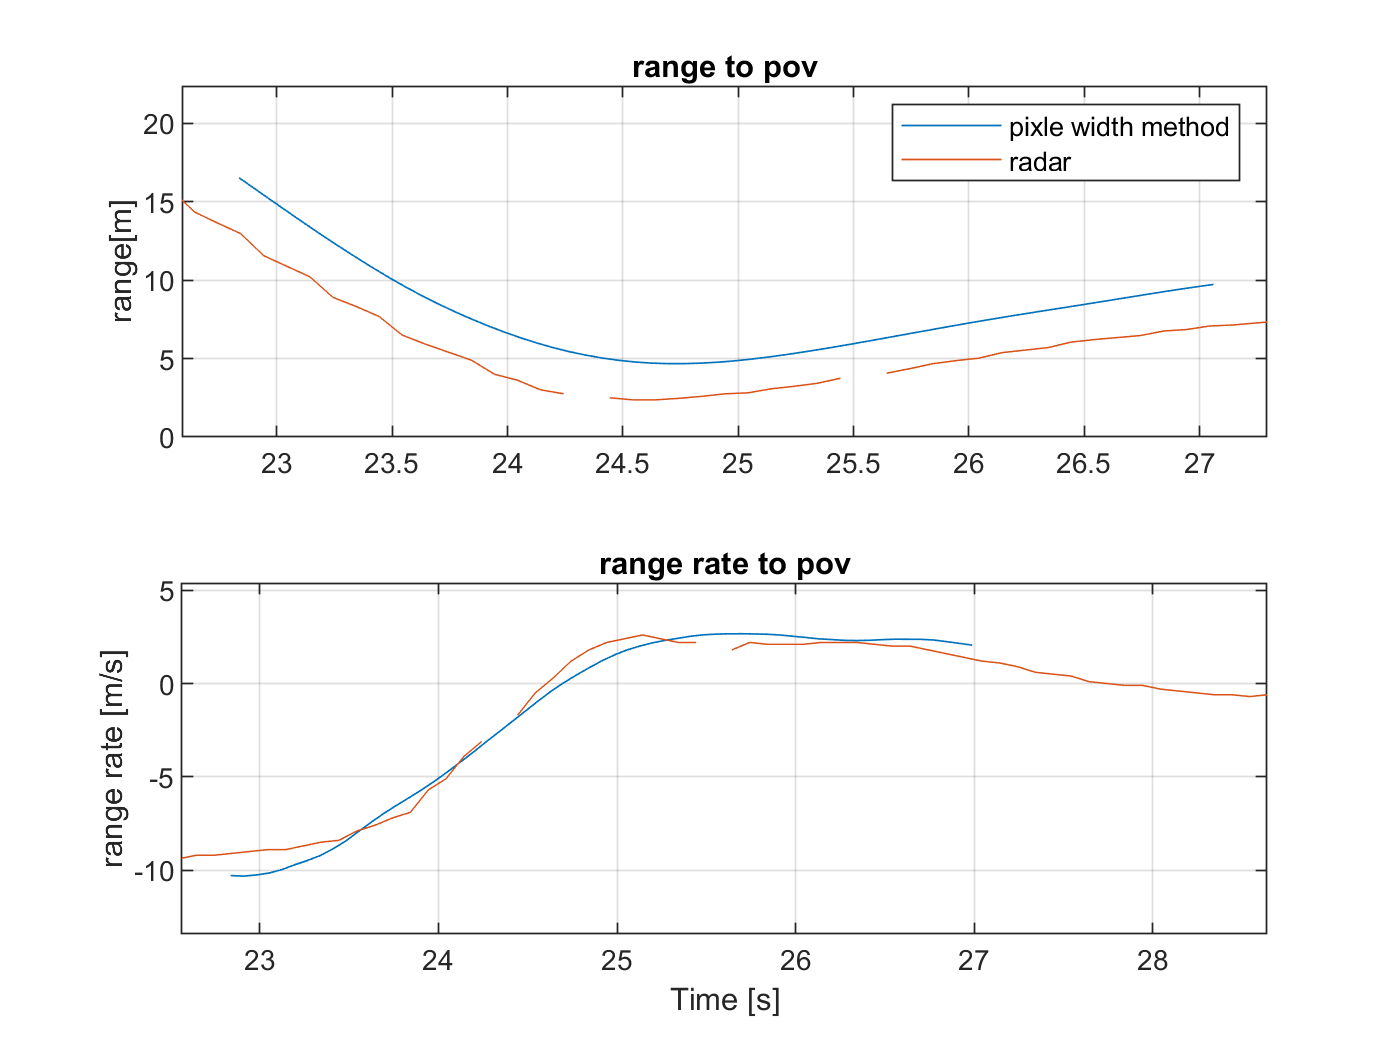
\includegraphics[width=0.8\textwidth]{FiguresMat/radar_compare_116147345.png}
    \caption{Estimated Range vs Radar Data Event 2}
    \label{fig:range_vs_radar_event2}
\end{figure}



For event 1 of Figure \ref{fig:range_vs_radar_event1}, the range rate fluctuated for ranges above $\approx 15[m]$. At closer ranges below $\approx 15[m]$, the range rate error was smaller and appeared to keep the same shape and value as that of the radar data. 

For event 2 of Figure \ref{fig:range_vs_radar_event2}, tracking was started when the POV was at a range of $\approx 15[m]$ and, as a result, both the range and range rate did not fluctuate.

\subsubsection{Comparing Triangulation method to Pixel Width method and Radar Data}

The triangulation method is also tested for the range estimation and compared to the radar data as shown in Figure \ref{fig:triangulation_comparison_range}. It is evident from the figure that the triangulation method offers more accurate results compared to the pixel width method, but shows more fluctuation. Upon further testing on several events, it was proven that although the triangulation method might provide a more accurate result at some times, the pixel width method has a better precision where the results would be relatively consistent. One should keep in mind also that the fluctuation shown in Event 1 of Figure \ref{fig:triangulation_comparison_range} is caused by the SV changing lanes on a curved road as mentioned earlier.


\begin{figure}[H]
\begin{minipage}[b]{0.49\textwidth}
    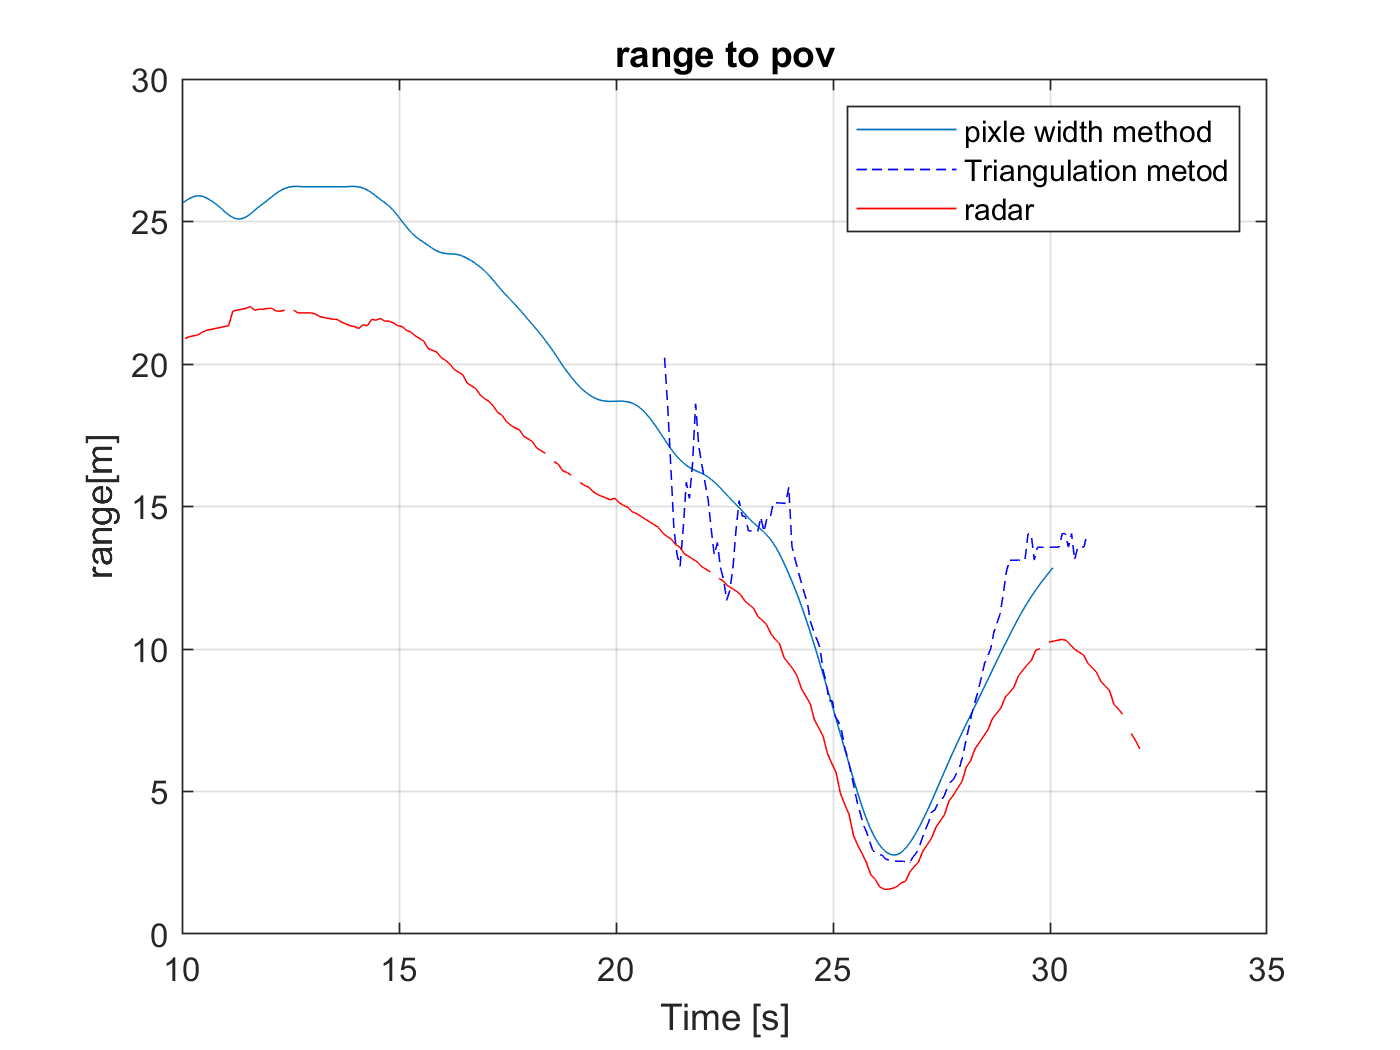
\includegraphics[width=\textwidth]{FiguresMat/homography_compare_long_10794257.png}
    \caption*{Event 1}
\end{minipage}
\begin{minipage}[b]{0.50\textwidth}
    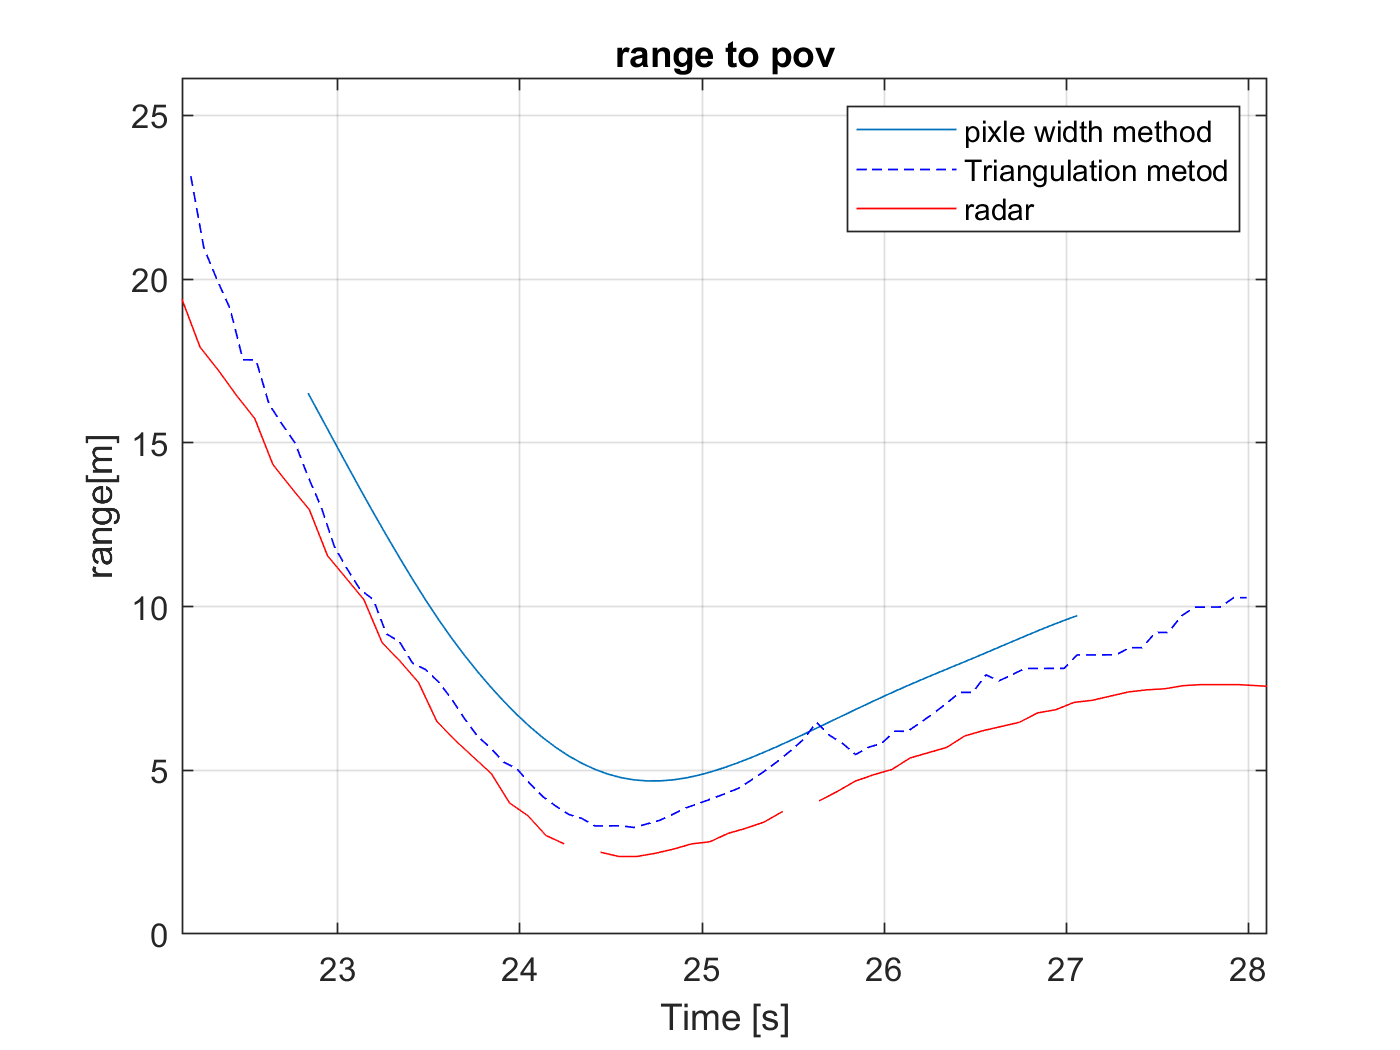
\includegraphics[width=\textwidth]{FiguresMat/homography_compare_long_116147345.png}
    \caption*{Event 2}
\end{minipage}
\caption{Comparing the two methods with Radar Data}
\label{fig:triangulation_comparison_range}
\end{figure}

\subsubsection{Estimation Error}

To understand the performance of the two methods in estimating the range between the SV and POV, some figures were developed that show the relation between the range and its error (Figure \ref{fig:range_error_vs_radar}) as well as the relation between the range and the POV heading angle (Figure \ref{fig:range_error_vs_heading}). 

From Figure \ref{fig:range_error_vs_radar}, three main characteristics are observed. First, and most importantly, both methods show that as the range increases, the error increases. Second, the triangulation method has a lower error on average compared to the pixel width method. Third, the triangulation method has more fluctuation while the pixel width method seems to give more stable ranges. Fourth, at higher ranges there is more fluctuation in the error for both methods.

\begin{figure}[H]
\begin{minipage}[b]{0.49\textwidth}
    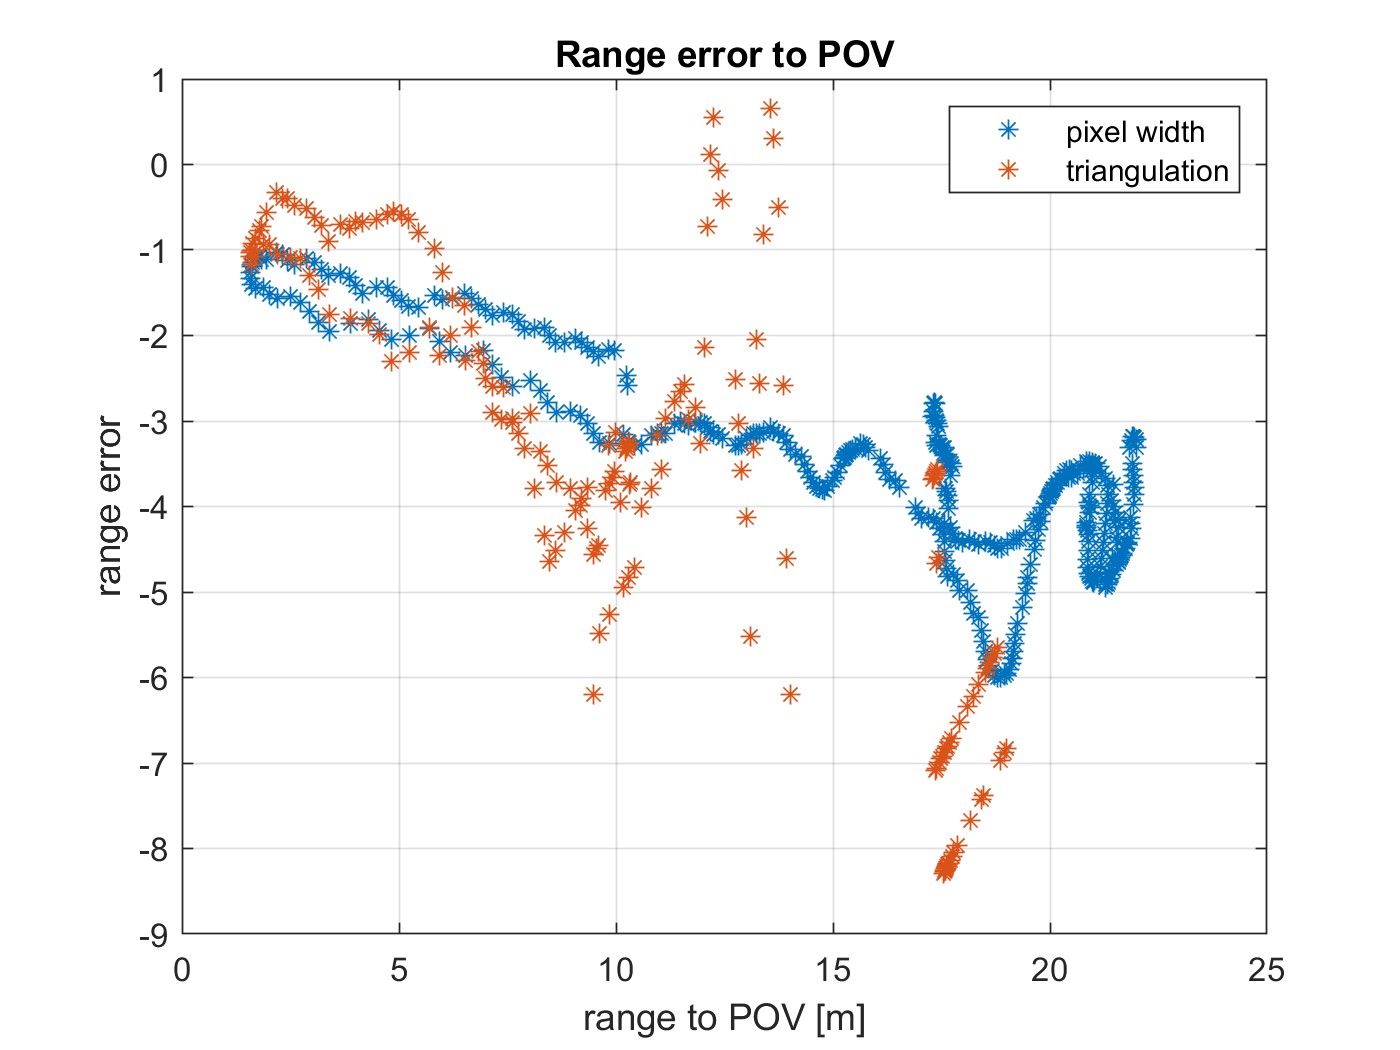
\includegraphics[width=\textwidth]{FiguresMat/range_error_long_10794257.png}
    \caption*{Event 1}
\end{minipage}
\begin{minipage}[b]{0.50\textwidth}
    \includegraphics[width=\textwidth]{FiguresMat/range_error_long_116147345.png}
    \caption*{Event 2}
\end{minipage}
\caption{POV range error vs POV actual range}
\label{fig:range_error_vs_radar}
\end{figure}

From Figure \ref{fig:range_error_vs_heading}, not much can be seen. The results are similar to what was discussed above where the triangulation method is more accurate but less precise compare to the pixel width method. Interestingly, it can be seen from Event 2 of Figure \ref{fig:range_error_vs_heading} that as the heading angle increases, the range error decreases. This is more apparent in the pixel width method.

\begin{figure}[H]
\begin{minipage}[b]{0.49\textwidth}
    \includegraphics[width=\textwidth]{FiguresMat/range_heading_error_long_10794257.png}
    \caption*{Event 1}
\end{minipage}
\begin{minipage}[b]{0.50\textwidth}
    \includegraphics[width=\textwidth]{FiguresMat/range_heading_error_long_116147345.png}
    \caption*{Event 2}
\end{minipage}
\caption{POV range error vs POV estimated heading}
\label{fig:range_error_vs_heading}
\end{figure}

\subsection{Vehicle tracking}
The three methods of tracking that were previously mentioned were studied during the course of project. Due to the time frame of the project, more focus was put on manual annotation, since it was the easiest to implement and was needed for testing other functions in the tool, such as range estimation. Automatic tracking was studied briefly, but was not implemented in the final tool. The results from all there methods are presented below. 

\subsubsection{Manual Tracking}

It was found that this method, although simple, did help identify the POV accurately given the relative speed between the POV and the SV was constant and both vehicles are heading in the same direction, as shown in Figure \ref{fig:POV_tracking_interpolation}, where the user inputs the POV placement in frames 1 and 30, and the tool interpolated the placement in the frames between. In this case, the user was able to track the vehicle in 30 frames through manually defining the POV in only 2 frames. 

\begin{figure}[H]
\centering
\captionsetup{justification=centering}
\begin{minipage}[b]{0.45\linewidth}
    \includegraphics[width=\linewidth]{Figures/interpolation_frame_0.jpg}
    \caption*{User input\\ frame 1 (Green)}
\end{minipage}
\begin{minipage}[b]{0.45\linewidth}
    \includegraphics[width=\linewidth]{Figures/interpolation_frame_10.jpg}
    \caption*{Interpolated POV placement\\ frame 10 (Aqua)}
\end{minipage}
\vspace{5mm}\\
\begin{minipage}[b]{0.45\linewidth}
    \includegraphics[width=\linewidth]{Figures/interpolation_frame_20.jpg}
    \caption*{Interpolated POV placement\\ frame 20 (Aqua)}
\end{minipage}
\begin{minipage}[b]{0.45\linewidth}
    \includegraphics[width=\linewidth]{Figures/interpolation_frame_30.jpg}
    \caption*{User input\\ frame 30 (Green)}
\end{minipage}
\caption{Results from the interpolation method for vehicle tracking}
\label{fig:POV_tracking_interpolation}
\end{figure}

This method becomes less accurate in transient maneuvers, where the relative speed between the vehicles is not constant, i.e the vehicles are braking or accelerating. What this means is that the user would need to annotate more frames for the POV tracking to be more accurate. 

\subsubsection{Automatic and Semi-automatic Vehicle Tracking}
\label{sec:3.6.2}
Automatic vehicle detection was achieved on single images using openCV and a pre-trained neural network called You Only Look Once (YOLO) which is an advanced tool developed for object detection\cite{Redmon_2016_CVPR}, as seen in Figure \ref{fig:yolo_image}.

\begin{figure}[H]
    \centering
    \includegraphics[width=\textwidth]{Figures/yolo_image.jpg}
    \caption{Vehicle detection with the YOLO algorithm}
    \label{fig:yolo_image}
\end{figure}

As seen in the Figure \ref{fig:yolo_image}, YOLO is able to detect the entire vehicle. This is a problem since the method used for range estimation in this project requires only the placement of the rear of the vehicle in the image. This meant that the bounding box marked by YOLO is not on its own usable for range estimation. Instead it would have to be combined with some user defined box around the rear of the vehicle, which would make the tracking semi-automatic. Due to the limited time of this project, this method was not tested.


\subsection{Tool and Graphical User Interface design}

The design of the GUI was kept simple as initially intended, following the same outline described in the methodology section. More focus was put on verifying that the user inputs were processed and used correctly within the program to extract relevant variables. 

\subsubsection{Video player and Controls}

Upon initialization, the user is asked to choose the path of the video that is to be annotated. The user shall then have the option to either re-annotate the data using previously annotated data for the same video, or start over. The video will then be loaded and the user presented with the view shown in  Figure \ref{fig:GUI_overview}.

\begin{figure}[H]
\begin{tikzpicture}
    \node[anchor=south west,inner sep=0] at (0,0) {\includegraphics[width=\textwidth]{Figures/GUI_windoe.jpg}};
    \draw[red,ultra thick,rounded corners] (16,0) rectangle (12.9,12.8) node[above right] {Control button window};
    \draw[green,ultra thick,rounded corners] (12.8,3.4) rectangle  (-0.1,12.8) node[above right] {Main window for video player};
    \draw[blue,ultra thick,rounded corners] (12.8,3.3) rectangle  (-0.1, -0.1) node[below right] {Information window};
\end{tikzpicture}
\caption{Overview of GUI}
\label{fig:GUI_overview}
\end{figure}

\subsubsection{Displaying Information}

% To allow the user to identify how inputs were interpreted by the program, different colors were used to display this information in the main window. Below is a description of how this was achieved. 

% Moreover, a the information window provides information on the current status of the program and what the user should do next.



When a user chooses to input the  placement of different objects in the image, the information window will show what the user has chosen to specify. When the user is defining an object, the figures drawn in the main window are blue, stating the the user is still editing this specific input. When the user presses enter, the input is confirmed and drawn with a different color. These stages are shown in Figure \ref{fig:stages_of_inputs} below. 


\begin{figure}[H]
\centering
\begin{minipage}[b]{0.45\linewidth}
    \includegraphics[width=\textwidth]{Figures/define_vehicle_1.jpg}
    \caption*{User pressed define POV button}
\end{minipage}
\begin{minipage}[b]{0.45\linewidth}
    \includegraphics[width=\textwidth]{Figures/define_vehicle_2.jpg}
    \caption*{User is defining POV (Blue)}
\end{minipage}
\vspace{5mm}\\
\begin{minipage}[b]{0.45\linewidth}
    \includegraphics[width=\textwidth]{Figures/define_vehicle_3.jpg}
    \caption*{User has confirmed the input (Green)}
\end{minipage}
\caption{The different stages of taking user inputs}
\label{fig:stages_of_inputs}
\end{figure}

The same was done for all four input types using blue when the user is editing an input and a different colour when the user has confirmed the input, as seen in 
Figure \ref{fig:define_all}. Moreover, the colour of an interpolated placement is shown in a different colour to help the user know what is user defined and what is interpolated, as seen in Figure \ref{fig:POV_tracking_interpolation}. 

\begin{figure}[H]
    \centering
    \includegraphics[width=\textwidth]{Figures/define_all.jpg}
    \caption{Different colours used for Left lane, Right lane and POV wheels}
    \label{fig:define_all}
\end{figure}

Also, two plots are made in real time as the user is inputting data, as seen in Figure \ref{fig:online_plots}. The first plot shows the calculated range and range rate to the POV. This plot will also plot radar data if that is available. The second plot uses the distances gained from the triangulation method to draw the area around the SV as seen from above. This was especially helpful during the development stage, where these plots helped visualise the output parameters from the tool, such as range, lateral offset and heading angle. 

\begin{figure}[H]
\centering
\begin{minipage}[b]{0.45\linewidth}
    \includegraphics[width=\textwidth]{Figures/GUI_all_inputs.jpg}
    \vspace{2mm}
    \caption*{View in the main window}
\end{minipage}
\begin{minipage}[b]{0.45\linewidth}
    \includegraphics[width=\textwidth]{Figures/online_plot.jpg}
    \caption*{Real-time plot of range and range rate to POV}
\end{minipage}
\begin{minipage}[b]{0.45\linewidth}
    \includegraphics[width=\textwidth]{Figures/GUI_all_inputs_2d.jpg}
    \caption*{Top view plot}
\end{minipage}
\caption{Overview of the different plots}
\label{fig:online_plots}
\end{figure}


\subsubsection{Loading and Saving User Inputs}

Upon selecting a video to annotate, the program will find the event ID from the video name and search in a specified folder for the $.mat$ file containing the time-series data for the SV provided in the SHRP2 data. If no file is found, a message will be printed stating this, but the user will be able to annotate the video nonetheless.

As mentioned in section \ref{sec:Loading_and_saving_data}, two output files are created upon finishing the annotation, one $.mat$ file and on $.pickle$ file, both containing the same data. The $.pickle$ file allows for easier re-annotation of a previously annotated video. Upon selecting a video, the program will search for a $.pickle$ file with the same event ID. If one is found, the user will have the option to either reuse the old annotation and modify it, or start an new annotation.  

\subsubsection{Testing User Sensitivity}

To test the sensitivity of the tool for different annotations, one video was annotated 5 times by the same user, as seen in Figure \ref{fig:same_vid_5times}. The average for all 5 annotations has been computed and compared to the radar range, as seen in Figure \ref{fig:average_vs_radar}.

Initially, this was supposed to be done by all four members of the team. however, due to time constraints, only one member had the time to conduct this test. This was done for Event 1.

\begin{figure}[H]
    \centering
    \includegraphics[width=\textwidth]{Figures/user_comparison.jpg}
    \caption{Same video annotated 5 times by same user}
    \label{fig:same_vid_5times}
\end{figure}

As seen in Figure \ref{fig:same_vid_5times}, at a range of above $\approx 15[m]$, the range is sensitive to user inputs. However, when the range is below  $\approx 15[m]$, the estimated range converges towards the same value for all 5 annotations.

Comparing the average to the radar data, as shown in Figure \ref{fig:average_vs_radar}, provided more accurate results compared to only annotating one time, as in Figure \ref{fig:range_vs_radar_event1}.

\begin{figure}[H]
    \centering
    \includegraphics[width=\textwidth]{Figures/user_average_comparison.jpg}
    \caption{5 time average vs Radar data Event 1}
    \label{fig:average_vs_radar}
\end{figure}




% % Challenges & Limitations
% \section{Challenges and Limitations}
% \label{sec:ChallengesLimitations}
% write here

% Discussion
\section{Discussion}
\label{sec:Discussion}

% The annotation of naturalistic driving data is essential in deriving reliable driver models. It was imperative to idealise a new tool which could make the annotation simpler and faster by making it semi-automatic/automatic. Although the tool is sensitive in some cases, it can be improved with better validation data to benchmark. 

The results presented above are peculiar and interesting. While some deserve to be explained further to understand how they are helpful for the tool development, others should be questioned and criticised. This will be done below in this section.

\subsection{Image Rectification}
While image rectification is a key factor in analysing images to calculate distances, there is not much to say about the results of the image rectifications in this report when it comes to intrinsic parameters. In fact, the values used for intrinsic rectification are provided by VTTI, and although not all cameras in the NDS are the same, the intrinsic rectification provided reasonable results overall.

For the extrinsic parameters on the other hand, the project follows a rather unorthodox approach where not the whole image is rectified for the extrinsic parameters, but only the points needed for calculation. Those points are rectified for the camera's pitch and yaw only, excluding the roll motion of the vehicle since the SV is assumed to be driving in its lane and not making any maneuvers. This rectification was more important for getting a more accurate result for distance calculation, but does not have a drastic effect on the results.

\subsection{Lane Tracking}
Lane detection was observed on variety of spectrum, starting from quality of videos to different types of lanes. The lane detection pipeline included obtaining rectified images, followed by masking, filtering, edge detection and classification of geometry(Hough transform). The results obtained on all quality of videos infer the simplicity and effectiveness of the algorithm, although the lane detection is semi-automatic in nature. It can be further developed as an automatic detection using machine learning optimisation. This further development can benchmark the existing tool. Bird's eye transformation can be explored further by integrating it in the GUI and compare the existing lane detection to draw conclusions on the findings. It is important to notice some of the errors in lane detection like flickering and false detection at times due to wrong masking. This issue can be addressed in the further development. All in all lane detection works well for the naturalistic database used here and functions as a useful technique.


\subsection{Heading Angle}
\label{sec:heading_angle_discussion}
The heading angle, as mentioned earlier, is an important parameter because it helps in the estimation of other parameters such as the longitudinal range between the two vehicles. The method proposed in this project seems to be an innovative method which gives reasonable results. This method however suffers from low precision since it relies on the human annotator to select the right pixels where the wheels of the POV contact the road. Also, in some cases, the wheels are hard to capture, for example when the POV is in front of the SV, or sometimes do not appear on the image.

There was no apparent way to verify the heading angle estimation using the time series data. Instead, the estimated heading angle acquired from the annotation tool was evaluated through first annotating a number videos and then comparing the heading angle visually through studying the footage. According to the visual inspection, the heading angle estimation seemed to be accurate, reaching $0[rad]$ when the POV is moving parallel to the lane and reaching a reasonable maximum value when the POV is cutting in-front of the SV, as shown in Figure \ref{fig:heading_angle}.

To understand the effect of the heading angle on the estimation of the other parameters, the error of those parameters were measured as a function of heading angle. The results were shown in Figures \ref{fig:lat_offset_error_heading} and \ref{fig:range_error_vs_heading}, and will be discussed below as well.

\subsection{Lateral Offset}
\subsubsection{Filtering}
Applying a filter on the results improved the quality of estimating the speeds, especially at higher distances where the filtering removed irrational sudden jumps in the velocities which are caused by discrete pixel numbers. The results are satisfactory and allow for comparison between the resultant values and radar data. 

The filtering was only applied and tested on the pixel width method, which was used to calculate the velocities. The triangulation method, on the other hand, was only developed for distance calculation. The filtering, which proved to be effective, can be implemented on the triangulation method in order to calculate the POV speed. This would be interesting since the triangulation method showed many fluctuations due to its reliance on human annotations. 

Since the filtering of the data is basic, the team discussed introducing more sophisticated filters to the tool such as frequency filters in further developments.

\subsubsection{Lateral Offset versus Radar Data}

The lateral offset matches the radar data with a reasonably small error. The results from both methods are precise where multiple annotations gave similar results. The pixel width method shows a consistent performance with a persistent offset while the triangulation method has more fluctuations in the results but is reaching more accurate values. The sensitivity of the tool can be enhanced by combining the two methods in a sensor fusion manner in order to reduce the uncertainty of the results and have a more robust estimation.

The error of lateral offset proved to be unaffected by the actual lateral offset when using the pixel width method while no conclusive result was achieved for the triangulation method since there is an error in the plotting of the curves as mentioned earlier (Figure \ref{fig:lat_offset_error_distance}). As for the relation to the heading angle of the POV, Figure \ref{fig:lat_offset_error_heading} showed no certain results and hence it was agreed that further testing of the tool is required in order to reach a rational conclusion.


\subsection{Range Estimation}
\subsubsection{Filtering}
There is not much to add about the filtering of data to what was discussed in the lateral offset method. It is worth mentioning that the filtering has a minor effect on the distance estimations, but the main influence is on the POV estimated velocity.

\subsubsection{Range versus Radar Data}
The estimated distances follow the curves of the radar data to a great extent, especially under 15 [m]. However, it is noticed that the pixel width method has an obvious and constant offset from the radar data as it was seen in Figures \ref{fig:range_vs_radar_event1} and \ref{fig:range_vs_radar_event2}, and it is assumed that this is a calibration issue since, as mentioned earlier, the width of the POV is assumed as well as the relative position between the camera and the radar. Those factors could be the reason for the constant offset when using the pixel width method. Regardless of the aforementioned offset, since the estimation curve follows the same shape of the radar data curve, the resultant range rate is capturing the correct relative speed of the POV with respect to the SV, as seen in Figures \ref{fig:range_vs_radar_event1} and \ref{fig:range_vs_radar_event2}. The triangulation method, on the other hand, seems to record the range more accurately although it suffers from some instabilities, especially if the SV is making harsh manoeuvres.

As for the sensitivity of the estimations in relation to the actual distance, it was revealed that at higher distances, both calculation methods have relatively higher errors up to 8 [m] at a range over 20 [m]. Another interesting observation confirms what has been discussed about the triangulation method over and over: this method shows more fluctuations but has a lower average error. This was proven in Figure \ref{fig:range_error_vs_radar}. When comparing the range errors to the heading angle of the POV, an interesting aspect was noticed, where the range error was decreasing with an increase in the POV heading angle (Figure \ref{fig:range_error_vs_heading}). The result could not be explained by relying on only the two showcased events. In the future, more annotations will be carried out by several annotators, and the results should explain or reject this ambiguity.

\subsection{Vehicle Tracking}
Even though automatic tracking was not achieved, the tool was able to simplify the manual tracking process through interpolating manual inputs. This proved to be capable of tracking the POV with relatively good accuracy for being such a simple method. The downside with this method is that it relies on the annotator marking the rear of the POV correctly. It was found that there are some simple improvements that can be done to the GUI that will help the annotator increase accuracy, as mentioned in following section. 

Automatic tracking was promising and the YOLO is capable of identifying all vehicles in the frame, as shown in Figure \ref{fig:yolo_image}. However, there must still be user input to identify which of the identified vehicles is the POV. It can be assumed that the POV is the closest vehicle, but that was not the case in all events. 

Moreover, as mentioned in section \ref{sec:3.6.2}, the methods used for calculating the range to the POV rely on the rear of the POV begin identified in the frame. The box found by the YOLO in Figure \ref{fig:yolo_image} bounded all the pixels in the frame that contain part of a vehicle.

It was thought that the tracking could be made semi-automatic, where the annotator marked a box around the rear of the POV, and the program would use that and track the vehicle found by the YOLO algorithm across frames. Due to time constrains, however, this method was not tested. 

The next step would be to combine the automatic detection using YOLO with the interpolated user annotation to possibly gain more accurate and faster vehicle tracking.

\subsection{Graphical User Interface}

The user interface and overall programming of the tool functioned well and was responsive to user inputs. The program was made modular with different small functions, which allowed for easier troubleshooting and improving functionality without affecting previous progress.

Computational optimisation was not done which was initially not an issue, since the carried calculations were not CPU intensive. However, real time plotting shown in Figure \ref{fig:online_plots} was slow and caused the program to slow down. This mean that while playing the video with the plotting on, the video would appear to play at about half speed. This was not a big issue for annotation, since all inputs when edited when the video was paused on one frame.  

The change due to user variation shown in Figure \ref{fig:same_vid_5times} was expected. The fact that the results converged at $\approx 15[m]$ was better than initially thought. However, some changes were found that could reduce the variation at distances larger than $\approx 15[m]$. 

One solution would be to enlarge the frame to twice the size. This would effectively have made the POV to look twice as big on the screen, which would have made drawing a box around the rear of the POV easier. This would also have made marking other objects in the frame, such as POV wheels and lanes, easier and more accurate, which would have improved the stability of heading calculation, as discussed in \ref{sec:heading_angle_discussion}. This method was tested briefly, but the resulting distance calculations were wrong, since the pixel size of the POV was doubled. Due to time constraints, the team did not have the time to troubleshoot and fix the distance errors and this method is to be pursued in future work. 
Another solution to improve accuracy was to change the size of the blue box shown in Figure \ref{fig:stages_of_inputs} used to define the rear of the POV. It was found that the thickness of line used to draw this box is 2 pixels wide, which, when the POV is further away than $\approx 15[m]$ was part of what caused the fluctuation seen in Figure \ref{fig:same_vid_5times}. This box was drawn using the $cv2.selectROI()$ function, which does not allow for changing the width of the bounding box. Another, similar function has been developed by the team where all parameters of the box are changeable. However, this was not implemented in the tool due to time constraints, but is relatively easy to add in future work.



% Conclusion
\section{Conclusion}
\label{sec:Conclusion}
To conclude with, this report portrays the development of a tool which can be used for annotating NDD. This tool is designed to estimate several important parameters to help in establishing driver models, specifically tailored to critical lane changes of a POV. Those parameters are the heading angle of the POV, the longitudinal range and the lateral offset between the SV and the POV. The main methods used for estimation are the pixel width method and the triangulation method, each having its own strengths and weaknesses. The tool is also able to detect lanes which would ease the process on the annotator. 

All of this was designed into a convenient GUI designed using python language. In that GUI, the annotator has to manually select, per frame, 2 lane lines, the POV's rear as well as the contact points of the POV's wheels with the ground. The annotation is done on several frames manually and the tool will automatically interpolate the annotations between those frames to make the task easier.

The results of the tool are satisfying. Comparison of some annotated events with radar time-series data showed that the extracted variables are close to the actual radar values. The results revealed the performance of the two discussed methods, where the pixel method showed to be more precise while the triangulation method has a better accuracy.

To further improve the quality of annotation using the tool, simple GUI fixes can be implemented such as resizing image frames by making them bigger and hence easier for manual annotation. Also, better calibration for the estimated variables can be achieved through field testing, as done in \cite{bargman2013using}. As of now, the next step is to use put this tool to use by studying different critical lane change events and recreating the trajectory of the incidents so help analyse such cases. 

% \subsection{Challenges and Limitations}

% \subsection{Future Work}

% % Future Work
% \section{Future Work}
% \label{sec:FutureWork}
% write here

% \vspace{6cm}
% \color{black}
% \noindent\rule[0.25\baselineskip]{\textwidth}{1pt}
% Bibliography
% \small
%\bibliographystyle{unsrt}


\newpage
\bibliographystyle{unsrt}
\bibliography{references}

% \begin{thebibliography}{10}

\newpage
\section{Appendix}
\label{sec:Appendix}
\begin{table}[H]
    \centering
    \begin{tabular}{l|l|l}
         \bf{Notation} & \bf{Name} & \bf{Unit}  \\ \hline
         $a$ & pixel size to left edge of POV & [pixels]\\
         $b$ & pixel size to right edge of POV & [pixels] \\
         $C$ & camera's center & \\
         $D$ & longitudinal distance & [m] \\
         $D_x$ & lateral distance & [m] \\
         $D_y$ & longitudinal distance & [m] \\
         $f_u$ & focal length in u-direction & [pixels] \\
         $f_v$ & focal length in v-direction & [pixels]\\
         $HA$ & heading angle of POV & [rad] \\
         $H$ & height of camera from ground & [m] \\
         $\bf{H}$ & homography matrix & \\
         $k_1$ & radial distortion coefficient 1 & \\
         $k_2$ & radial distortion coefficient 2 & \\
         $k_3$ & radial distortion coefficient 3 & \\
         $l$ & arbitrary scaling factor & \\
         $L$ & lateral distance from camera center & $[m]$\\
         $m$ & slope of line & \\
         $P$ & point in 3D &  \\
         $p$ & point in image frame post rectification & \\
         $p'$ & point in image frame pre rectification & \\
         $p_1$ & tangential distortion coefficient 1 & \\
         $p_2$ & tangential distortion coefficient 2 & \\
         $\psi$ & camera yaw angle & [rad]\\
         $\phi$ & camera roll angle & [rad]\\
         $\bf{R}$ & Euler-Rodrigues rotation matrix & \\
         $\theta$ & camera pitch & [rad]\\
         $u$ & u in uv image coordinate frame & [pixels] \\
         $v$ & v in uv image coordinate frame & [pixels] \\
         $w$ & width of POV in image & [pixels] \\
         $w'$ & corrected width of POV in image & [pixels] \\
         $W$ & width of POV in real life & \\
         $x$ & x in xy image coordinate system & [pixels] \\
         $x'$ & x coordinate pre-rectification & [pixels] \\
         $X$ & X in 3D coordinate frame & [m] \\
         $y$ & y in xy image coordinate system & [pixels] \\
         $y'$ & y coordinate pre-rectification & [pixels] \\
         $Y$ & Y in 3D coordinate frame & [m] \\
         $Z$ & Z in 3D coordinate frame & [m] \\
    \end{tabular}
    \caption{Table of notations}
    \label{tab:notations}
\end{table}


\begin{table}[H]
    \centering
    \begin{tabular}{c|c}
        package & version\\
        \hline
        Python & 3.7.1  \\
        openCV & 4.1.1 \\
        numpy & 1.16.4\\
        scipy & 1.2.1\\
        tkinter & 8.6.8\\
        matplotlib & 3.1.0\\
    \end{tabular}
    \caption{Python modules and libraries}
    \label{tab:python_modules}
\end{table}


% \end{thebibliography}





\end{document}